\documentclass[12pt]{report}
\usepackage{setspace, psfrag}
\usepackage{graphicx}
\usepackage{amssymb, amsmath}
\usepackage{emptypage}

\graphicspath{ {figures/} }

\usepackage[nottoc]{tocbibind}

\usepackage[utf8]{inputenc}
\usepackage[backend=biber]{biblatex}
\addbibresource{ucscamsms2015.bib}
\usepackage{url}
\setcounter{biburllcpenalty}{7000}
\setcounter{biburlucpenalty}{8000}

\usepackage{hyperref}
\hypersetup{
  colorlinks=true,
  linkcolor=black,
  citecolor=red,
  urlcolor=blue,
  breaklinks=true
}


% Taken from pandoc x.md -o test.tex --standalone
% Coloring below is based on the One Light syntax theme in Atom text editor
\usepackage{color}
\usepackage{fancyvrb}
\newcommand{\VerbBar}{|}
\newcommand{\VERB}{\Verb[commandchars=\\\{\}]}
\DefineVerbatimEnvironment{Highlighting}{Verbatim}{commandchars=\\\{\}}
\newenvironment{Shaded}{}{}
\newcommand{\KeywordTok} [1]{\textcolor[RGB]{77,107,200}{{#1}}}
\newcommand{\DataTypeTok}[1]{\textcolor[RGB]{77,107,200}{{#1}}}
\newcommand{\DecValTok}  [1]{\textcolor[RGB]{157,61,0}{{#1}}}
\newcommand{\BaseNTok}   [1]{\textcolor[RGB]{0.25,0.63,0.44}{{#1}}}
\newcommand{\FloatTok}   [1]{\textcolor[RGB]{157,61,0}{{#1}}}
\newcommand{\CharTok}    [1]{\textcolor[RGB]{96,172,57}{{#1}}}
\newcommand{\StringTok}  [1]{\textcolor[RGB]{96,172,57}{{#1}}}
\newcommand{\CommentTok} [1]{\textcolor[RGB]{166,162,140}{{#1}}}
\newcommand{\OtherTok}   [1]{\textcolor[RGB]{215,55,55}{{#1}}}
\newcommand{\AlertTok}   [1]{\textcolor[RGB]{1.00,0.00,0.00}{{#1}}}
\newcommand{\FunctionTok}[1]{\textcolor[RGB]{0.02,0.16,0.49}{{#1}}}
\newcommand{\ErrorTok}   [1]{\textcolor[RGB]{1.00,0.00,0.00}{{#1}}}
\newcommand{\NormalTok}  [1]{{#1}}


\setlength{\textwidth}{6.15in}
\setlength{\textheight}{8.5in}
\addtolength{\oddsidemargin}{-0.25in}
\addtolength{\topmargin}{-0.5in}
\doublespacing
\raggedbottom

\usepackage[intoc]{nomencl}
\makenomenclature

\begin{document}

\begin{titlepage}
\begin{center}

\textsc{\Large University of California \\
Santa Cruz } \\
\vspace*{0.15in}

\textsc{\Large \textbf{Optimal schedules for tasks \\
with stochastic runtimes}}
\vspace*{0.15in}

\large
A project submitted in partial satisfaction \vspace*{-0.1in} \\
of the requirements for the degree of \\
\vspace*{0.15in}

\textsc{\Large Master of Science} \\
\large in \\

\textsc{\Large Statistics and Applied Mathematics} \\
\large by \\
\vspace*{0.15in}

\textbf{Niranjan Vissa} \\
\vspace*{0.15in}

August 2015
\large
\vspace*{0.15in}

\begin{flushright}

The Project of Niranjan Vissa \\
is approved:
\vspace*{-0.1in}
\vspace*{0.2in}

\rule{2.5in}{.01cm}

Professor David Draper

\vspace*{0.2in}

\rule{2.5in}{.01cm}

Professor Herbert Lee

\end{flushright}

\end{center}
\end{titlepage}


\pagenumbering{roman}

\setcounter{page}{2}

\newpage

\mbox{}

\newpage
\begin{center} \textbf{\large ACKNOWLEDGEMENTS} \end{center}
\bigskip
\noindent
To be completed

\newpage

\singlespacing

\tableofcontents

\setcounter{tocdepth}{2}

\listoftables

\listoffigures

\newpage
\renewcommand{\nomname}{Notation}
\printnomenclature

\newpage
\pagenumbering{arabic}

\chapter{Introduction}

\section{Background on Cloud Computing}

A recent trend in the IT industry has been the emergence of \textit{cloud computing}, in which computing infrastructure is maintained in one or more large data centers and offered for use via a network connection \cite{Interoute:WhatIsCloudComputing}.
The main advantages of such a setup are sharing of resources, economies of scale and flexibility to use as much or as little of the computing infrastructure as needed.
This is in contrast to traditional computing infrastructure setups, where there is little flexibility and clients have to predict future computing needs well in advance.
The predictions determine the infrastructure to purchase and are often incorrect, resulting in under-investment or over-investment in infrastructure.
Other advantages of a cloud computing setup include instant access to a vast and varied amount of computing resources, flexible pricing where the client only pays for the resources used and avoidance of a single point of failure due to the way clients access the computing infrastructure and the redundancies built in to this infrastructure.

Cloud computing offerings can be classified into three broad types.
The first type is Infrastructure-as-a-Service (IaaS), where only basic virtualized environments running on physical hardware are available.
Everything from the operating system upwards must be installed and maintained by the client.
This is useful when the client wants complete control over the software environment but does not want to deal with maintaining hardware or virtualized environments.
The second type of offering is Platform-as-a-service (PaaS), where the cloud service provider offers a virtualized environment with an operating system and common software required by most applications.
The provider takes care of maintaining and updating this software, while the client focuses on building custom applications.
The last type is Software-as-a-Service (SaaS), where entire software applications are offered on demand.
In this setup, software applications are \textit{rented} from the provider and are accessed over a network connection instead of being purchased and installed on the client's computing infrastructure.
In all the above cases, the hardware is usually shared across multiple clients and access to hardware is abstracted away from the client.

Cloud computing offerings can also be classified as \textit{private clouds} or \textit{public clouds}.
Private clouds are virtualized environments that are meant for the use of a single client and are accessed via a secure, private network connection.
They cannot be accessed by anyone else.
A public cloud, in contrast, is owned and operated by a cloud service provider and can be utilized by anyone who wants to rent infrastructure or software on demand.
It is accessed via a public network like the internet.
Examples of public clouds include Amazon Web Services from Amazon.com, Inc., Azure from Microsoft, Inc. and Google Cloud Platform from Google, Inc.
This report deals only with PaaS offerings from public clouds, though the findings are equally applicable to private clouds.

The availability of a large amount of computing resources on demand and the ability to pay for these resources by the hour have enabled the migration of many workloads to a cloud computing environment \cite{RightScale:2015}.
These workloads can be processed in parallel on multiple resources and can complete much quicker than if they were processed on a single resource.
While there is no practical constraint on the number of resources that can be used, budgetary constraints usually limit the number and type of resources that can be used to process a workload.
Thus, there is always a trade-off between the benefit arising from processing a workload quickly and the cost of resources used to process the workload.

In most cases, the benefit is a fixed value and is paid out when all tasks in the workload are completed by a given deadline.
It does not increase if the tasks are completed earlier and will not be paid out if tasks are not completed by the deadline.
The only way for the client to maximize the benefit is to complete all tasks by the deadline with the lowest possible processing costs.
The rest of this report deals with developing efficient methods of scheduling tasks in parallel on multiple resources to achieve this goal.


\section{Background on Scheduling}

\label{SchedulingOverview}
Scheduling refers to the process of assigning tasks to resources that complete the tasks.
It is a common problem and arises in a variety of everyday situations, such as scheduling manufacturing tasks in factories, takeoffs and landings of planes in airports, sports tournaments, nurse shifts in hospitals and 	tasks across multiple computers. \cite{Hoos2004}.

The input to a scheduling problem is a set of tasks to be completed and a set of resources that can process the tasks.
The output is a schedule that maps tasks to resources in a certain order.
Scheduling problems are typically subject to various feasibility constraints that define a valid schedule.
Examples of such constraints include maintaining minimum time intervals between plane takeoffs and landings, avoiding adjacent shifts for nurses, completing tasks by a certain deadline and using a fixed number of machines.
Once a set of feasible schedules is available, various optimization criteria are used select the best schedule from this set.
Examples of such criteria include minimizing total weighted delay over all flights, preference of nurses for certain shifts and minimizing maximum completion time for tasks.

Scheduling problems can be classified in various ways based on task characteristics, resource characteristics and the type of optimization criteria used \cite{Hoos2004, Pinedo2012}. 
Task characteristics include pre-emption, release times, deadlines, dependencies, weights and amount of pre-processing.

\textit{Pre-emption} refers to the interruption of a task in progress so that it can be re-started later on the same or different resource.
\textit{Pre-emptive} schedules allow tasks to be interrupted while \textit{non-pre-emptive schedules} do not allow pre-emption: once a task has started processing on a certain resource, it must complete processing on the same resource.

Tasks can be associated with release times and deadlines.
Release time for a task represents the earliest time a task is available for processing.
A task cannot start processing before its release time.
A deadline represents the time by which a task must complete processing.
When a set of tasks is associated with a release time, none of the tasks can begin processing before the release time.
Similarly, when a set of tasks is associated with a deadline, all tasks in the set must complete processing by the deadline.

Dependencies between tasks control the order in which tasks can be processed.
Examples of dependencies include precedence constraints between tasks, where one task depends on other tasks and cannot start processing until all tasks on which it depends have completed.
Task weights and the amount of pre-processing tasks have received also influence the types of schedules that can be generated.
Tasks with higher weights must usually be processed first and tasks that have been pre-processed typically require less processing time.

Scheduling problems can also be classified by the properties of resources.
Tasks can be processed on a single resource or by multiple resources in parallel.
When using resources in parallel, the resources can be \textit{identical} or \textit{unrelated}.
Identical resources are all of the same type; task runtime will be the same regardless of which resource is used to process the task.
When using unrelated resources in parallel, runtime for a task depends on the resource used to process the task and might vary for each resource.

Finally, scheduling problems can be classified by the the type of optimization criteria used to select the best schedule from a set of feasible schedules.
Examples of such criteria include minimizing the maximum completion time (also known as \textit{makespan}) of a set of tasks; minimizing the weighted completion time of a set of tasks where each task is assigned a weight proportional to its benefit; and minimizing the maximum delay of a set of tasks, if the tasks are associated with a deadline.

In this work, I focus on the problem of finding optimal non-pre-emptive schedules that minimize makespan while processing a set of tasks on multiple identical resources in parallel. All tasks have the same weight, have not undergone any pre-processing and are immediately available for processing.

\nomenclature{$\mathcal{I}$}{Set of instances available to process tasks. Each instance is associated with a \textit{type} $Y$ and a \textit{cost} $C$.}
\nomenclature{$\mathcal{T}$}{Set of input tasks that must be processed. Each task is associated with a \textit{length} $L$.}

\nomenclature{$B$}{Benefit (specified in dollars) paid out when all tasks in $\mathcal{T}$ are completed by the deadline. If {$\mathcal{T}$} is not complete by the deadline, $B=\$0$.}
\nomenclature{$D$}{Deadline (specified in hours) by which all tasks in $\mathcal{T}$ must complete processing}
\nomenclature{$L_i$}{Length of task $T_i$}
\nomenclature{$R_{ij}$}{Runtime of task $T_i$ on instance $I_j$; known only when $T_i$ completes processing on $I_j$; all instances of the same type are assumed to process the task in the same amount of time}
\nomenclature{$R_j$}{Total runtime of all tasks assigned to instance $I_j$}
\nomenclature{$M_S$}{Makespan of schedule $S$ to process the set of tasks $\mathcal{T}$}
\nomenclature{$C_j$}{Cost per hour of instance $I_j$ (specified in dollars/hour)}
\nomenclature{$S$}{A schedule that maps tasks to resources that can process the tasks}
\nomenclature{$U_{km}$}{Utility of a schedule using $m$ instances of type $k$}

\section{Problem Formulation}

The previous sections highlight the need for efficient scheduling methods to complete a set of tasks on time \underline{and} with the lowest possible processing cost.
This section specifies the problem in detail and suggests a possible solution.
Subsequent sections develop this solution and show that it solves the problem in an efficient manner.

Let $\mathcal{T} := {T_1, T_2, \dots, T_n}$ be the set of input tasks that must be processed.
This set of tasks is associated with a benefit $B$ specified in dollars and a deadline $D$ specified in seconds.
Each task $T_i$ is independent of all other tasks in $\mathcal{T}$, so tasks can be processed in any order.
$\mathcal{T}$ is considered to complete when all tasks in $\mathcal{T}$ are complete.

Let $\mathcal{I} := {I_1, I_2, \dots, I_m}$ be the set of resources (also known as instances in this report) available to process tasks in $\mathcal{T}$.
These instances are grouped into various instance types depending on their configuration.
Let $r_{ij}$ be the runtime of task $T_i$ on instance $I_j$.
Time taken to complete a task depends on the type of instance on which the task is processed; slower instances will take more time to process the same task compared to faster instances.
Let $C_j$ be the cost per hour of instance $I_j$ (specified in dollars), with slower instances costing less than faster instances.

Let $S$ be a schedule and let $t_{I_j}$ be the index of the tasks in $\mathcal{T}$ assigned to instance $I_j$ by $S$.
The total runtime $R_j$ for all jobs assigned to instance $I_j$ is called the  \textit{load} on instance $I_j$ and is defined as

\begin{equation}
\label{eq:def:load}
R_j = \sum_{k \in t_{I_j}} r_{kj}
\end{equation}

The maximum runtime across all instances or the \textit{makespan} $M$ of $S$ is then defined as:

\begin{equation}
\label{eq:def:makespan}
M = \max_{j \in \mathcal{I}} {R_j}
\end{equation}

The makespan of a schedule represents the time taken by the schedule to complete all tasks and determines if the tasks will be completed by the deadline.
A \textit{feasible} schedule is defined as a schedule with $M \le D$.

Makespan depends on the number of tasks, the number of instances and the type of instances used to process tasks.
The number of tasks is an input to the problem, so the only parameters that can be varied are the number and type of instances.
Makespan will be lowest when each task is processed in parallel on a separate instance of the fastest instance type and highest when all tasks are processed sequentially on a single instance of the slowest instance type.
Processing cost depends on the number and type of instances used and the amount of time these instances were used.

To find a feasible schedule with the lowest processing cost, I need to evaluate schedules on a variety of instances types and vary the number of instances used in each case.
The number of instances that a schedule can use can vary from 1 to the number of input tasks.
A schedule can use any instance type whose configuration satisfies the minimum requirements of the tasks.
I simplify our situation by assuming that a schedule can only assign tasks to instances of the same type, i.e., tasks can only be assigned to, say, 5 instances of a certain type, not 3 instances of one type and 2 instances of a different type.
This constraint leads to the identical parallel machines scheduling problem.
It has the advantage of restricting our search space but the disadvantage of excluding schedules that might be more optimal than what I can find when I use a single instance type in a schedule.

Section \ref{SchedulingOverview} mentions that the set of feasible schedules is first enumerated and the optimal schedule is then selected from this set.
To obtain the set of feasible schedules, the makespan for all possible schedules must be calculated and compared to the deadline to determine feasibility.
But the number of possible schedules is typically very large.
The \textit{Bell number} \cite{mathworld:bellnumber} refers to the number of ways a set with $n$ elements can be partitioned into subsets such that each element is present in exactly one subset.
Here each partition of the input set of tasks refers to a possible schedule.
A set of 10 tasks can be assigned to instances into $115,975$ ways, with the number of instances varying from 1 to 10.
20 tasks result in $50 \times 10^{12}$ schedules on 1 to 20 instances and 100 tasks result in $~ 4 \times 10^{115}$ schedules on 1 to 100 instances.
Thus, even with a small number of tasks, the number of possible schedules is too large to exhaustively evaluate for feasibility.
So it is not possible to first enumerate the subset of feasible schedules and then select the schedule with the lowest processing cost.

To work around this, I use \textit{stochastic optimization} methods to find feasible schedules while simultaneously keeping track of their processing cost.
Starting from an initial schedule, I determine if it is feasible.
If it is not, I reject the schedule; if it is, I keep track of its processing cost and this schedule become the candidate solution.
Stochastic local search methods are used to find other feasible schedules in the neighborhood of the current schedule that might have a lower processing cost.
I continue the search in this manner until the termination criterion is met.
When the search terminates, the feasible schedule with the lowest processing cost is the optimal schedule.
A feasible schedule may not be found if the deadlines for the set of tasks are unrealistic.
Even if the deadlines are realistic and a feasible schedule does exist, the benefit associated with a set of tasks may be lower than the lowest possible processing cost for the tasks and it will be more beneficial to not process the tasks than to process the tasks and incur a loss.
To avoid these situations, I assume that the deadlines are always realistic and the benefit is higher than the lowest possible processing cost.

To evaluate feasible schedules, I adopt a \textit{decision-theoretic} framework and \textit{maximize expected utility} \cite{BernadoSmith} to select the best schedule.
One possible \textit{utility} function evaluating a schedule using $m$ instances of type $k$ can be expressed as:

\begin{equation}
\label{eq:def:utility:deterministic}
	U_{km} = B - \left(\sum_{j=1}^{m} R_{j} \right) \cdot C_k
\end{equation}

where $U_{km}$ is the utility of a schedule using $m$ instances, each of type $k$, $B$ is the benefit derived from processing all tasks by the deadline $D$, $C_k$ is the cost per hour of an instance of type $k$ (fixed and known in advance), and $R_j$ is the total time used by instance $I_j$ of type $k$, rounded up to the next hour.
Note that both terms on the right-hand side of equation (\ref{eq:def:utility:deterministic}) are specified in the same units: $B$ in dollars, $C_k$ in dollars per hour and $R_j$ in seconds (which when converted to hours and multiplied by $C_j$ gives dollars).

Since all schedules have the same benefit, (\ref{eq:def:utility:deterministic}) simplifies to:

\begin{equation}
\label{eq:def:utility:deterministic:simplified}
	U_{k,m} = - \left(\sum_{j=1}^{m} R_{j} \right) \cdot C_k
\end{equation}

Expected utility is maximized when the term of the right in Equation \ref{eq:def:utility:deterministic:simplified} (processing cost) is as small as possible.

An implicit assumption in (\ref{eq:def:utility:deterministic:simplified}) is that the task-level runtimes $r_{ij}$ and instance-level runtimes $R_j$ are deterministic and known in advance.
But this is not always the case.
It is not uncommon to find situations where the runtime of a task is known only when the task completes processing.
In such cases, the runtimes are usually distributed according to a probability distribution that is known in advance.
Each runtime can be distributed according to a different probability distribution.
In some cases, even the form of the probability distribution is not known or has no closed form expression.
In these cases, the distribution of task runtimes must be determined empirically as described in the next section.

When runtimes are stochastic, (\ref{eq:def:utility:deterministic:simplified}) becomes:

\begin{equation}
\label{eq:def:utility:stochastic}
	E(U_{km}) = - \bigg[(\sum_{j=1}^{m} \sum_{k \in t_{I_j}} E(r_{kj}) \bigg] \cdot C_k
\end{equation}

where $t_{I_j}$ is the index of the tasks in $\mathcal{T}$ assigned to instance $I_j$ by $\mathcal{S}$, $E(U_{km})$ is the expected utility of a schedule using $m$ instances of type $k$ and I maximize \textit{expected} utility by averaging over all possible runtimes.

Schedules for tasks with stochastic runtimes have stochastic makespans that have their own probability distribution. In this case, I relax our definition of feasibility so that any schedule with a makespan whose 95th percentile is $\le D$ is considered feasible. A major contribution of the current work is a method to find a feasible schedule with the lowest processing cost when tasks have stochastic runtimes that are distributed according to known or unknown probability distributions.

\section{Data}

\label{Data}
The data for this problem is as follows:

\begin{itemize}
\item \textbf{Instance types:}
Each Amazon data center has hundreds of thousands of virtual machines  (also known as instances) \cite{AWS:EC2} running on physical hardware.
Each instance is associated with a certain configuration of instance type and speed, memory, local disk space and network speed.
This configuration of resources represents an instance type.
Examples of instance types include compute-optimized instance types with faster, more powerful instances, memory-optimized instance types with large amounts of memory and storage-optimized instance types with large amounts of local disk space.
There are dozens of such instance types and thousands of instances of the same type in each data center.
The instance types and the number of instances of a certain type represent the action space of the decision problem.
In this work, I assume that tasks are constrained only by processor speed and not by any other resource.

\item \textbf{Task lengths}:
The input to the problem is a set of tasks.
Each task is associated with a property called \textit{length}.
Runtime for a task is roughly proportional to its length.
Besides length, other properties of the task also influence task runtime.
If these properties were easy to quantify, then runtime would be a deterministic function of length and the other properties.
But these properties are not easily quantifiable, so task runtime is considered to be a random unknown with length as the only co-variate that can be used to predict runtime.
Note that task runtime depends on task length and the instance type on which the task is running.

\end{itemize}

\chapter{The single instance case}

This chapter focuses on selecting optimal feasible schedules when processing tasks on a single resource, and the next chapter deals with the case of processing tasks on multiple identical resources in parallel.

\section{Method}

Equation (\ref{eq:def:makespan}) defines the makespan of a schedule as the maximum load across all instances used by the schedule.
When a schedule processes tasks on a single instance, there is only one possible schedule and the makespan of this schedule is the same as the load on the given instance.
This makespan is invariant to the order in which tasks are processed on the instance.
Since the number of instances is fixed at 1, the action space is reduced to the set of instance types that result in feasible schedules, and the action is the selection of the instance type from this set that maximizes (expected) utility.

When task runtimes are deterministic and known in advance, the makespan $M$ of a schedule $S$ using instance type $k$ is just the sum of the runtimes for $k$.
If $M \le $ deadline $D$, then $S$ is feasible and the utility $U_{k1}$ is calculated for these instance types as shown in equation (\ref{eq:def:utility:deterministic:simplified}) with $m=1$.
This process is repeated for each instance type in the action space and the feasible schedule with the maximum utility is the solution to the problem.
All tasks should be processed on the instance type associated with this schedule.

When runtimes are stochastic, $M$, which is the sum of runtimes, is itself random with an associated probability distribution.
The distribution of $M$ depends on the nature and number of runtime distributions being summed.
Tasks in $\mathcal{T}$ are assumed to be independent and represent a random sample from the population of tasks.
The same applies to the runtimes of these tasks.
If the number of tasks or, equivalently, runtimes, is a large enough number, say, 100, then the Central Limit Theorem (CLT) applies and $M$ will have a \textit{Normal} distribution.
The mean and variance of the Normal distribution will equal the sum of the means and variances, respectively, of the individual runtime distributions.
If the number of tasks is not large enough for the CLT to apply, then the distribution of $M$ depends on the nature of the distributions being summed.
If the runtimes all have distributions that are members of the same family, it is possible for $M$ to have a distribution of this family whose parameters are a simple function of the parameters of the individual runtime distributions.
For instance, if the individual runtimes distributions are all Poisson distributions, then $M$ will also have a Poisson distribution whose parameter is the sum of the parameters of the individual Poisson distributions.

If the runtime distributions are not members of the same family or the distribution of $M$ cannot be determined easily from the individual distributions, then the distribution of $M$ can be determined via bootstrap resampling \cite{Efron1993}.
A value is randomly sampled from the runtime distribution of each of the input tasks.
These values are then summed to give a value for makespan.
This process is repeated a large number of times, resulting in a bootstrap distribution for makespan.

In all the above cases, the $95th$ percentile of the makespan distribution is assumed to represent the makespan of the input set of tasks on the instance type under consideration.
This value is used to calculate (expected) utility and determine the instance type that maximizes (expected) utility.


If the runtime distribution for one or more tasks is unknown or does not have a closed form expression, a value must be sampled from the empirical distribution for the runtime.
The empirical runtime distribution for a task with length $l$ on an instance of type $k$ is determined by processing a number of samples of tasks with length $l$ on an instance of type $k$ and recording the runtimes.
This set of runtimes represents the empirical probability distribution for the runtime and can be sampled to get a value for the runtime of the associated task.

\section{Validation}

\label{validate:runtimes:deterministic}
When runtimes are deterministic and known in advance, determining the makespan is straightforward. 
Table \ref{table:validate-1instance-deterministic} shows the details for a set of 5 tasks associated with a benefit of \$30 and a deadline of 25 hours. 
These tasks can run on 3 different instance types A, B, and C. 
The instance types vary in their cost and speed of processing, with the cheaper types being slower than the more expensive types. 
Makespan is rounded up to the next hour since I pay for the entire hour even if I use only a fraction of the hour. 
Only B and C result in feasible schedules (makespan $\leq$ deadline ) with C having the maximum utility even though it has the highest cost per hour.
The schedule using instance type C is the optimal schedule for the given set of tasks.

\begin{table}[h]
\centering
\begin{tabular}{l|l|l|l|l|l}
{\bf \begin{tabular}[c]{@{}l@{}}Instance \\ type\end{tabular}} & {\bf 
	\begin{tabular}[c]{@{}l@{}}Relative \\ Speed\end{tabular}} & {\bf 
	\begin{tabular}[c]{@{}l@{}}Cost \\ (\$/hr)\end{tabular}} & {\bf \begin{tabular}[c]{@{}l@{}}Runtimes \\ (hr)\end{tabular}} & {\bf \begin{tabular}[c]{@{}l@{}}Makespan\\ (hr)\end{tabular}} & {\bf \begin{tabular}[c]{@{}l@{}}Utility \\ (\$)\end{tabular}} \\ 
A                                                            & 1  & 1                                                             & 5.2, 8.5, 2.5, 4.1, 6.0                                        & 27                                                          & ---                                                              \\ \hline
B                                                            & 1.07  & 1.1                                                           & 4.84, 7.91, 2.33, 3.81, 5.58                                   & {\bf 25}                                                   & 3.09                                                          \\ \hline
C                                                            & 1.35  & 1.3                                                           & 3.85, 6.29, 1.85, 3.03, 4.44                                   & {\bf 20}                                                   & {\bf 4.7}                                                     \\ \hline
\end{tabular}
\caption{\textit{Calculating utility for a set of tasks whose runtimes are deterministic and known in advance. The benefit is \$30 and the deadline is 25 hours.}}
\label{table:validate-1instance-deterministic}
\end{table}

\subsection{$\geq 100$ tasks/instance}

When 100 or more input tasks with stochastic runtimes are submitted, the makespan has a Normal distribution by the Central Limit Theorem (CLT).
(100 is an arbitrary threshold chosen to satisfy the 'sufficiently large number of values' assumption of the CLT).
To validate the above method, tasks are chosen whose actual runtimes are known.
These runtimes represent the 'truth' and are used to calculate the true optimal schedule as shown in Section \ref{validate:runtimes:deterministic}. 
This true optimal schedule is then compared to the predicted optimal schedule to determine the effectiveness of the above method. 

Each schedule is associated with an instance type, makespan and processing cost. 
Processing cost is a constant times the makespan, so minimizing makespan on the optimal instance also minimizes the processing cost.
I consider a predicted optimal schedule to be equivalent to the true optimal schedule if the instance types of both schedules are identical and the 95\% confidence interval for predicted makespan contains the true makespan.
This confidence interval is based on a Normal approximation to the makespan distribution.
95\% is again an arbitrary threshold and was chosen since it is considered to be 'close enough' to the optimal makespan by most people.

\begin{figure}
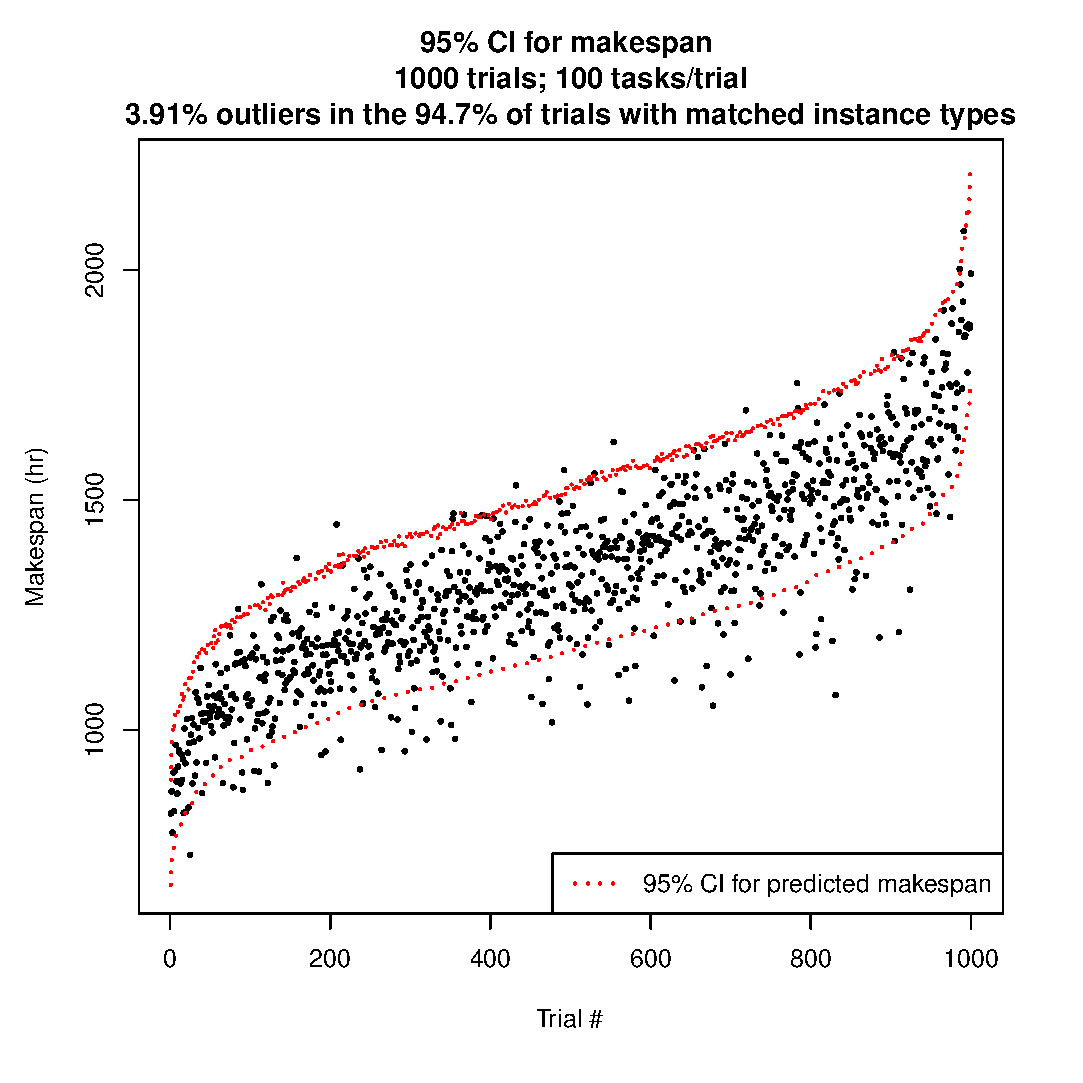
\includegraphics[width=1\textwidth]{validate-stochastic-runtimes-1000-trials-100-tasks.eps}
\caption{\textit{95\% confidence interval for makespan using Normal approximation when 100 tasks are processed on a single instance. Data sorted by lower bound of 95\% CI.}}
\label{fig:validate-stochastic-runtimes-1000-trials-100-tasks}
\end{figure}

I decided to validate collections of tasks containing 100, 250, 500 and 1000 tasks. 
1000 collections of tasks were generated for each of the above sizes (e.g., 1000 sets of 100 tasks each).
For each task in each collection, runtime was sampled from one of four distributions with positive support (Poisson, Exponential, Gamma and Uniform).
The parameters for these distributions were arbitrary and could be different for different tasks.
For each task, the distribution and parameters used were recorded.
So 100 tasks in a collection, for instance, could contain runtimes from all 4 distributions in different quantities.
The true optimal schedule (instance type and makespan) was calculated for each collection of tasks using the sampled values assuming an action space of the 3 simulated instance types (A, B and C) mentioned in the previous section.
Distribution information for each task was used to predict the makespan distribution and the optimal schedule.

Figure \ref{fig:validate-stochastic-runtimes-1000-trials-100-tasks} shows the results of these predictions when processing 100 tasks at a time.
Each black point represents the true makespan for a set of 100 tasks.
There are 1000 such points in the plot.
The red dots represent the 95\% confidence interval for predicted makespan based on a Normal approximation to the makespan distribution.
94.7\% of the predicted schedules used the optimal instance type while the remaining 5.3\% used a sub-optimal instance type.
Of the predictions using the optimal instance type, the 95\% confidence interval for predicted makespan contained the true value in all but 3.91\% of the cases.
So the 95\% CI for predicted optimal schedule effectively contained around 91\% of the true optimal schedules.
Figures \ref{fig:validate-stochastic-runtimes-1000-trials-250-tasks}, \ref{fig:validate-stochastic-runtimes-1000-trials-500-tasks} and \ref{fig:validate-stochastic-runtimes-1000-trials-1000-tasks} show the corresponding results when processing 250, 500 and 1000 tasks/instance respectively on the same 3 instances types. 
In these cases, the method performs better and the confidence intervals contain almost 95\% of the true optimal schedules.
When the runtime distributions are unknown, runtimes are sampled from the corresponding empirical distributions. 
Results in this case are very similar and are not shown.

\begin{figure}
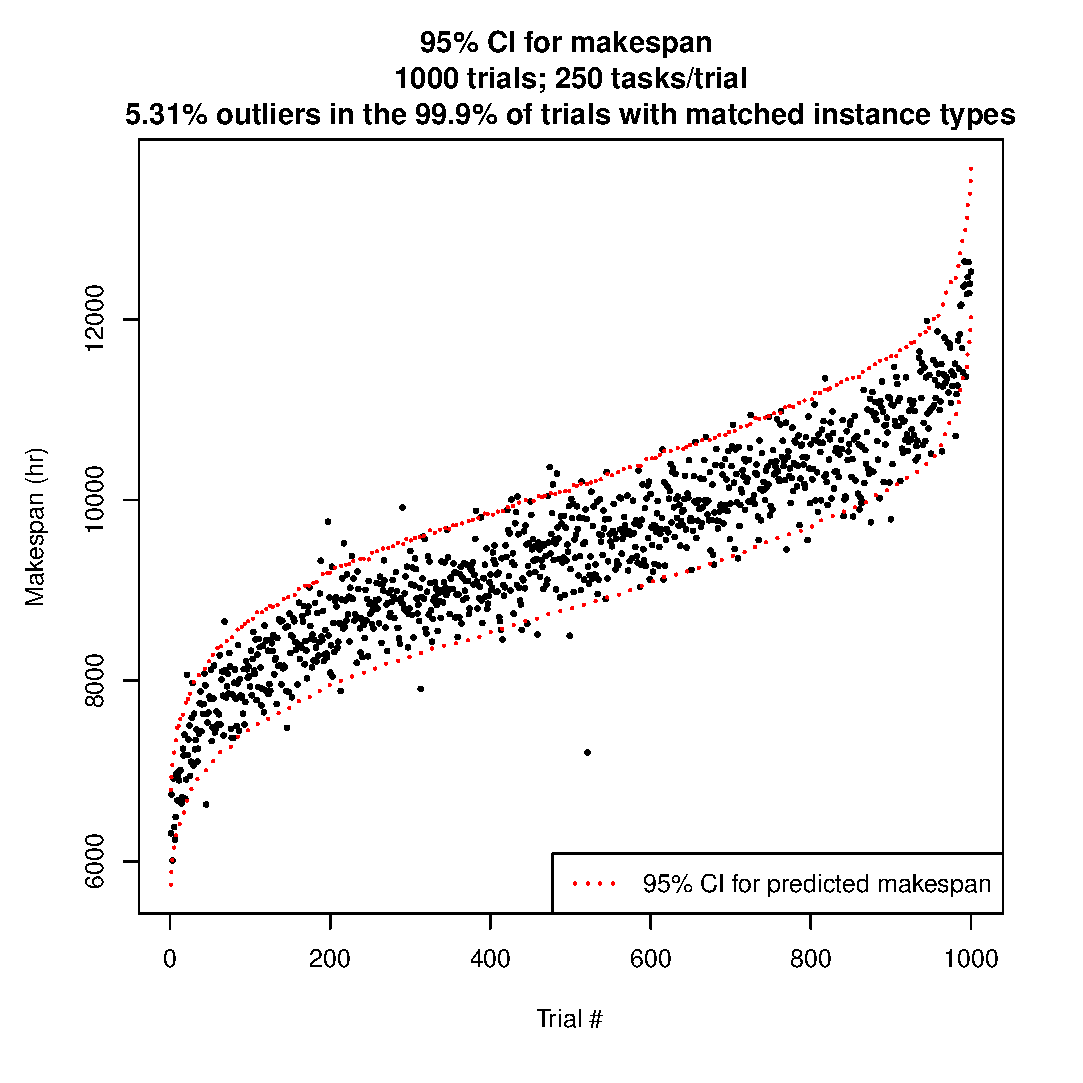
\includegraphics[width=1\textwidth]{validate-stochastic-runtimes-1000-trials-250-tasks.eps}
\caption{\textit{95\% confidence interval for makespan using Normal approximation when 250 tasks are processed on a single instance. Data sorted by lower bound of 95\% CI.}}
\label{fig:validate-stochastic-runtimes-1000-trials-250-tasks}
\end{figure}

\begin{figure}
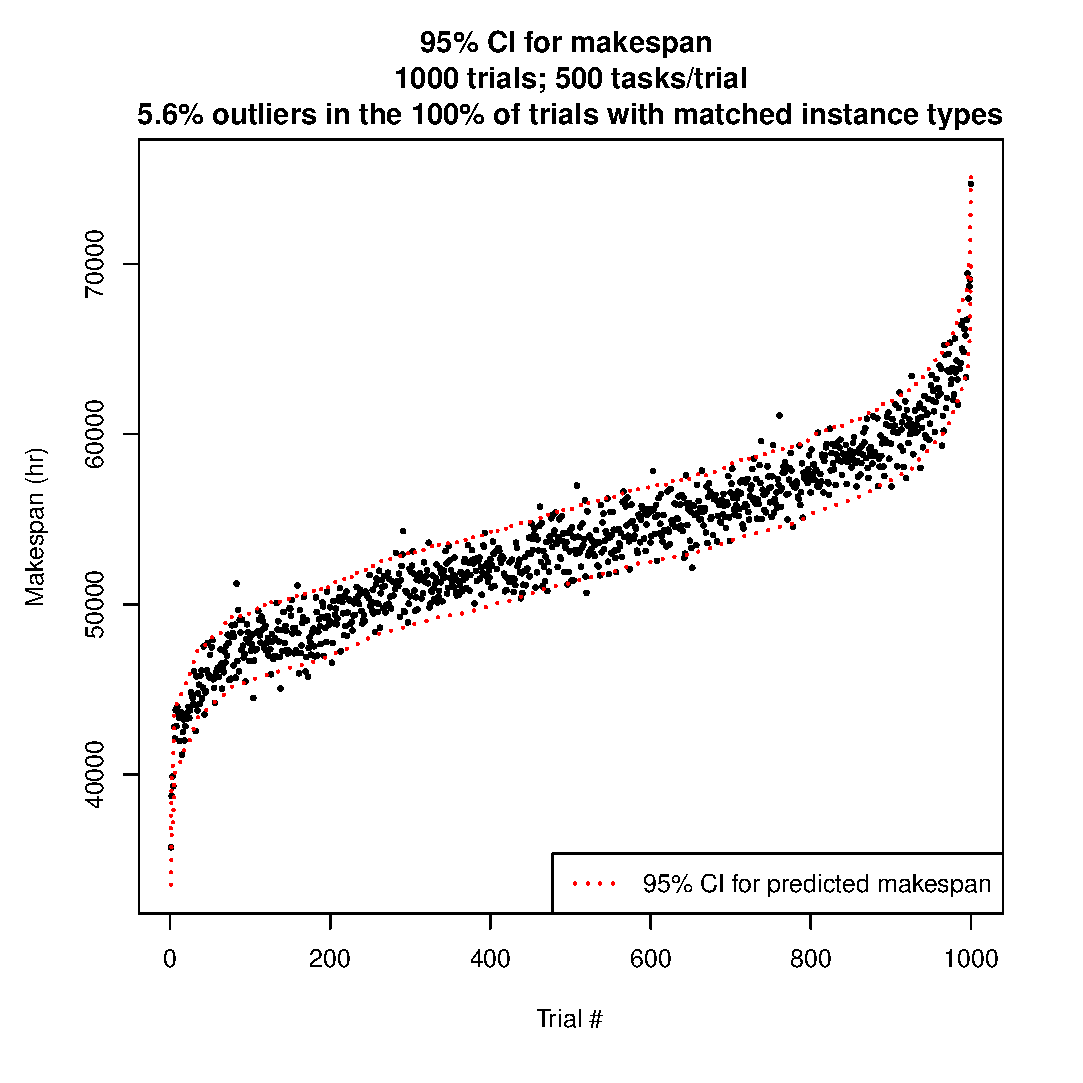
\includegraphics[width=1\textwidth]{validate-stochastic-runtimes-1000-trials-500-tasks.eps}
\caption{\textit{95\% confidence interval for makespan using Normal approximation when 500 tasks are processed on a single instance. Data sorted by lower bound of 95\% CI.}}
\label{fig:validate-stochastic-runtimes-1000-trials-500-tasks}
\end{figure}

\begin{figure}
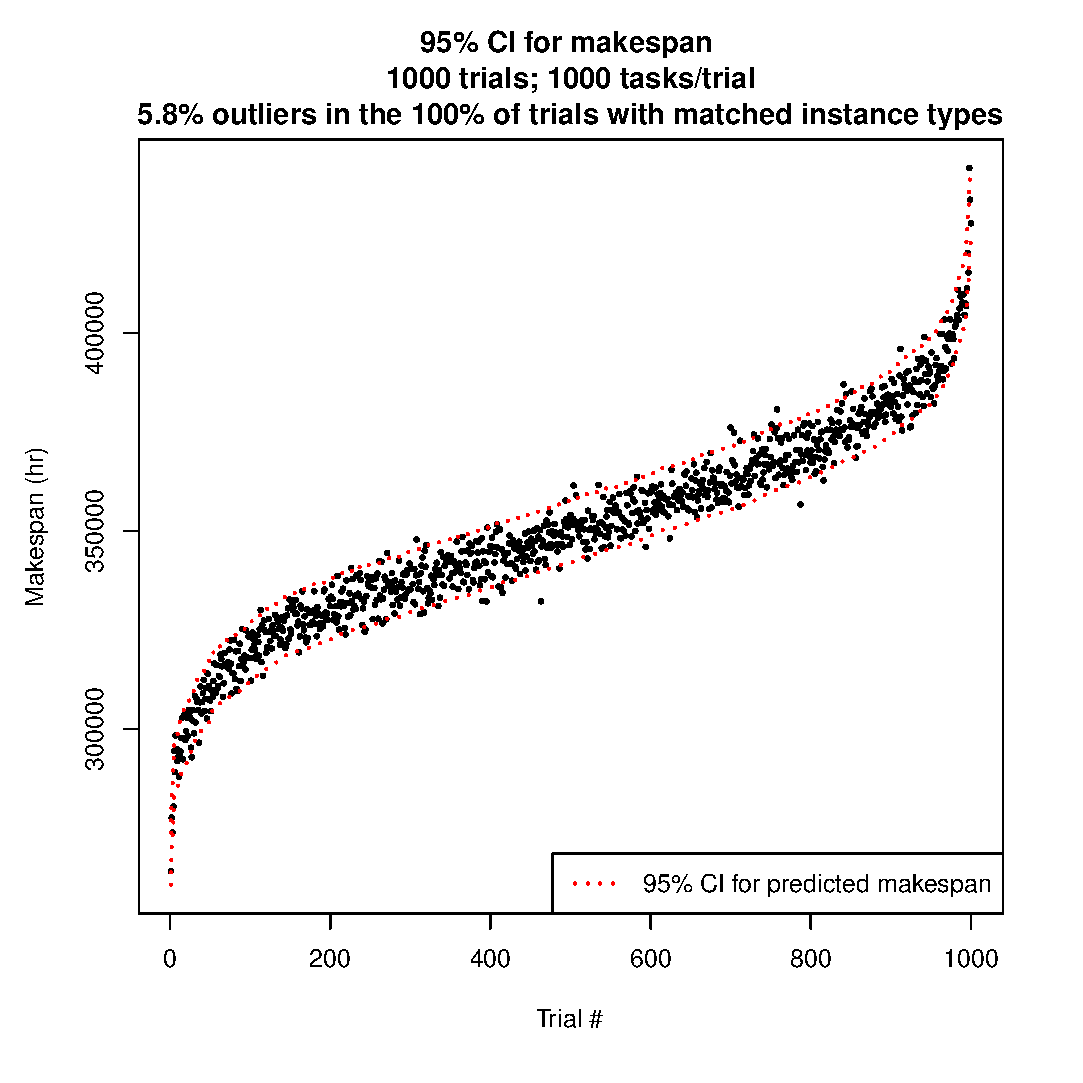
\includegraphics[width=1\textwidth]{validate-stochastic-runtimes-1000-trials-1000-tasks.eps}
\caption{\textit{95\% confidence interval for makespan using Normal approximation when 1000 tasks are processed on a single instance. Data sorted by lower bound of 95\% CI.}}
\label{fig:validate-stochastic-runtimes-1000-trials-1000-tasks}
\end{figure}


\subsection{$< 100$ tasks/instance}

When an instance is assigned less than 100 tasks/instance, the Central Limit Theorem does not apply and the makespan distribution must be determined through other means.
I use bootstrap re-sampling to construct a distribution for makespan.
Simulated collections of tasks are generated in the same manner as in the previous section and the predicted optimal schedules are compared to the true optimal schedules.

\begin{figure}
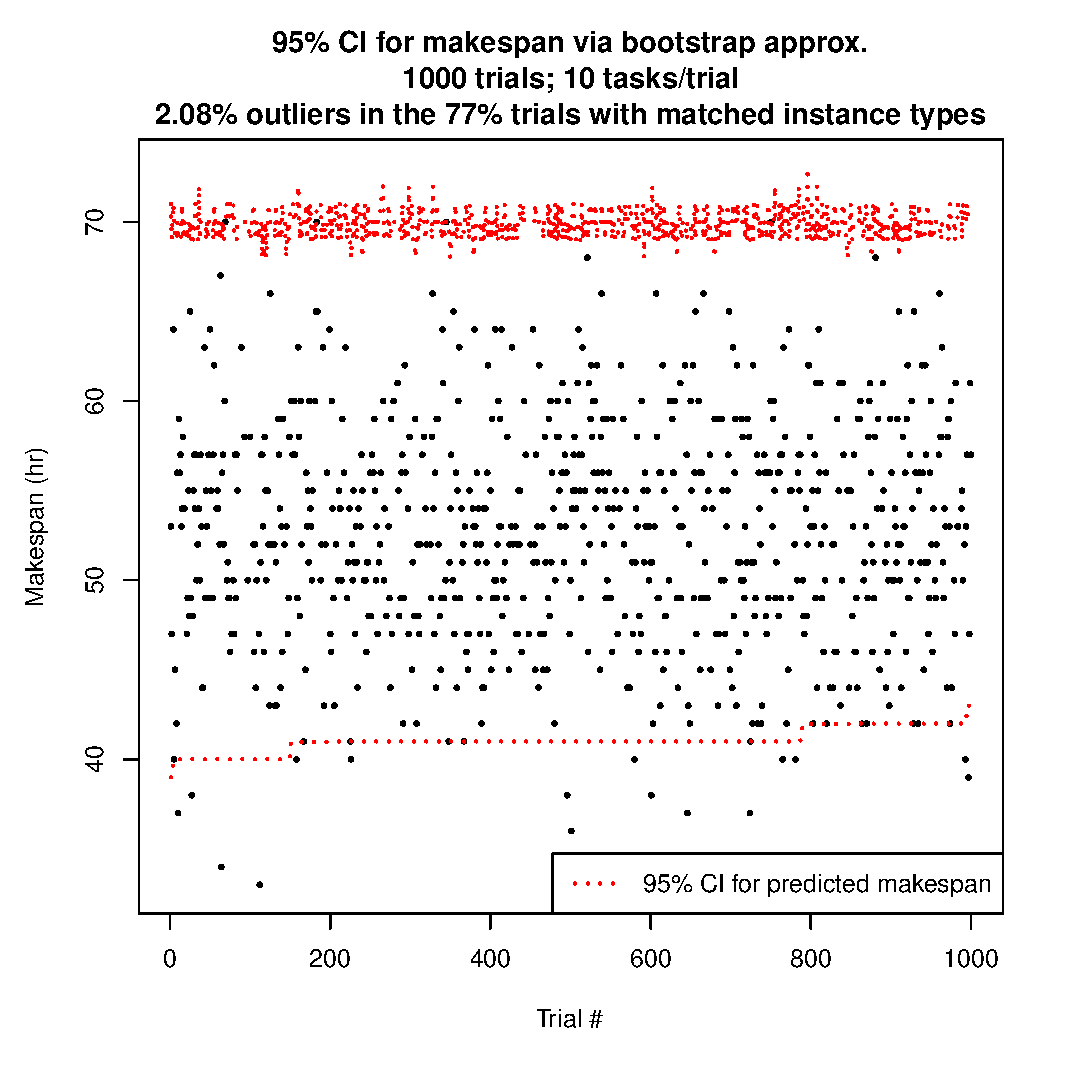
\includegraphics[width=1\textwidth]{validate-stochastic-runtimes-1000-trials-10-tasks.eps}
\caption{\textit{95\% confidence interval for makespan using Normal approximation when 10 tasks are processed on a single instance. Data sorted by lower bound of 95\% CI.}}
\label{fig:validate-stochastic-runtimes-1000-trials-10-tasks}
\end{figure}

\begin{figure}
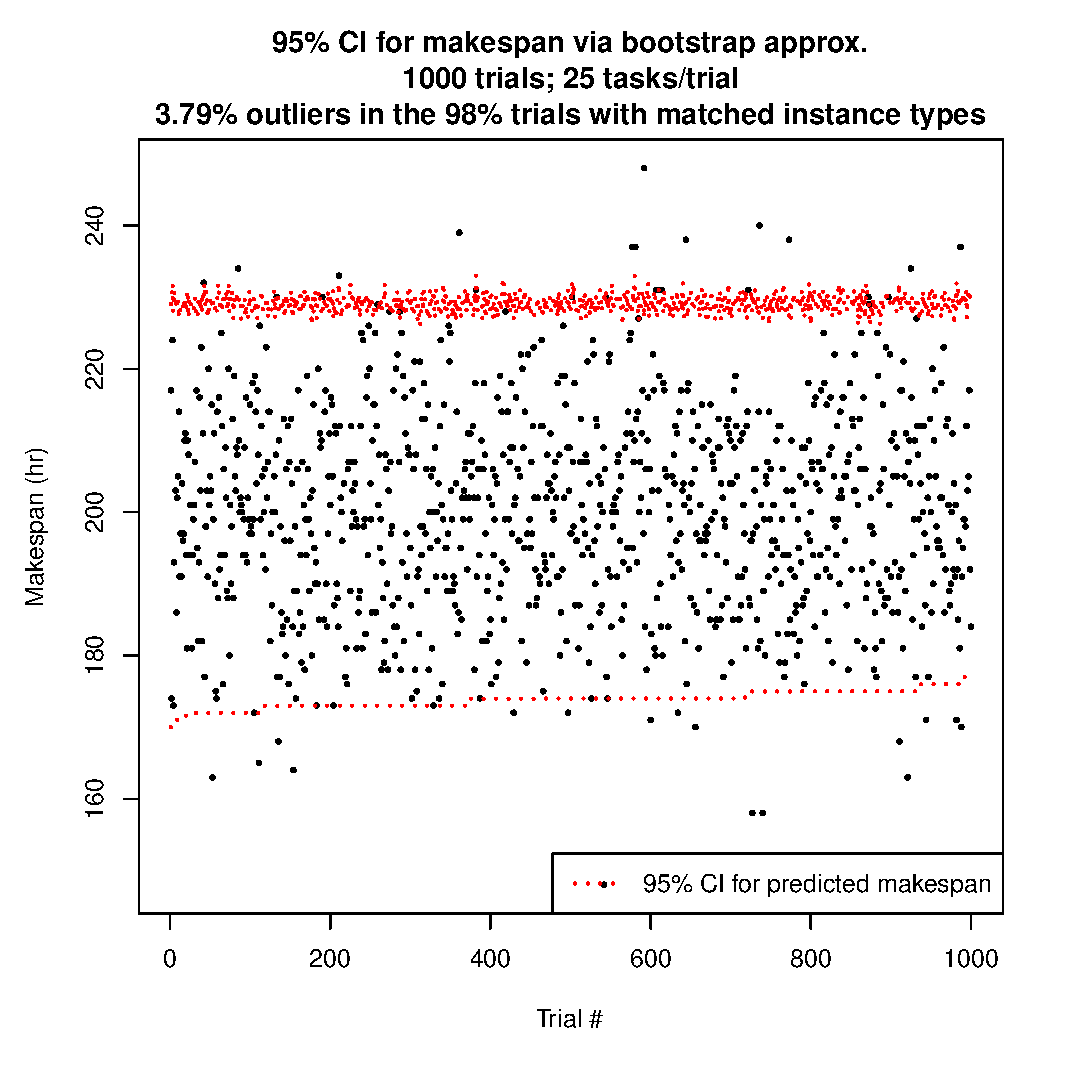
\includegraphics[width=1\textwidth]{validate-stochastic-runtimes-1000-trials-25-tasks.eps}
\caption{\textit{95\% confidence interval for makespan using Normal approximation when 25 tasks are processed on a single instance. Data sorted by lower bound of 95\% CI.}}
\label{fig:validate-stochastic-runtimes-1000-trials-25-tasks}
\end{figure}

\begin{figure}
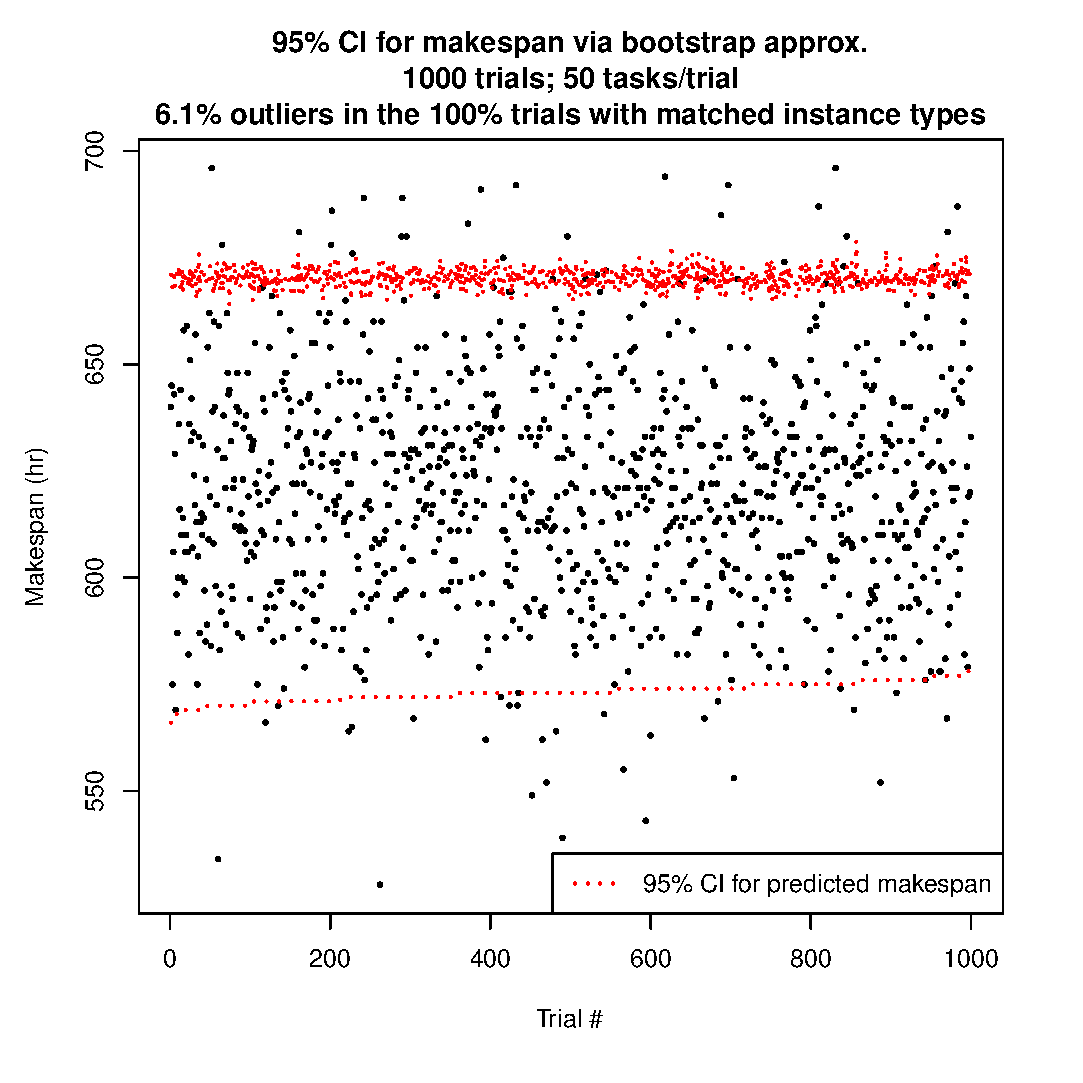
\includegraphics[width=1\textwidth]{validate-stochastic-runtimes-1000-trials-50-tasks.eps}
\caption{\textit{95\% confidence interval for makespan using Normal approximation when 50 tasks are processed on a single instance. Data sorted by lower bound of 95\% CI.}}
\label{fig:validate-stochastic-runtimes-1000-trials-50-tasks}
\end{figure}

\begin{figure}
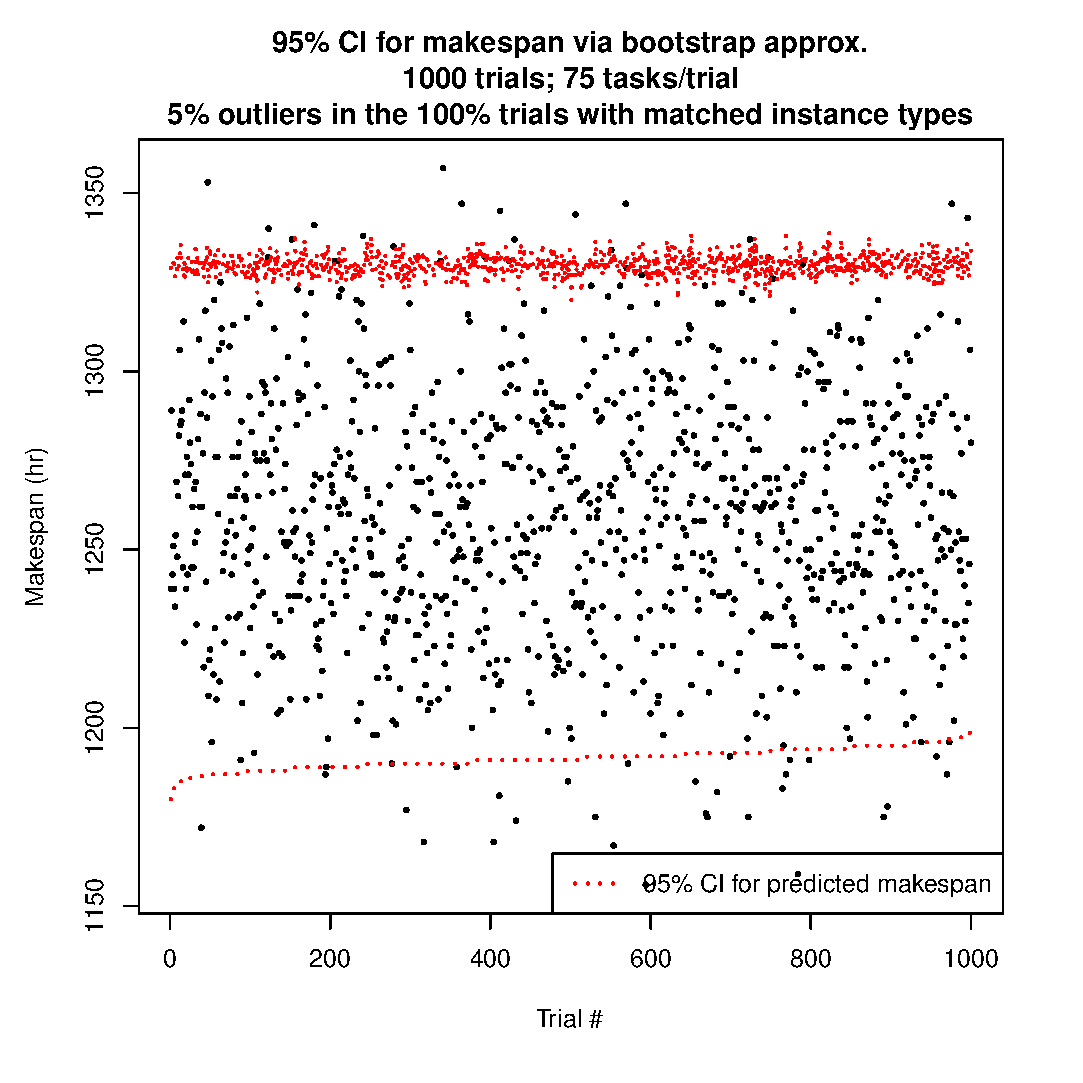
\includegraphics[width=1\textwidth]{validate-stochastic-runtimes-1000-trials-75-tasks.eps}
\caption{\textit{95\% confidence interval for makespan using Normal approximation when 75 tasks are processed on a single instance. Data sorted by lower bound of 95\% CI.}}ha
\label{fig:validate-stochastic-runtimes-1000-trials-75-tasks}
\end{figure}

Figure \ref{fig:validate-stochastic-runtimes-1000-trials-10-tasks} shows the 95\% confidence interval for makespan when 10 tasks are processed on a single instance. 
In this case, the predictions are not very good - only 77\% of the predictions use the optimal instance type.
Of this 77\%, the 95\% confidence interval contains all but 2.08\% of the true values of the makespan.
Figures \ref{fig:validate-stochastic-runtimes-1000-trials-25-tasks}, \ref{fig:validate-stochastic-runtimes-1000-trials-50-tasks} and \ref{fig:validate-stochastic-runtimes-1000-trials-75-tasks} show the corresponding confidence interval for 25, 50 and 75 tasks respectively. 
The results here are much better - almost all the predictions use the optimal instance type and the number of predictions outside the 95\% confidence interval is close to the error tolerance level of 5\%.
This means the total percentage of incorrect predictions is also close to 5\%.
The results suggest that predicting optimal schedules using bootstrap approximation is applicable only when at least 25 tasks are assigned to an instance and cannot be used when processing fewer number of tasks per instance.
Results (not shown) when sampling from empirical distributions for runtimes, rather than distributions with closed form expressions, are also very similar.

\section{Summary}
In this chapter I used two different methods to predict the optimal schedule when processing a tasks on a single machine. 
If the number of tasks is $>$ 100, the makespan distribution is approximated by a Normal approximation which is then used to predict optimal instance type and makespan. 
Prediction results are good and the percentage of incorrect prediction is around the error tolerance of 5\%. 
If the number of tasks is $\leq$ 100, then I use a bootstrap approximation to the makespan distribution and then the optimal schedule. 
Results using this method are poor when using $<$ 25 tasks/instance and improve only when processing at least 25 tasks/instance.
These methods form the core of the method used in the next section when scheduling tasks across multiple instances.

\chapter{The multiple instance case}

When scheduling tasks on single instances with the objective of minimizing makespan, there is only one possible schedule for each instance type.
When scheduling tasks on multiple instances, however, the number of possible schedules is typically very large and it is not possible to find the globally optimal schedule in a 'reasonable' amount of time.
In fact, most scheduling problems, including the problem of minimizing makespan, are considered to be NP-hard \cite{Garey1979} and form an important class of combinatorial problems.

A common algorithm to find a near-optimal schedule for deterministic runtimes when using multiple instances is called the Longest Processing Time First (LPTF) rule.
When runtimes are stochastic and follow the Exponential distribution, the Longest Expected Processing Time First (LEPTF) rule gives a near-optimal schedule \cite{Pinedo2012}. 
These rules first order all tasks in decreasing order of (expected) runtimes.
They then assign the task with the largest (expected) runtime that has not yet started processing to the next available instance. 
The schedule obtained by these rule has a makespan that is at most $\left(\frac{4}{3} - \frac{1}{3}m \right)$ greater than the makespan of the optimal schedule.

The proof of the near-optimality of the LEPTF rule relies on the memory-less property of the Exponential distribution, so this rule does not apply if the runtimes follow a different distribution.
In such cases, local search methods are used to find, in a 'reasonable' amount of time, a schedule that is 'close enough' to the global optimum.
Local search methods start with a candidate solution and explore all solutions in the \textit{neighborhood} of this solution \cite{Glass1994}.
If a \textit{better} solution is found, the search centers around the neighborhood of this solution.
This will ensure that the search is always moving toward the global optimum.
To avoid getting stuck in local optima, local search methods occasionally move to a \textit{worse} solution and explore the neighborhood around that solution in the hope of finding a path to the global optimum.

Fouskakis \cite{Fouskakis2001} compared several local search methods while trying to find the optimal set of predictors by trading off prediction accuracy against the cost of predictors. 
Simulated annealing, genetic algorithms, tabu search and their variants were compared and simulated annealing was found to perform better than other methods.
I chose sSimulated annealing as the local search method in this work based on its performance and the simplicity of its implementation.

\section{Method}

The steps involved in the simulated annealing (SA) algorithm to find the optimal schedule when runtimes are distributed according to an arbitrary distribution are described below:
\begin{itemize}
	\item \textbf{Initialization:} Select an initial feasible schedule as the current solution and compute its processing cost.
	\item \textbf{Candidate generation:} Generate a candidate schedule by moving or exchanging 1 or more tasks between 2 instances in the cluster being used to process tasks. 
		For deterministic, known runtimes, compute makespan as shown in Eq. \ref{eq:def:makespan} and the processing cost of this makespan.
		For stochastic runtimes, compute the 95th percentile of the makespan distribution using either the Normal approximation or bootstrap approximation to the makespan distribution as specified in Chapter 2 and the processing cost of this makespan. In both cases, makespan is computed for each instance in the set of instances being used to process tasks. The makespan of the candidate schedule is equal to the maximum of the makespans of the individual instances.
	\item \textbf{Acceptance:} If the makespan of the candidate schedule is greater than the deadline, the schedule is not feasible, so reject it.
		Else, calculate the processing cost for the candidate schedule.
		If this processing cost is less than the processing cost of the current schedule, accept the candidate schedule.
		Else, accept the candidate schedule with a probability inversely proportional to the ratio of its cost to the cost of the current schedule.
	\item \textbf{Termination:} Terminate if the maximum number of iterations has been reached. The feasible schedule with the lowest cost found so far is the approximate solution to the problem.
\end{itemize}

By proceeding as above for a suitably large number of iterations, I explore the search space of possible schedules and find a feasible schedule that is 'close enough' to the best feasible schedule. 
The number of iterations and the starting temperature are fixed in advance.
A linear \textit{cooling schedule} is used where the temperature decreases linearly with each iteration.
There is only 1 iteration at each temperature. 
While exploring the search space, it is possible for the SA algorithm to make a series of bad moves and end up with a schedule that is considerably worse than the initial schedule.
To prevent this, the above algorithm moves back to the best schedule determined so far whenever there is a 10\% increase in processing cost compared to the current best schedule.
This helps a lot with improving the efficiency of exploring the search space.
The above algorithm assumes that the number of instances is fixed.
It must be repeated for every combination of instance types and cluster size that I want to compare.

\section{Validation}

To validate the simulated annealing algorithm, I need a simulated data set where 'truth' is known.
Here I focus on the case when runtimes are distributed according to an unknown distribution and an empirical distribution for runtimes must be obtained.
I first define a set of 83 lengths that form a representative sample of the corresponding population, where lengths range from 1 to 3000.
Task runtimes are assumed to be exponentially distributed to facilitate comparison with results from the LEPTF rule mentioned in the previous section.
Since runtimes are roughly proportional to length, the parameters of the exponential distributions increase with length.
Distributions of runtimes for tasks with a smaller length will be shifted to the left compared to those for tasks with larger lengths.
For each of these lengths, I generated a set of 200 samples from an exponential distribution.
These samples represent the empirical distribution of runtimes for the set of input tasks. 
The SA algorithm only uses the empirical distributions and does not know that they are generated from exponential distributions.

To create a set of input tasks, I sampled with replacement 10 values from the set of 83 lengths.
I assume that these tasks will be processed on 2 instances of the same type and that the benefit and deadline are given.
The LEPTF rule is used to determine the near-optimal schedule for this set of tasks.
The SA algorithm is also used to predict the optimal schedule for the same set of tasks and the same 2 instances.
The probability of completing the tasks by the deadline and the cost of processing the tasks are calculated for both schedules.
This process is repeated for 100 sets of input tasks and the results are compared.

Figure \ref{fig:validate-SA-LEPT-scores-2inst-100iter-10tasks} shows the probability of completing the tasks by the deadline.
Note that all probabilities are rounded to 2 digits after the decimal point.
Schedules generated by the LEPTF rule in all 100 trials have at least 95\% probability of completing the tasks by the deadline.
Most of the schedules generated by the SA algorithm also have a $\geq 95\%$ chance of completing the tasks by the deadline.
But the probability for the schedules for a few trials is well below 95\%.
I attribute this to starting from a non-feasible solution with a low probability and being unable to find a feasible schedule within the given number of iterations.
This problem is usually remedied by starting from a feasible schedule.
Letting the SA algorithm run longer might also help find a better schedule.

Figure \ref{fig:validate-SA-LEPT-costs-2inst-100iter-10tasks} shows the costs associated with the same schedules. 
Costs for schedules generated by both methods are strongly correlated (Pearson correlation = 0.98).
But costs for SA schedules are almost uniformly lower than costs for the LEPTF for the same set of tasks.
This is unexpected since LEPTF generates the near-optimal schedule with the near-optimal cost while SA may not always generate the optimal schedule and I expect most of the points to be on or below the diagonal line.
I attribute this behavior to the size of the simulated data sets, each of which contains only 200 samples.

\begin{figure}
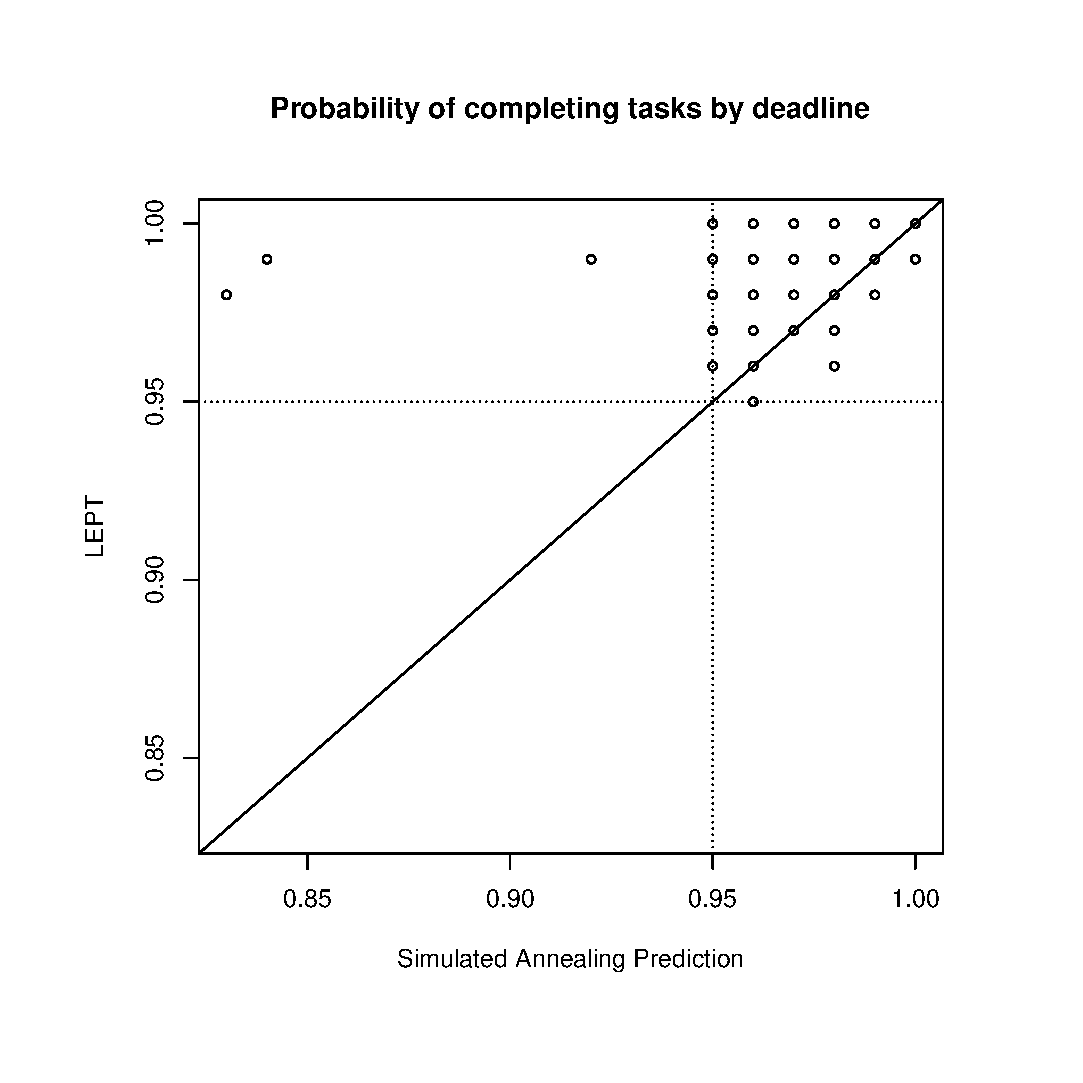
\includegraphics[width=1\textwidth]{validate-SA-LEPT-scores-2inst-100iter-10tasks.eps}
\caption{\textit{Probability of completing tasks by the deadline for schedules generated by the Simulated Annealing scheduling algorithm and the Longest Expected Processing Time First (LEPT) rule when runtimes are exponentially distributed.}}
\label{fig:validate-SA-LEPT-scores-2inst-100iter-10tasks}
\end{figure}

\begin{figure}
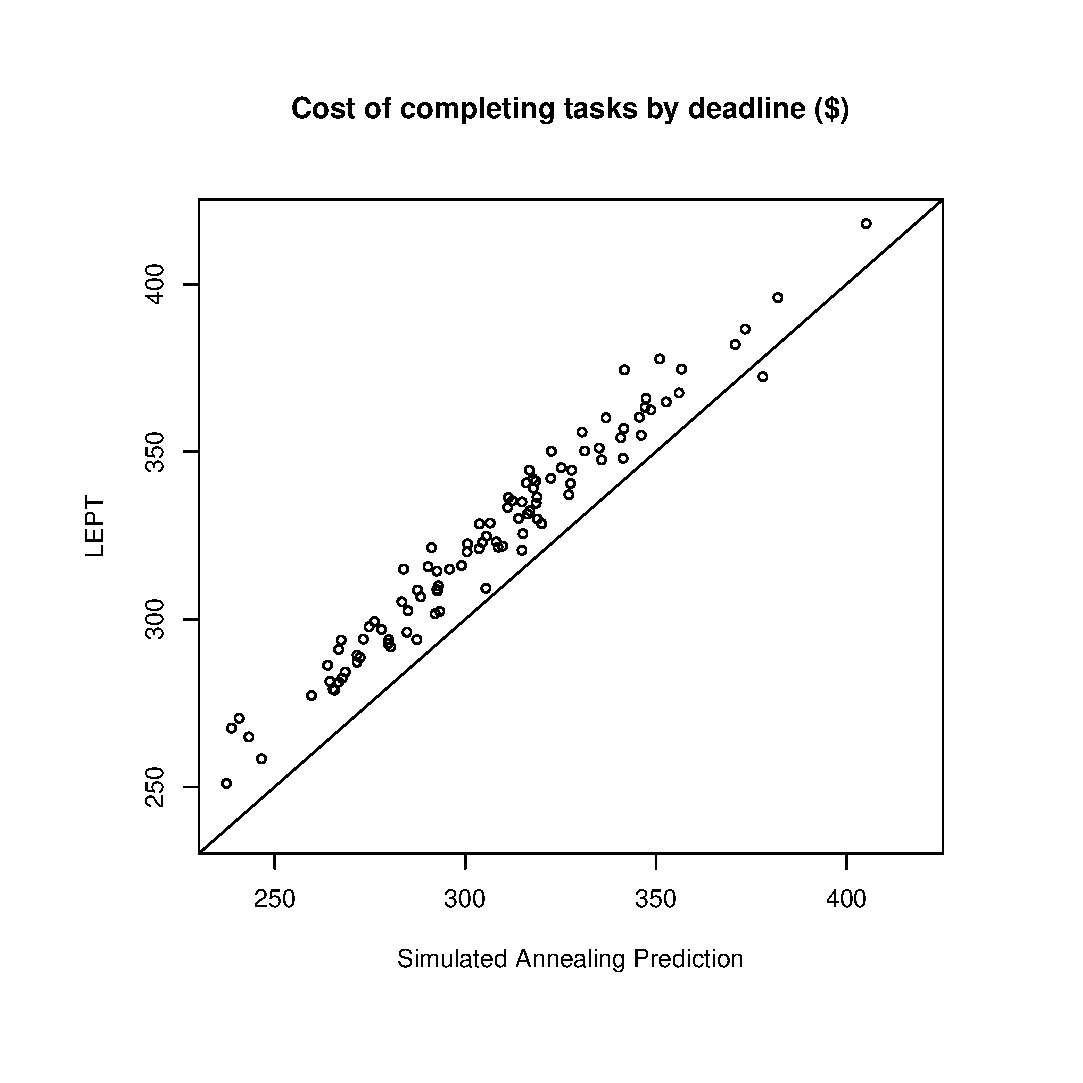
\includegraphics[width=1\textwidth]{validate-SA-LEPT-costs-2inst-100iter-10tasks.eps}
\caption{\textit{Cost of completing tasks by the deadline for schedules generated by the Simulated Annealing scheduling algorithm and the Longest Expected Processing Time First (LEPTF) rule when runtimes are exponentially distributed.}}
\label{fig:validate-SA-LEPT-costs-2inst-100iter-10tasks}
\end{figure}


\section{Summary}
This chapter described a method that uses Simulated Annealing to find the optimal feasible schedule for a set of tasks whose runtimes follow an unknown distribution.
The algorithm was validated using exponentially distributed runtimes and the schedules generated by the algorithm were compared to the corresponding schedules generated by the LEPTF rule.
The results were favorable with the percentage of sub-optimal schedules being under the error tolerance of 5\%.


\chapter{Conclusion and future work}

\section{Conclusion}

In this work I developed methods to find optimal schedules for tasks with stochastic runtimes. 
When processing tasks on a single instance, a Normal approximation or a bootstrap approximation to the makespan distribution was used depending on the number of tasks to be processed on the instance.
The $95th$ percentile of this makespan distribution was used to determine the optimal schedule.
The optimal schedule was predicted with 95\% accuracy for simulated data sets when at least 25 tasks were being processed on an instance. 
The percentage of sub-optimal predictions was around the error tolerance of 5\%. 
When processing tasks on multiple instances, simulated annealing was used to explore the search space of feasible schedules.
The results from the above method compared favorably to results from the LEPTF rule.

\section{Future work}

The methodology developed in the previous chapters can be extended in the following ways:

\begin{itemize}

	\item \textbf{Varying SA parameters:} Simulated annealing has several parameters that can be tuned to the problem at hand.
	Only a few parameters are explored in this work.
	Other parameters worth exploring include improved methods of candidate generation, skipping evaluation of small clusters of slow instances that have no chance of completing all tasks by the deadline, alternative cooling schedules, multiple iterations at the same temperature and re-starting the annealing process from the starting temperature after moving back to a previous solution. 
	Some of these options are discussed in Fouskakis \cite{Fouskakis2001}.
	
	\item \textbf{Using alternative stochastic local search methods:} 
	The simulated annealing algorithm \cite{Kirkpatrick1983} used in Chapter 3 for finding the optimal schedule is just one member of a class of algorithms known as meta-heuristics for solving combinatorial problems.
	Other members of this class include tabu search \cite{Glover1989, Glover1990}, genetic algorithms \cite{Holland1992}, Ant Colony Optimization \cite{Dorigo2006} and their variants \cite{Hoos2004}.
	Performing a comparison similar to the one done in Fouskakis \cite{Fouskakis2001} will determine if other methods perform better than simulated annealing.
	
	\item \textbf{Using variable instance cost:} An important assumption in this work (see Eq. \ref{eq:def:utility:deterministic}) is that the cost of the instance on which a task is being processed is fixed.
		Amazon Web Services has the concept of Spot Instances \cite{AWS:Spot}, where temporarily unused capacity is sold at deeply discounted prices (70-90\% off). 
		Customers name a maximum price they are willing to pay for an instance and retain the instance as long as the spot price remains below this maximum value.
		The spot price keeps fluctuating based on supply and demand and can vary a lot within the same hour, sometimes even going above the fixed price for the instance.
		This setup allows Amazon to earn income on idle capacity and gives customers a much cheaper way to process their tasks as long as they are willing to endure interruptions.
		Taking advantage of this feature requires the development of \textit{pre-emptive} schedules where tasks can be stopped and re-started later and the prediction of future Spot prices based on the most recent set of prices to determine the maximum bid that should be placed on instance price.
		The significant reduction of processing costs makes this a feature worth exploring further.
	
\end{itemize}


\newpage
\sloppy
\printbibliography

\appendix
\chapter{Code to generate the results in Chapters 2 and 3}

This is the code to generate the plots and tables in Chapters 2 and 3

\begin{Shaded}
\begin{Highlighting}[]
\KeywordTok{rm}\NormalTok{(}\DataTypeTok{list =} \KeywordTok{ls}\NormalTok{())}

\CommentTok{# Install devtools and use devtools to install schedulr from}
\CommentTok{# GitHub to run simulated annealing code. This is done only}
\CommentTok{# once for each new version of schedulr}
\CommentTok{# install.packages('devtools')}
\CommentTok{# devtools::install_github('niranjv/schedulr', ref='develop')}

\CommentTok{# load schedulr & setup exponential runtimes dataset}
\KeywordTok{library}\NormalTok{(schedulr)}

\KeywordTok{data}\NormalTok{(m3xlarge.runtimes.expdist)}
\NormalTok{data.env =}\StringTok{ }\KeywordTok{setup.trainingset.runtimes}\NormalTok{(}\StringTok{"m3xlarge"}\NormalTok{, m3xlarge.runtimes.expdist)}
\NormalTok{rt <-}\StringTok{ }\KeywordTok{get}\NormalTok{(}\StringTok{"m3xlarge.runtimes"}\NormalTok{, }\DataTypeTok{envir =} \NormalTok{data.env)}
\NormalTok{rts <-}\StringTok{ }\KeywordTok{get}\NormalTok{(}\StringTok{"m3xlarge.runtimes.summary"}\NormalTok{, }\DataTypeTok{envir =} \NormalTok{data.env)}


\CommentTok{# init vars}

\CommentTok{# assume 3 instance types available e.g., (m3.large, c3.large,}
\CommentTok{# c4.large) in AWS EC2 with: processing speed = (3.25, 3.5, 4)}
\CommentTok{# processing cost = (0.14, 0.105, 0.116)}
\NormalTok{instance.types <-}\StringTok{ }\KeywordTok{c}\NormalTok{(}\StringTok{"m3.large"}\NormalTok{, }\StringTok{"c3.large"}\NormalTok{, }\StringTok{"c4.large"}\NormalTok{)}
\NormalTok{instance.speed <-}\StringTok{ }\KeywordTok{c}\NormalTok{(}\FloatTok{3.25}\NormalTok{, }\FloatTok{3.5}\NormalTok{, }\DecValTok{4}\NormalTok{)}
\NormalTok{instance.costs <-}\StringTok{ }\KeywordTok{c}\NormalTok{(}\FloatTok{0.14}\NormalTok{, }\FloatTok{0.105}\NormalTok{, }\FloatTok{0.116}\NormalTok{)}


\CommentTok{#' Create validation dataset}
\CommentTok{#'}
\CommentTok{#' Runtime for each tasks can have a different distribution}
\CommentTok{#' Input array has the name of the distribution of the runtime for each task}
\CommentTok{#'}
\CommentTok{#' @param runtimes.dist Array of strings representing the distribution of}
\CommentTok{#' runtimes. Currently, the distributions must be one of}
\CommentTok{#' ('unif', 'poisson', 'gamma', 'exp').}
\CommentTok{#' @return A list containing the details of the distribution of runtimes for}
\CommentTok{#' each task in the input set of tasks}
\NormalTok{create.validation.data <-}\StringTok{ }\NormalTok{function(runtimes.dist) \{}
    
    \NormalTok{num.tasks <-}\StringTok{ }\KeywordTok{NROW}\NormalTok{(runtimes.dist)}
    \NormalTok{num.instance.types =}\StringTok{ }\KeywordTok{NROW}\NormalTok{(instance.types)}
    
    \NormalTok{simulated.runtimes <-}\StringTok{ }\KeywordTok{matrix}\NormalTok{(}\DataTypeTok{nrow =} \NormalTok{num.tasks, }\DataTypeTok{ncol =} \NormalTok{num.instance.types)}
    \KeywordTok{colnames}\NormalTok{(simulated.runtimes) <-}\StringTok{ }\KeywordTok{paste}\NormalTok{(}\StringTok{"runtimes."}\NormalTok{, instance.types, }
        \DataTypeTok{sep =} \StringTok{""}\NormalTok{)}
    
    \NormalTok{means <-}\StringTok{ }\KeywordTok{matrix}\NormalTok{(}\DataTypeTok{nrow =} \NormalTok{num.tasks, }\DataTypeTok{ncol =} \NormalTok{num.instance.types)}
    \NormalTok{vars <-}\StringTok{ }\KeywordTok{matrix}\NormalTok{(}\DataTypeTok{nrow =} \NormalTok{num.tasks, }\DataTypeTok{ncol =} \NormalTok{num.instance.types)}
    \NormalTok{dist.params <-}\StringTok{ }\KeywordTok{list}\NormalTok{()}
    
    \NormalTok{runtimes <-}\StringTok{ }\DecValTok{1} \NormalTok{+}\StringTok{ }\NormalTok{(}\DecValTok{1}\NormalTok{:}\KeywordTok{length}\NormalTok{(runtimes.dist))/}\DecValTok{60}  \CommentTok{# baseline for params}
    \NormalTok{for (i in }\DecValTok{1}\NormalTok{:}\KeywordTok{length}\NormalTok{(runtimes.dist)) \{}
        
        \NormalTok{param.a <-}\StringTok{ }\NormalTok{runtimes[i] *}\StringTok{ }\NormalTok{instance.speed[}\DecValTok{1}\NormalTok{]}
        \NormalTok{param.b <-}\StringTok{ }\NormalTok{runtimes[i] *}\StringTok{ }\NormalTok{instance.speed[}\DecValTok{2}\NormalTok{]}
        \NormalTok{param.c <-}\StringTok{ }\NormalTok{runtimes[i] *}\StringTok{ }\NormalTok{instance.speed[}\DecValTok{3}\NormalTok{]}
        
        \CommentTok{# Discrete Uniform}
        \NormalTok{if (runtimes.dist[i] ==}\StringTok{ "unif"}\NormalTok{) \{}
            
            \NormalTok{means[i, }\DecValTok{1}\NormalTok{] <-}\StringTok{ }\NormalTok{(}\DecValTok{1} \NormalTok{+}\StringTok{ }\NormalTok{param.a)/}\DecValTok{2}
            \NormalTok{means[i, }\DecValTok{2}\NormalTok{] <-}\StringTok{ }\NormalTok{(}\DecValTok{1} \NormalTok{+}\StringTok{ }\NormalTok{param.b)/}\DecValTok{2}
            \NormalTok{means[i, }\DecValTok{3}\NormalTok{] <-}\StringTok{ }\NormalTok{(}\DecValTok{1} \NormalTok{+}\StringTok{ }\NormalTok{param.c)/}\DecValTok{2}
            
            \NormalTok{simulated.runtimes[i, }\DecValTok{1}\NormalTok{] <-}\StringTok{ }\KeywordTok{runif}\NormalTok{(}\DecValTok{1}\NormalTok{, }\DecValTok{1}\NormalTok{, param.a)}
            \NormalTok{simulated.runtimes[i, }\DecValTok{2}\NormalTok{] <-}\StringTok{ }\KeywordTok{runif}\NormalTok{(}\DecValTok{1}\NormalTok{, }\DecValTok{1}\NormalTok{, param.b)}
            \NormalTok{simulated.runtimes[i, }\DecValTok{3}\NormalTok{] <-}\StringTok{ }\KeywordTok{runif}\NormalTok{(}\DecValTok{1}\NormalTok{, }\DecValTok{1}\NormalTok{, param.c)}
            
            \NormalTok{vars[i, }\DecValTok{1}\NormalTok{] <-}\StringTok{ }\NormalTok{((param.a -}\StringTok{ }\DecValTok{1}\NormalTok{)^}\DecValTok{2}\NormalTok{)/}\DecValTok{12}
            \NormalTok{vars[i, }\DecValTok{2}\NormalTok{] <-}\StringTok{ }\NormalTok{((param.b -}\StringTok{ }\DecValTok{1}\NormalTok{)^}\DecValTok{2}\NormalTok{)/}\DecValTok{12}
            \NormalTok{vars[i, }\DecValTok{3}\NormalTok{] <-}\StringTok{ }\NormalTok{((param.c -}\StringTok{ }\DecValTok{1}\NormalTok{)^}\DecValTok{2}\NormalTok{)/}\DecValTok{12}
            
            \NormalTok{dist.params[[i]] <-}\StringTok{ }\KeywordTok{list}\NormalTok{(}\DataTypeTok{dist =} \StringTok{"unif"}\NormalTok{, }\DataTypeTok{params =} \KeywordTok{c}\NormalTok{(param.a, }
                \NormalTok{param.b, param.c))}
        \NormalTok{\}}
        
        \CommentTok{# Gamma}
        \NormalTok{if (runtimes.dist[i] ==}\StringTok{ "gamma"}\NormalTok{) \{}
            
            \NormalTok{means[i, }\DecValTok{1}\NormalTok{] <-}\StringTok{ }\NormalTok{param.a^}\DecValTok{2}
            \NormalTok{means[i, }\DecValTok{2}\NormalTok{] <-}\StringTok{ }\NormalTok{param.b^}\DecValTok{2}
            \NormalTok{means[i, }\DecValTok{3}\NormalTok{] <-}\StringTok{ }\NormalTok{param.c^}\DecValTok{2}
            
            \NormalTok{simulated.runtimes[i, }\DecValTok{1}\NormalTok{] <-}\StringTok{ }\KeywordTok{rgamma}\NormalTok{(}\DecValTok{1}\NormalTok{, }\DataTypeTok{shape =} \NormalTok{param.a, }
                \DataTypeTok{scale =} \NormalTok{param.a)}
            \NormalTok{simulated.runtimes[i, }\DecValTok{2}\NormalTok{] <-}\StringTok{ }\KeywordTok{rgamma}\NormalTok{(}\DecValTok{1}\NormalTok{, }\DataTypeTok{shape =} \NormalTok{param.b, }
                \DataTypeTok{scale =} \NormalTok{param.b)}
            \NormalTok{simulated.runtimes[i, }\DecValTok{3}\NormalTok{] <-}\StringTok{ }\KeywordTok{rgamma}\NormalTok{(}\DecValTok{1}\NormalTok{, }\DataTypeTok{shape =} \NormalTok{param.c, }
                \DataTypeTok{scale =} \NormalTok{param.c)}
            
            \NormalTok{vars[i, }\DecValTok{1}\NormalTok{] <-}\StringTok{ }\NormalTok{param.a^}\DecValTok{3}
            \NormalTok{vars[i, }\DecValTok{2}\NormalTok{] <-}\StringTok{ }\NormalTok{param.b^}\DecValTok{3}
            \NormalTok{vars[i, }\DecValTok{3}\NormalTok{] <-}\StringTok{ }\NormalTok{param.c^}\DecValTok{3}
            
            \NormalTok{dist.params[[i]] <-}\StringTok{ }\KeywordTok{list}\NormalTok{(}\DataTypeTok{dist =} \StringTok{"gamma"}\NormalTok{, }\DataTypeTok{params =} \KeywordTok{c}\NormalTok{(param.a, }
                \NormalTok{param.b, param.c))}
        \NormalTok{\}}
        
        \CommentTok{# Poisson}
        \NormalTok{if (runtimes.dist[i] ==}\StringTok{ "poisson"}\NormalTok{) \{}
            
            \NormalTok{param.a <-}\StringTok{ }\KeywordTok{round}\NormalTok{(param.a)}
            \NormalTok{param.b <-}\StringTok{ }\KeywordTok{round}\NormalTok{(param.b)}
            \NormalTok{param.c <-}\StringTok{ }\KeywordTok{round}\NormalTok{(param.c)}
            
            \NormalTok{means[i, }\DecValTok{1}\NormalTok{] <-}\StringTok{ }\NormalTok{param.a}
            \NormalTok{means[i, }\DecValTok{2}\NormalTok{] <-}\StringTok{ }\NormalTok{param.b}
            \NormalTok{means[i, }\DecValTok{3}\NormalTok{] <-}\StringTok{ }\NormalTok{param.c}
            
            \NormalTok{simulated.runtimes[i, }\DecValTok{1}\NormalTok{] <-}\StringTok{ }\KeywordTok{rpois}\NormalTok{(}\DecValTok{1}\NormalTok{, param.a)}
            \NormalTok{simulated.runtimes[i, }\DecValTok{2}\NormalTok{] <-}\StringTok{ }\KeywordTok{rpois}\NormalTok{(}\DecValTok{1}\NormalTok{, param.b)}
            \NormalTok{simulated.runtimes[i, }\DecValTok{3}\NormalTok{] <-}\StringTok{ }\KeywordTok{rpois}\NormalTok{(}\DecValTok{1}\NormalTok{, param.c)}
            
            \NormalTok{vars[i, }\DecValTok{1}\NormalTok{] <-}\StringTok{ }\NormalTok{param.a}
            \NormalTok{vars[i, }\DecValTok{2}\NormalTok{] <-}\StringTok{ }\NormalTok{param.b}
            \NormalTok{vars[i, }\DecValTok{3}\NormalTok{] <-}\StringTok{ }\NormalTok{param.c}
            
            \NormalTok{dist.params[[i]] <-}\StringTok{ }\KeywordTok{list}\NormalTok{(}\DataTypeTok{dist =} \StringTok{"poisson"}\NormalTok{, }\DataTypeTok{params =} \KeywordTok{c}\NormalTok{(param.a, }
                \NormalTok{param.b, param.c))}
        \NormalTok{\}}
        
        \CommentTok{# Exponential}
        \NormalTok{if (runtimes.dist[i] ==}\StringTok{ "exp"}\NormalTok{) \{}
            
            \NormalTok{means[i, }\DecValTok{1}\NormalTok{] <-}\StringTok{ }\DecValTok{1}\NormalTok{/param.a}
            \NormalTok{means[i, }\DecValTok{2}\NormalTok{] <-}\StringTok{ }\DecValTok{1}\NormalTok{/param.b}
            \NormalTok{means[i, }\DecValTok{3}\NormalTok{] <-}\StringTok{ }\DecValTok{1}\NormalTok{/param.c}
            
            \NormalTok{simulated.runtimes[i, }\DecValTok{1}\NormalTok{] <-}\StringTok{ }\KeywordTok{rexp}\NormalTok{(}\DecValTok{1}\NormalTok{, param.a)}
            \NormalTok{simulated.runtimes[i, }\DecValTok{2}\NormalTok{] <-}\StringTok{ }\KeywordTok{rexp}\NormalTok{(}\DecValTok{1}\NormalTok{, param.b)}
            \NormalTok{simulated.runtimes[i, }\DecValTok{3}\NormalTok{] <-}\StringTok{ }\KeywordTok{rexp}\NormalTok{(}\DecValTok{1}\NormalTok{, param.c)}
            
            \NormalTok{vars[i, }\DecValTok{1}\NormalTok{] <-}\StringTok{ }\DecValTok{1}\NormalTok{/(param.a^}\DecValTok{2}\NormalTok{)}
            \NormalTok{vars[i, }\DecValTok{2}\NormalTok{] <-}\StringTok{ }\DecValTok{1}\NormalTok{/(param.b^}\DecValTok{2}\NormalTok{)}
            \NormalTok{vars[i, }\DecValTok{3}\NormalTok{] <-}\StringTok{ }\DecValTok{1}\NormalTok{/(param.c^}\DecValTok{2}\NormalTok{)}
            
            \NormalTok{dist.params[[i]] <-}\StringTok{ }\KeywordTok{list}\NormalTok{(}\DataTypeTok{dist =} \StringTok{"exp"}\NormalTok{, }\DataTypeTok{params =} \KeywordTok{c}\NormalTok{(param.a, }
                \NormalTok{param.b, param.c))}
        \NormalTok{\}}
    \NormalTok{\}}
    
    \KeywordTok{return}\NormalTok{(}\KeywordTok{list}\NormalTok{(}\DataTypeTok{simulated.runtimes =} \NormalTok{simulated.runtimes, }\DataTypeTok{means =} \NormalTok{means, }
        \DataTypeTok{vars =} \NormalTok{vars, }\DataTypeTok{dist.params =} \NormalTok{dist.params))}
    
\NormalTok{\}  }\CommentTok{# end function - create.validation.data}


\CommentTok{#' Calculate makespan for deterministic runtimes}
\CommentTok{#'}
\CommentTok{#' For deterministic runtimes, load is the sum of runtimes of tasks assigned}
\CommentTok{#' to an instance and makespan is the max of load across all instances.}
\CommentTok{#'}
\CommentTok{#' @param instance.types Array of instance types under consideration}
\CommentTok{#' @param instance.costs Array of cost per hour for above instance types}
\CommentTok{#' @param benefit Benefit of completing all tasks by deadline}
\CommentTok{#' @param deadline Time by which all costs must be complete}
\CommentTok{#' @param runtimes Deterministic runtimes for all tasks for all instance types}
\CommentTok{#' @return A list containing the maximum utility and the instance type and}
\CommentTok{#' makespan associated with this utility}
\NormalTok{get.schedule.deterministic.runtimes <-}\StringTok{ }\NormalTok{function(instance.types, }
    \NormalTok{instance.costs, benefit, deadline, runtimes) \{}
    
    \NormalTok{makespan <-}\StringTok{ }\KeywordTok{ceiling}\NormalTok{(}\KeywordTok{apply}\NormalTok{(runtimes, }\DecValTok{2}\NormalTok{, sum))}
    \NormalTok{makespan.feasible <-}\StringTok{ }\NormalTok{makespan[makespan <=}\StringTok{ }\NormalTok{deadline]}
    \NormalTok{instance.costs.feasible <-}\StringTok{ }\NormalTok{instance.costs[makespan <=}\StringTok{ }\NormalTok{deadline]}
    \NormalTok{instance.types.feasible <-}\StringTok{ }\NormalTok{instance.types[makespan <=}\StringTok{ }\NormalTok{deadline]}
    
    \NormalTok{util.feasible <-}\StringTok{ }\NormalTok{benefit -}\StringTok{ }\NormalTok{(instance.costs.feasible *}\StringTok{ }\NormalTok{makespan.feasible)}
    \NormalTok{max.util.idx <-}\StringTok{ }\KeywordTok{which.max}\NormalTok{(util.feasible)}
    \NormalTok{max.util <-}\StringTok{ }\NormalTok{util.feasible[max.util.idx]}
    \NormalTok{max.util.instance.type <-}\StringTok{ }\NormalTok{instance.types.feasible[max.util.idx]}
    \NormalTok{max.util.makespan <-}\StringTok{ }\NormalTok{makespan.feasible[max.util.idx]}
    
    \KeywordTok{return}\NormalTok{(}\KeywordTok{list}\NormalTok{(}\DataTypeTok{max.util =} \NormalTok{max.util, }\DataTypeTok{max.util.instance.type =} \NormalTok{max.util.instance.type, }
        \DataTypeTok{max.util.makespan =} \NormalTok{max.util.makespan))}
    
\NormalTok{\}  }\CommentTok{# end function - get.schedule.deterministic.runtimes}


\CommentTok{#' Calculate schedule for large number of tasks whose runtimes are distributed}
\CommentTok{#' according to known distributions}
\CommentTok{#'}
\CommentTok{#' @param instance.types Array of instance types under consideration}
\CommentTok{#' @param instance.costs Array of cost per hour for above instance types}
\CommentTok{#' @param benefit Benefit of completing all tasks by deadline}
\CommentTok{#' @param deadline Time by which all costs must be complete}
\CommentTok{#' @param means Array of means of runtime distributions}
\CommentTok{#' @param vars Array of variances of runtime distributions}
\CommentTok{#' @param feasible.pctl Percentile of makespan distribution. A schedule is }
\CommentTok{#' feasible only if the deadline is greater than this percentile of the }
\CommentTok{#' makespan distribution}
\CommentTok{#' @return A list containing the maximum utility, instance type and details of }
\CommentTok{#' the makespan associated with this utility}
\NormalTok{get.schedule.stochastic.runtimes <-}\StringTok{ }\NormalTok{function(instance.types, instance.costs, }
    \NormalTok{benefit, deadline, means, vars, feasible.pctl) \{}
    
    \KeywordTok{stopifnot}\NormalTok{(}\KeywordTok{dim}\NormalTok{(means) ==}\StringTok{ }\KeywordTok{dim}\NormalTok{(vars))}
    
    \NormalTok{means.sum <-}\StringTok{ }\KeywordTok{apply}\NormalTok{(means, }\DecValTok{2}\NormalTok{, sum)}
    \NormalTok{vars.sum <-}\StringTok{ }\KeywordTok{apply}\NormalTok{(vars, }\DecValTok{2}\NormalTok{, sum)}
    \NormalTok{sds <-}\StringTok{ }\KeywordTok{sqrt}\NormalTok{(vars.sum)}
    
    \NormalTok{makespan.pctl <-}\StringTok{ }\KeywordTok{qnorm}\NormalTok{(feasible.pctl, means.sum, sds)}
    \NormalTok{makespan.pctl <-}\StringTok{ }\KeywordTok{ceiling}\NormalTok{(makespan.pctl)}
    
    \NormalTok{feasible.idx <-}\StringTok{ }\NormalTok{makespan.pctl <=}\StringTok{ }\NormalTok{deadline}
    \NormalTok{makespan.feasible <-}\StringTok{ }\NormalTok{makespan.pctl[feasible.idx]}
    \NormalTok{instance.cost.feasible <-}\StringTok{ }\NormalTok{instance.costs[feasible.idx]}
    \NormalTok{instance.types.feasible <-}\StringTok{ }\NormalTok{instance.types[feasible.idx]}
    
    \NormalTok{util.feasible <-}\StringTok{ }\NormalTok{benefit -}\StringTok{ }\NormalTok{(instance.cost.feasible *}\StringTok{ }\NormalTok{makespan.feasible)}
    \NormalTok{max.util <-}\StringTok{ }\KeywordTok{max}\NormalTok{(util.feasible)}
    \NormalTok{max.util.idx <-}\StringTok{ }\KeywordTok{which.max}\NormalTok{(util.feasible)}
    
    \NormalTok{max.util.instance.type <-}\StringTok{ }\NormalTok{instance.types.feasible[max.util.idx]}
    \NormalTok{max.util.makespan.feasible.pctl <-}\StringTok{ }\NormalTok{makespan.feasible[max.util.idx]}
    
    \CommentTok{# assuming we are summing over enough tasks that the makespn}
    \CommentTok{# dist. is Normal}
    \NormalTok{max.util.makespan.mean <-}\StringTok{ }\NormalTok{means.sum[max.util.idx]}
    \NormalTok{max.util.makespan.sd <-}\StringTok{ }\NormalTok{sds[max.util.idx]}
    \NormalTok{max.util.makespan.lo <-}\StringTok{ }\NormalTok{max.util.makespan.mean -}\StringTok{ }\FloatTok{1.96} \NormalTok{*}\StringTok{ }\NormalTok{max.util.makespan.sd}
    \NormalTok{max.util.makespan.hi <-}\StringTok{ }\NormalTok{max.util.makespan.mean +}\StringTok{ }\FloatTok{1.96} \NormalTok{*}\StringTok{ }\NormalTok{max.util.makespan.sd}
    
    \KeywordTok{return}\NormalTok{(}\KeywordTok{list}\NormalTok{(}\DataTypeTok{max.util =} \NormalTok{max.util, }\DataTypeTok{max.util.instance.type =} \NormalTok{max.util.instance.type, }
        \DataTypeTok{max.util.makespan.feasible.pctl =} \NormalTok{max.util.makespan.feasible.pctl, }
        \DataTypeTok{max.util.makespan.mean =} \NormalTok{max.util.makespan.mean, }\DataTypeTok{max.util.makespan.lo =} \NormalTok{max.util.makespan.lo, }
        \DataTypeTok{max.util.makespan.hi =} \NormalTok{max.util.makespan.hi))}
    
\NormalTok{\}  }\CommentTok{# end function - get.schedule.stochastic.runtimes}


\CommentTok{#' Get validation results when makespan distributions are Normally distributed}
\CommentTok{#'}
\CommentTok{#' @param instance.types Array of instance types under consideration}
\CommentTok{#' @param instance.costs Array of cost per hour for above instance types}
\CommentTok{#' @param feasible.pctl Percentile of makespan distribution. A schedule is }
\CommentTok{#' feasible only if the deadline is greater than this percentile of the }
\CommentTok{#' makespan distribution}
\CommentTok{#' @param num.tasks Number of input tasks}
\CommentTok{#' @param num.trials Number of simulated data sets to process}
\CommentTok{#' @return Nothing. This function generates a plot as a side-effect}
\NormalTok{validate.stochastic.runtimes <-}\StringTok{ }\NormalTok{function(instance.types, instance.costs, }
    \DataTypeTok{feasible.pctl =} \FloatTok{0.95}\NormalTok{, num.tasks, }\DataTypeTok{num.trials =} \DecValTok{1000}\NormalTok{) \{}
    
    \NormalTok{validation.results <-}\StringTok{ }\KeywordTok{data.frame}\NormalTok{()}
    
    \NormalTok{for (j in }\DecValTok{1}\NormalTok{:num.trials) \{}
        
        \CommentTok{# cat('Processing iteration', j, '\textbackslash{}n')}
        
        \NormalTok{dist <-}\StringTok{ }\KeywordTok{c}\NormalTok{(}\StringTok{"unif"}\NormalTok{, }\StringTok{"poisson"}\NormalTok{, }\StringTok{"gamma"}\NormalTok{, }\StringTok{"exp"}\NormalTok{)}
        \NormalTok{runtimes.dist <-}\StringTok{ }\KeywordTok{sample}\NormalTok{(dist, num.tasks, }\DataTypeTok{replace =} \NormalTok{T)}
        \NormalTok{validation.data <-}\StringTok{ }\KeywordTok{create.validation.data}\NormalTok{(runtimes.dist)}
        
        \CommentTok{# a realistic benefit & deadline or no schedule will be found}
        \NormalTok{deadline =}\StringTok{ }\KeywordTok{round}\NormalTok{(}\DecValTok{4} \NormalTok{*}\StringTok{ }\KeywordTok{sum}\NormalTok{(validation.data$simulated.runtimes[, }
            \DecValTok{1}\NormalTok{]))}
        \NormalTok{benefit =}\StringTok{ }\NormalTok{deadline}
        
        \NormalTok{result.actual =}\StringTok{ }\KeywordTok{get.schedule.deterministic.runtimes}\NormalTok{(instance.types, }
            \NormalTok{instance.costs, benefit, deadline, validation.data$simulated.runtimes)}
        
        \NormalTok{result.predicted =}\StringTok{ }\KeywordTok{get.schedule.stochastic.runtimes}\NormalTok{(instance.types, }
            \NormalTok{instance.costs, benefit, deadline, validation.data$means, }
            \NormalTok{validation.data$vars, feasible.pctl)}
        
        \NormalTok{validation.results[j, }\DecValTok{1}\NormalTok{] <-}\StringTok{ }\NormalTok{result.actual$max.util}
        \NormalTok{validation.results[j, }\DecValTok{2}\NormalTok{] <-}\StringTok{ }\NormalTok{result.actual$max.util.instance.type}
        \NormalTok{validation.results[j, }\DecValTok{3}\NormalTok{] <-}\StringTok{ }\NormalTok{result.actual$max.util.makespan}
        
        \NormalTok{validation.results[j, }\DecValTok{4}\NormalTok{] <-}\StringTok{ }\NormalTok{result.predicted$max.util}
        \NormalTok{validation.results[j, }\DecValTok{5}\NormalTok{] <-}\StringTok{ }\NormalTok{result.predicted$max.util.instance.type}
        \NormalTok{validation.results[j, }\DecValTok{6}\NormalTok{] <-}\StringTok{ }\NormalTok{result.predicted$max.util.makespan.mean}
        \NormalTok{validation.results[j, }\DecValTok{7}\NormalTok{] <-}\StringTok{ }\NormalTok{result.predicted$max.util.makespan.lo}
        \NormalTok{validation.results[j, }\DecValTok{8}\NormalTok{] <-}\StringTok{ }\NormalTok{result.predicted$max.util.makespan.hi}
    \NormalTok{\}}
    
    \NormalTok{validation.results <-}\StringTok{ }\NormalTok{validation.results[}\KeywordTok{order}\NormalTok{(validation.results[, }
        \DecValTok{7}\NormalTok{]), ]}
    \NormalTok{validation.results <-}\StringTok{ }\KeywordTok{cbind}\NormalTok{(}\DecValTok{1}\NormalTok{:}\KeywordTok{NROW}\NormalTok{(validation.results), validation.results)}
    \KeywordTok{colnames}\NormalTok{(validation.results) <-}\StringTok{ }\KeywordTok{c}\NormalTok{(}\StringTok{"index"}\NormalTok{, }\StringTok{"actual.util"}\NormalTok{, }\StringTok{"actual.inst"}\NormalTok{, }
        \StringTok{"actual.makespan"}\NormalTok{, }\StringTok{"pred.util"}\NormalTok{, }\StringTok{"pred.inst"}\NormalTok{, }\StringTok{"pred.makespan.mean"}\NormalTok{, }
        \StringTok{"pred.makespan.lo"}\NormalTok{, }\StringTok{"pred.makespan.hi"}\NormalTok{)}
    
    \KeywordTok{plot.validation.results}\NormalTok{(validation.results, num.tasks, num.trials)}
    
\NormalTok{\}}


\NormalTok{get.runtime.dist.bootstrap <-}\StringTok{ }\NormalTok{function(num.instance.types, dist.params) \{}
    
    \NormalTok{num.tasks <-}\StringTok{ }\KeywordTok{length}\NormalTok{(dist.params)}
    
    \NormalTok{runtime.dist <-}\StringTok{ }\KeywordTok{matrix}\NormalTok{(}\DataTypeTok{nrow =} \NormalTok{num.tasks, }\DataTypeTok{ncol =} \NormalTok{num.instance.types)}
    
    \NormalTok{for (j in }\DecValTok{1}\NormalTok{:num.tasks) \{}
        \NormalTok{dist.type <-}\StringTok{ }\NormalTok{dist.params[[j]]$dist}
        \NormalTok{params <-}\StringTok{ }\NormalTok{dist.params[[j]]$params}
        \KeywordTok{stopifnot}\NormalTok{(num.instance.types <=}\StringTok{ }\KeywordTok{length}\NormalTok{(params))}
        
        \CommentTok{# Discrete Uniform}
        \NormalTok{if (dist.type ==}\StringTok{ "unif"}\NormalTok{) \{}
            \NormalTok{runtime.dist[j, ] <-}\StringTok{ }\KeywordTok{runif}\NormalTok{(num.instance.types, }\DataTypeTok{min =} \DecValTok{1}\NormalTok{, }
                \DataTypeTok{max =} \NormalTok{params)}
        \NormalTok{\}}
        
        \CommentTok{# Gamma}
        \NormalTok{if (dist.type ==}\StringTok{ "gamma"}\NormalTok{) \{}
            \NormalTok{runtime.dist[j, ] <-}\StringTok{ }\KeywordTok{rgamma}\NormalTok{(num.instance.types, }\DataTypeTok{shape =} \NormalTok{params, }
                \DataTypeTok{scale =} \NormalTok{params)}
        \NormalTok{\}}
        
        \CommentTok{# Poisson}
        \NormalTok{if (dist.type ==}\StringTok{ "poisson"}\NormalTok{) \{}
            \NormalTok{runtime.dist[j, ] <-}\StringTok{ }\KeywordTok{rpois}\NormalTok{(num.instance.types, }\DataTypeTok{lambda =} \NormalTok{params)}
        \NormalTok{\}}
        
        \CommentTok{# Exponential}
        \NormalTok{if (dist.type ==}\StringTok{ "exp"}\NormalTok{) \{}
            \NormalTok{runtime.dist[j, ] <-}\StringTok{ }\KeywordTok{rexp}\NormalTok{(num.instance.types, }\DataTypeTok{rate =} \NormalTok{params)}
        \NormalTok{\}}
        
    \NormalTok{\}  }\CommentTok{# loop over dist. for all tasks}
    
    
    \KeywordTok{return}\NormalTok{(runtime.dist)}
    
\NormalTok{\}  }\CommentTok{# end function - get.runtime.dist.bootstrap}


\CommentTok{#' Get runtime dist via bootstrap resampling, then get schedule}
\CommentTok{#'}
\CommentTok{#' @param instance.types Array of instance types under consideration}
\CommentTok{#' @param instance.costs Array of cost per hour for above instance types}
\CommentTok{#' @param num.tasks Number of input tasks}
\CommentTok{#' @param num.trials Number of simulated data sets to process}
\CommentTok{#' @param num.bootstrap.reps Number of bootstrap samples to use while generating}
\CommentTok{#' runtime distribution}
\CommentTok{#' @param feasible.pctl Threshold to use to detemine makespan for runtime dist.}
\CommentTok{#' @return Nothing. This function generates a plot as a side-effect}
\NormalTok{get.schedule.stochastic.runtimes.bootstrap <-}\StringTok{ }\NormalTok{function(instance.types, }
    \NormalTok{instance.costs, benefit, deadline, dist.params, num.bootstrap.reps, }
    \NormalTok{feasible.pctl) \{}
    
    \NormalTok{num.instance.types <-}\StringTok{ }\KeywordTok{length}\NormalTok{(instance.types)}
    
    \NormalTok{makespan.bootstrap.dist <-}\StringTok{ }\KeywordTok{matrix}\NormalTok{(}\DataTypeTok{nrow =} \NormalTok{num.bootstrap.reps, }
        \DataTypeTok{ncol =} \NormalTok{num.instance.types)}
    
    \NormalTok{for (i in }\DecValTok{1}\NormalTok{:num.bootstrap.reps) \{}
        
        \NormalTok{if (}\DecValTok{1}\NormalTok\DecValTok{10} \NormalTok{==}\StringTok{ }\DecValTok{0}\NormalTok{) \{}
            \KeywordTok{cat}\NormalTok{(}\StringTok{"Processing trial"}\NormalTok{, i, }\StringTok{"}\CharTok{\textbackslash{}n}\StringTok{"}\NormalTok{)}
        \NormalTok{\}}
        
        \NormalTok{runtime.dist <-}\StringTok{ }\KeywordTok{get.runtime.dist.bootstrap}\NormalTok{(num.instance.types, }
            \NormalTok{dist.params)}
        \NormalTok{makespan.bootstrap.dist[i, ] <-}\StringTok{ }\KeywordTok{apply}\NormalTok{(runtime.dist, }\DecValTok{2}\NormalTok{, }
            \NormalTok{sum)}
    \NormalTok{\}}
    
    \NormalTok{makespan.pct <-}\StringTok{ }\KeywordTok{apply}\NormalTok{(makespan.bootstrap.dist, }\DecValTok{2}\NormalTok{, quantile, }
        \DataTypeTok{prob =} \NormalTok{feasible.pctl)}
    \NormalTok{makespan.pct <-}\StringTok{ }\KeywordTok{ceiling}\NormalTok{(makespan.pct)}
    
    \NormalTok{makespan.feasible <-}\StringTok{ }\NormalTok{makespan.pct[makespan.pct <=}\StringTok{ }\NormalTok{deadline]}
    \NormalTok{instance.cost.feasible <-}\StringTok{ }\NormalTok{instance.costs[makespan.pct <=}\StringTok{ }\NormalTok{deadline]}
    \NormalTok{instance.types.feasible <-}\StringTok{ }\NormalTok{instance.types[makespan.pct <=}\StringTok{ }\NormalTok{deadline]}
    
    \NormalTok{util.feasible <-}\StringTok{ }\NormalTok{benefit -}\StringTok{ }\NormalTok{(instance.cost.feasible *}\StringTok{ }\NormalTok{makespan.feasible)}
    \NormalTok{max.util.idx <-}\StringTok{ }\KeywordTok{which.max}\NormalTok{(util.feasible)}
    
    
    \KeywordTok{return}\NormalTok{(}\KeywordTok{list}\NormalTok{(}\DataTypeTok{makespan.feasible =} \NormalTok{makespan.feasible, }\DataTypeTok{util.feasible =} \NormalTok{util.feasible, }
        \DataTypeTok{max.util =} \NormalTok{util.feasible[max.util.idx], }\DataTypeTok{max.util.dist =} \NormalTok{makespan.bootstrap.dist[, }
            \NormalTok{max.util.idx], }\DataTypeTok{max.util.instance.type =} \NormalTok{instance.types.feasible[max.util.idx], }
        \DataTypeTok{max.util.makespan.feasible.pctl =} \NormalTok{makespan.feasible[max.util.idx], }
        \DataTypeTok{max.util.makespan.mean =} \KeywordTok{mean}\NormalTok{(makespan.bootstrap.dist[, }
            \NormalTok{max.util.idx]), }\DataTypeTok{max.util.makespan.var =} \KeywordTok{var}\NormalTok{(makespan.bootstrap.dist[, }
            \NormalTok{max.util.idx]), }\DataTypeTok{max.util.makespan.lo =} \KeywordTok{quantile}\NormalTok{(makespan.bootstrap.dist[, }
            \NormalTok{max.util.idx], }\DataTypeTok{prob =} \FloatTok{0.025}\NormalTok{), }\DataTypeTok{max.util.makespan.hi =} \KeywordTok{quantile}\NormalTok{(makespan.bootstrap.dist[, }
            \NormalTok{max.util.idx], }\DataTypeTok{prob =} \FloatTok{0.975}\NormalTok{)))}
    
\NormalTok{\}  }\CommentTok{# end function - get.schedule.stochastic.runtimes.bootstrap}


\CommentTok{#' Get validation results when runtime distributions are obtained via bootstrap}
\CommentTok{#' sampling}
\CommentTok{#'}
\CommentTok{#' @param instance.types Array of instance types under consideration}
\CommentTok{#' @param instance.costs Array of cost per hour for above instance types}
\CommentTok{#' @param num.tasks Number of input tasks}
\CommentTok{#' @param num.trials Number of simulated data sets to process}
\CommentTok{#' @param num.bootstrap.reps Number of bootstrap samples to use while generating}
\CommentTok{#' runtime distribution}
\CommentTok{#' @param feasible.pctl Threshold to use to detemine makespan for runtime dist.}
\CommentTok{#' @return Nothing. This function generates a plot as a side-effect}
\NormalTok{validate.stochastic.runtimes.bootstrap <-}\StringTok{ }\NormalTok{function(instance.types, }
    \NormalTok{instance.costs, num.tasks, }\DataTypeTok{num.trials =} \DecValTok{1000}\NormalTok{, }\DataTypeTok{num.bootstrap.reps =} \DecValTok{1000}\NormalTok{, }
    \DataTypeTok{feasible.pctl =} \FloatTok{0.95}\NormalTok{) \{}
    
    \NormalTok{validation.results <-}\StringTok{ }\KeywordTok{data.frame}\NormalTok{()}
    
    \NormalTok{for (j in }\DecValTok{1}\NormalTok{:num.trials) \{}
        
        \NormalTok{if (j%%}\DecValTok{100} \NormalTok{==}\StringTok{ }\DecValTok{0}\NormalTok{) \{}
            \KeywordTok{cat}\NormalTok{(}\StringTok{"Processing trial"}\NormalTok{, j, }\StringTok{"}\CharTok{\textbackslash{}n}\StringTok{"}\NormalTok{)}
        \NormalTok{\}}
        
        \NormalTok{dist.list <-}\StringTok{ }\KeywordTok{c}\NormalTok{(}\StringTok{"unif"}\NormalTok{, }\StringTok{"poisson"}\NormalTok{, }\StringTok{"gamma"}\NormalTok{, }\StringTok{"exp"}\NormalTok{)}
        \NormalTok{runtimes.dist <-}\StringTok{ }\KeywordTok{sample}\NormalTok{(dist.list, num.tasks, }\DataTypeTok{replace =} \NormalTok{T)}
        \NormalTok{runtimes.dist <-}\StringTok{ }\KeywordTok{rep}\NormalTok{(}\StringTok{"poisson"}\NormalTok{, num.tasks)}
        \NormalTok{validation.data <-}\StringTok{ }\KeywordTok{create.validation.data}\NormalTok{(runtimes.dist)}
        
        \CommentTok{# a realistic benefit & deadline or no schedule will be found}
        \NormalTok{deadline =}\StringTok{ }\KeywordTok{round}\NormalTok{(}\DecValTok{4} \NormalTok{*}\StringTok{ }\KeywordTok{sum}\NormalTok{(validation.data$simulated.runtimes[, }
            \DecValTok{1}\NormalTok{]))}
        \NormalTok{benefit =}\StringTok{ }\NormalTok{deadline}
        
        \CommentTok{# this is the makespan if the runtimes were deterministic}
        \NormalTok{result.actual =}\StringTok{ }\KeywordTok{get.schedule.deterministic.runtimes}\NormalTok{(instance.types, }
            \NormalTok{instance.costs, benefit, deadline, validation.data$simulated.runtimes)}
        
        \NormalTok{result.predicted =}\StringTok{ }\KeywordTok{get.schedule.stochastic.runtimes.bootstrap}\NormalTok{(instance.types, }
            \NormalTok{instance.costs, benefit, deadline, validation.data$dist.params, }
            \NormalTok{num.bootstrap.reps, feasible.pctl)}
        
        \NormalTok{validation.results[j, }\DecValTok{1}\NormalTok{] <-}\StringTok{ }\NormalTok{result.actual$max.util}
        \NormalTok{validation.results[j, }\DecValTok{2}\NormalTok{] <-}\StringTok{ }\NormalTok{result.actual$max.util.instance.type}
        \NormalTok{validation.results[j, }\DecValTok{3}\NormalTok{] <-}\StringTok{ }\NormalTok{result.actual$max.util.makespan}
        
        \NormalTok{validation.results[j, }\DecValTok{4}\NormalTok{] <-}\StringTok{ }\NormalTok{result.predicted$max.util}
        \NormalTok{validation.results[j, }\DecValTok{5}\NormalTok{] <-}\StringTok{ }\NormalTok{result.predicted$max.util.instance.type}
        \NormalTok{validation.results[j, }\DecValTok{6}\NormalTok{] <-}\StringTok{ }\NormalTok{result.predicted$max.util.makespan.mean}
        \NormalTok{validation.results[j, }\DecValTok{7}\NormalTok{] <-}\StringTok{ }\NormalTok{result.predicted$max.util.makespan.lo}
        \NormalTok{validation.results[j, }\DecValTok{8}\NormalTok{] <-}\StringTok{ }\NormalTok{result.predicted$max.util.makespan.hi}
    \NormalTok{\}}
    
    \NormalTok{validation.results <-}\StringTok{ }\NormalTok{validation.results[}\KeywordTok{order}\NormalTok{(validation.results[, }
        \DecValTok{7}\NormalTok{]), ]}
    \NormalTok{validation.results <-}\StringTok{ }\KeywordTok{cbind}\NormalTok{(}\DecValTok{1}\NormalTok{:}\KeywordTok{NROW}\NormalTok{(validation.results), validation.results)}
    \KeywordTok{colnames}\NormalTok{(validation.results) <-}\StringTok{ }\KeywordTok{c}\NormalTok{(}\StringTok{"index"}\NormalTok{, }\StringTok{"actual.util"}\NormalTok{, }\StringTok{"actual.inst"}\NormalTok{, }
        \StringTok{"actual.makespan"}\NormalTok{, }\StringTok{"pred.util"}\NormalTok{, }\StringTok{"pred.inst"}\NormalTok{, }\StringTok{"pred.makespan.mean"}\NormalTok{, }
        \StringTok{"pred.makespan.lo"}\NormalTok{, }\StringTok{"pred.makespan.hi"}\NormalTok{)}
    
    \KeywordTok{plot.validation.results}\NormalTok{(validation.results, num.tasks, num.trials)}
    
\NormalTok{\}  }\CommentTok{# end function - validate.stochastic.runtimes.bootstrap}


\CommentTok{#' Plot validation results}
\CommentTok{#'}
\CommentTok{#' Plot actual runtimes with 95% CI for predicted runtimes}
\CommentTok{#'}
\CommentTok{#' @param validation.results Matrix containing the columns (}
\CommentTok{#'  Actual maximum utility,}
\CommentTok{#'  Actual instance with maximum utility,}
\CommentTok{#'  Actual makespan with maximum utility,}
\CommentTok{#'  Predicted maximum utility,}
\CommentTok{#'  Predicted instance type with maximum utility,}
\CommentTok{#'  Mean of predicted makespan with maximum utility,}
\CommentTok{#'  Lower bound of 95% CI of predicted makespan with maximum utility,}
\CommentTok{#'  Higher bound of 95% CI of predicted makespan with maximum utility,}
\CommentTok{#' )}
\CommentTok{#' @param img.title Title to use in image}
\CommentTok{#' @param img.filename Path to image file}
\CommentTok{#' @return Nothing. This function is called for the side-effect of generating}
\CommentTok{#' a plot in a file.}
\NormalTok{plot.validation.results <-}\StringTok{ }\NormalTok{function(validation.results, num.tasks, }
    \NormalTok{num.trials) \{}
    
    \CommentTok{# We can compare runtimes only when both the actual and}
    \CommentTok{# predicted schedules use the same instance type}
    \NormalTok{validation.results.matched <-}\StringTok{ }\KeywordTok{subset}\NormalTok{(validation.results, validation.results[, }
        \DecValTok{3}\NormalTok{] ==}\StringTok{ }\NormalTok{validation.results[, }\DecValTok{6}\NormalTok{])}
    
    \NormalTok{outliers <-}\StringTok{ }\KeywordTok{subset}\NormalTok{(validation.results.matched, validation.results.matched[, }
        \DecValTok{4}\NormalTok{] <}\StringTok{ }\NormalTok{validation.results.matched[, }\DecValTok{8}\NormalTok{] |}\StringTok{ }\NormalTok{validation.results.matched[, }
        \DecValTok{4}\NormalTok{] >}\StringTok{ }\NormalTok{validation.results.matched[, }\DecValTok{9}\NormalTok{])}
    
    \NormalTok{outliers.pct <-}\StringTok{ }\KeywordTok{round}\NormalTok{(}\DecValTok{100} \NormalTok{*}\StringTok{ }\KeywordTok{NROW}\NormalTok{(outliers)/}\KeywordTok{NROW}\NormalTok{(validation.results.matched), }
        \DecValTok{2}\NormalTok{)}
    
    \NormalTok{img.title <-}\StringTok{ }\KeywordTok{paste}\NormalTok{(}\StringTok{"95% CI for makespan}\CharTok{\textbackslash{}n}\StringTok{"}\NormalTok{, }\DataTypeTok{sep =} \StringTok{""}\NormalTok{)}
    \NormalTok{img.title <-}\StringTok{ }\KeywordTok{paste}\NormalTok{(img.title, }\KeywordTok{NROW}\NormalTok{(validation.results), }\StringTok{" trials; "}\NormalTok{, }
        \NormalTok{num.tasks, }\StringTok{" tasks/trial}\CharTok{\textbackslash{}n}\StringTok{"}\NormalTok{, }\DataTypeTok{sep =} \StringTok{""}\NormalTok{)}
    \NormalTok{img.title <-}\StringTok{ }\KeywordTok{paste}\NormalTok{(img.title, outliers.pct, }\StringTok{"% outliers in the "}\NormalTok{, }
        \KeywordTok{round}\NormalTok{(}\DecValTok{100} \NormalTok{*}\StringTok{ }\KeywordTok{NROW}\NormalTok{(validation.results.matched)/}\KeywordTok{NROW}\NormalTok{(validation.results), }
            \DecValTok{2}\NormalTok{), }\StringTok{"% of trials with matched instance types"}\NormalTok{, }\DataTypeTok{sep =} \StringTok{""}\NormalTok{)}
    
    \NormalTok{img.filename <-}\StringTok{ }\KeywordTok{paste}\NormalTok{(}\StringTok{"validate-stochastic-runtimes-"}\NormalTok{, num.trials, }
        \StringTok{"-trials-"}\NormalTok{, num.tasks, }\StringTok{"-tasks.eps"}\NormalTok{, }\DataTypeTok{sep =} \StringTok{""}\NormalTok{)}
    
    \NormalTok{y.lim <-}\StringTok{ }\KeywordTok{round}\NormalTok{(}\KeywordTok{range}\NormalTok{(validation.results[, }\KeywordTok{c}\NormalTok{(}\DecValTok{4}\NormalTok{, }\DecValTok{8}\NormalTok{, }\DecValTok{9}\NormalTok{)]))}
    
    \NormalTok{img.dir <-}\StringTok{ "content/figures"}
    \NormalTok{if (!}\KeywordTok{file.exists}\NormalTok{(img.dir)) \{}
        \KeywordTok{dir.create}\NormalTok{(img.dir)}
    \NormalTok{\}}
    
    \NormalTok{img.filepath <-}\StringTok{ }\KeywordTok{file.path}\NormalTok{(img.dir, img.filename)}
    
    \KeywordTok{postscript}\NormalTok{(img.filepath, }\DataTypeTok{height =} \DecValTok{7}\NormalTok{, }\DataTypeTok{width =} \DecValTok{7}\NormalTok{, }\DataTypeTok{onefile =} \OtherTok{FALSE}\NormalTok{, }
        \DataTypeTok{horizontal =} \OtherTok{FALSE}\NormalTok{)}
    \KeywordTok{plot}\NormalTok{(validation.results[, }\DecValTok{1}\NormalTok{], validation.results[, }\DecValTok{4}\NormalTok{], }\DataTypeTok{pch =} \DecValTok{16}\NormalTok{, }
        \DataTypeTok{cex =} \FloatTok{0.5}\NormalTok{, }\DataTypeTok{main =} \NormalTok{img.title, }\DataTypeTok{ylim =} \NormalTok{y.lim, }\DataTypeTok{xlab =} \StringTok{"Trial #"}\NormalTok{, }
        \DataTypeTok{ylab =} \StringTok{"Makespan (hr)"}\NormalTok{)}
    
    \KeywordTok{lines}\NormalTok{(validation.results[, }\DecValTok{1}\NormalTok{], validation.results[, }\DecValTok{8}\NormalTok{], }\DataTypeTok{col =} \StringTok{"red"}\NormalTok{, }
        \DataTypeTok{lty =} \StringTok{"dotted"}\NormalTok{, }\DataTypeTok{lwd =} \DecValTok{2}\NormalTok{)}
    
    \KeywordTok{lines}\NormalTok{(validation.results[, }\DecValTok{1}\NormalTok{], validation.results[, }\DecValTok{9}\NormalTok{], }\DataTypeTok{col =} \StringTok{"red"}\NormalTok{, }
        \DataTypeTok{lty =} \StringTok{"dotted"}\NormalTok{, }\DataTypeTok{lwd =} \DecValTok{2}\NormalTok{)}
    
    \KeywordTok{legend}\NormalTok{(}\StringTok{"bottomright"}\NormalTok{, }\DataTypeTok{legend =} \StringTok{"95% CI for predicted makespan"}\NormalTok{, }
        \DataTypeTok{col =} \StringTok{"red"}\NormalTok{, }\DataTypeTok{lty =} \StringTok{"dotted"}\NormalTok{, }\DataTypeTok{lwd =} \DecValTok{2}\NormalTok{)}
    \KeywordTok{dev.off}\NormalTok{()}
    
    \KeywordTok{cat}\NormalTok{(}\StringTok{"Created plot:"}\NormalTok{, img.filepath, }\StringTok{"}\CharTok{\textbackslash{}n}\StringTok{"}\NormalTok{)}
    
\NormalTok{\}  }\CommentTok{# end function - plot.validation.results}
\end{Highlighting}
\end{Shaded}

\begin{Shaded}
\begin{Highlighting}[]
\CommentTok{# ==========}

\CommentTok{# Validate schedule - 1 instance; 100 tasks; makespan}
\CommentTok{# distribution approximated by Normal distribution}
\NormalTok{start.time <-}\StringTok{ }\KeywordTok{proc.time}\NormalTok{()}
\KeywordTok{validate.stochastic.runtimes}\NormalTok{(instance.types, instance.costs, }\DataTypeTok{num.tasks =} \DecValTok{100}\NormalTok{)}
\KeywordTok{cat}\NormalTok{(}\StringTok{"Time taken: "}\NormalTok{, }\KeywordTok{round}\NormalTok{((}\KeywordTok{proc.time}\NormalTok{() -}\StringTok{ }\NormalTok{start.time)[}\DecValTok{3}\NormalTok{]/}\DecValTok{60}\NormalTok{, }\DecValTok{2}\NormalTok{), }
    \StringTok{" mins"}\NormalTok{)}
\end{Highlighting}
\end{Shaded}

\begin{Shaded}
\begin{Highlighting}[]
\CommentTok{# Validate schedule - 1 instance; 250 tasks; makespan}
\CommentTok{# distribution approximated by Normal distribution}
\NormalTok{start.time <-}\StringTok{ }\KeywordTok{proc.time}\NormalTok{()}
\KeywordTok{validate.stochastic.runtimes}\NormalTok{(instance.types, instance.costs, }\DataTypeTok{num.tasks =} \DecValTok{250}\NormalTok{)}
\KeywordTok{cat}\NormalTok{(}\StringTok{"Time taken: "}\NormalTok{, }\KeywordTok{round}\NormalTok{((}\KeywordTok{proc.time}\NormalTok{() -}\StringTok{ }\NormalTok{start.time)[}\DecValTok{3}\NormalTok{]/}\DecValTok{60}\NormalTok{, }\DecValTok{2}\NormalTok{), }
    \StringTok{" mins"}\NormalTok{)}
\end{Highlighting}
\end{Shaded}

\begin{Shaded}
\begin{Highlighting}[]
\CommentTok{# Validate schedule - 1 instance; 500 tasks; makespan}
\CommentTok{# distribution approximated by Normal distribution}
\NormalTok{start.time <-}\StringTok{ }\KeywordTok{proc.time}\NormalTok{()}
\KeywordTok{validate.stochastic.runtimes}\NormalTok{(instance.types, instance.costs, }\DataTypeTok{num.tasks =} \DecValTok{500}\NormalTok{)}
\KeywordTok{cat}\NormalTok{(}\StringTok{"Time taken: "}\NormalTok{, }\KeywordTok{round}\NormalTok{((}\KeywordTok{proc.time}\NormalTok{() -}\StringTok{ }\NormalTok{start.time)[}\DecValTok{3}\NormalTok{]/}\DecValTok{60}\NormalTok{, }\DecValTok{2}\NormalTok{), }
    \StringTok{" mins"}\NormalTok{)}
\end{Highlighting}
\end{Shaded}

\begin{Shaded}
\begin{Highlighting}[]
\CommentTok{# Validate schedule - 1 instance; 1000 tasks; makespan}
\CommentTok{# distribution approximated by Normal distribution}
\NormalTok{start.time <-}\StringTok{ }\KeywordTok{proc.time}\NormalTok{()}
\KeywordTok{validate.stochastic.runtimes}\NormalTok{(instance.types, instance.costs, }\DataTypeTok{num.tasks =} \DecValTok{1000}\NormalTok{)}
\KeywordTok{cat}\NormalTok{(}\StringTok{"Time taken: "}\NormalTok{, }\KeywordTok{round}\NormalTok{((}\KeywordTok{proc.time}\NormalTok{() -}\StringTok{ }\NormalTok{start.time)[}\DecValTok{3}\NormalTok{]/}\DecValTok{60}\NormalTok{, }\DecValTok{2}\NormalTok{), }
    \StringTok{" mins"}\NormalTok{)}
\end{Highlighting}
\end{Shaded}

\begin{Shaded}
\begin{Highlighting}[]
\CommentTok{# ==========}

\CommentTok{# Validate schedule - 1 instance; 10 tasks; makespan}
\CommentTok{# distribution approximated by bootstrap re-sampling}
\NormalTok{start.time <-}\StringTok{ }\KeywordTok{proc.time}\NormalTok{()}
\KeywordTok{validate.stochastic.runtimes.bootstrap}\NormalTok{(instance.types, instance.costs, }
    \DataTypeTok{num.tasks =} \DecValTok{10}\NormalTok{)}
\KeywordTok{cat}\NormalTok{(}\StringTok{"Time taken: "}\NormalTok{, }\KeywordTok{round}\NormalTok{((}\KeywordTok{proc.time}\NormalTok{() -}\StringTok{ }\NormalTok{start.time)[}\DecValTok{3}\NormalTok{]/}\DecValTok{60}\NormalTok{, }\DecValTok{2}\NormalTok{), }
    \StringTok{" mins"}\NormalTok{)}
\end{Highlighting}
\end{Shaded}

\begin{Shaded}
\begin{Highlighting}[]
\CommentTok{# Validate schedule - 1 instance; 25 tasks; makespan}
\CommentTok{# distribution approximated by bootstrap re-sampling}
\NormalTok{start.time <-}\StringTok{ }\KeywordTok{proc.time}\NormalTok{()}
\KeywordTok{validate.stochastic.runtimes.bootstrap}\NormalTok{(instance.types, instance.costs, }
    \DataTypeTok{num.tasks =} \DecValTok{25}\NormalTok{)}
\KeywordTok{cat}\NormalTok{(}\StringTok{"Time taken: "}\NormalTok{, }\KeywordTok{round}\NormalTok{((}\KeywordTok{proc.time}\NormalTok{() -}\StringTok{ }\NormalTok{start.time)[}\DecValTok{3}\NormalTok{]/}\DecValTok{60}\NormalTok{, }\DecValTok{2}\NormalTok{), }
    \StringTok{" mins"}\NormalTok{)}
\end{Highlighting}
\end{Shaded}

\begin{Shaded}
\begin{Highlighting}[]
\CommentTok{# Validate schedule - 1 instance; 50 tasks; makespan}
\CommentTok{# distribution approximated by bootstrap re-sampling}
\NormalTok{start.time <-}\StringTok{ }\KeywordTok{proc.time}\NormalTok{()}
\KeywordTok{validate.stochastic.runtimes.bootstrap}\NormalTok{(instance.types, instance.costs, }
    \DataTypeTok{num.tasks =} \DecValTok{50}\NormalTok{)}
\KeywordTok{cat}\NormalTok{(}\StringTok{"Time taken: "}\NormalTok{, }\KeywordTok{round}\NormalTok{((}\KeywordTok{proc.time}\NormalTok{() -}\StringTok{ }\NormalTok{start.time)[}\DecValTok{3}\NormalTok{]/}\DecValTok{60}\NormalTok{, }\DecValTok{2}\NormalTok{), }
    \StringTok{" mins"}\NormalTok{)}
\end{Highlighting}
\end{Shaded}

\begin{Shaded}
\begin{Highlighting}[]
\CommentTok{# Validate schedule - 1 instance; 75 tasks; makespan}
\CommentTok{# distribution approximated by bootstrap re-sampling}
\NormalTok{start.time <-}\StringTok{ }\KeywordTok{proc.time}\NormalTok{()}
\KeywordTok{validate.stochastic.runtimes.bootstrap}\NormalTok{(instance.types, instance.costs, }
    \DataTypeTok{num.tasks =} \DecValTok{75}\NormalTok{)}
\KeywordTok{cat}\NormalTok{(}\StringTok{"Time taken: "}\NormalTok{, }\KeywordTok{round}\NormalTok{((}\KeywordTok{proc.time}\NormalTok{() -}\StringTok{ }\NormalTok{start.time)[}\DecValTok{3}\NormalTok{]/}\DecValTok{60}\NormalTok{, }\DecValTok{2}\NormalTok{), }
    \StringTok{" mins"}\NormalTok{)}
\end{Highlighting}
\end{Shaded}

\chapter{Code for \emph{schedulr} R package}

This is the code for the schedulr R package

\begin{Shaded}
\begin{Highlighting}[]
  \NormalTok{## @knitr all}
  
  \CommentTok{# Functions for Simulated annealing}
  
  
  \NormalTok{data.env <-}\StringTok{ }\KeywordTok{new.env}\NormalTok{()}
  
  \CommentTok{# If an instance has more than bootstrap.threshold tasks, use Normal approx.}
  \CommentTok{# to get runtime dist., instead of generating bootstrap samples}
  \NormalTok{bootstrap.threshold <-}\StringTok{ }\DecValTok{50}
  \NormalTok{num.bootstrap.reps <-}\StringTok{ }\DecValTok{1000}
  
  \NormalTok{instance.types <-}\StringTok{ }\KeywordTok{c}\NormalTok{(}\StringTok{'m3.xlarge'}\NormalTok{)}
  \NormalTok{instance.speed <-}\StringTok{ }\KeywordTok{c}\NormalTok{(}\FloatTok{3.25}\NormalTok{)}
  \NormalTok{instance.costs <-}\StringTok{ }\KeywordTok{c}\NormalTok{(}\FloatTok{0.28}\NormalTok{)}
  
  \CommentTok{# -----}
  \CommentTok{# Internal functions for validating input}
  \CommentTok{# -----}
  
  
  \CommentTok{#' Validate that the input value is a positive integer (test single number,}
  \CommentTok{#' not array)}
  \CommentTok{#'}
  \CommentTok{#' @param val The value to validate}
  \CommentTok{#' @examples}
  \CommentTok{#' check.if.positive.integer()}
  \CommentTok{#' check.if.positive.integer(c())}
  \CommentTok{#' check.if.positive.integer('')}
  \CommentTok{#' check.if.positive.integer(5)}
  \CommentTok{#' check.if.positive.integer(0)}
  \CommentTok{#' check.if.positive.integer(-10)}
  \CommentTok{#' check.if.positive.integer(3.14)}
  \CommentTok{#' check.if.positive.integer(1:2)}
  \CommentTok{#' check.if.positive.integer('a')}
  \NormalTok{.check.if.positive.integer <-}\StringTok{ }\NormalTok{function (value) \{}
  
    \KeywordTok{.check.if.nonnegative.integer}\NormalTok{(value)}
    \NormalTok{value >}\StringTok{ }\DecValTok{0} \NormalTok{||}\StringTok{ }\KeywordTok{stop}\NormalTok{(}\StringTok{"Invalid argument: Value must be > 0"}\NormalTok{)}
  
  \NormalTok{\} }\CommentTok{# end function - .check.if.positive.integer}
  
  
  \CommentTok{#' Validate that the input value is a non-negative integer (test single number,}
  \CommentTok{#' not array)}
  \CommentTok{#'}
  \CommentTok{#' @param val The value to validate}
  \CommentTok{#' @examples}
  \CommentTok{#' check.if.nonnegative.integer()}
  \CommentTok{#' check.if.nonnegative.integer(c())}
  \CommentTok{#' check.if.nonnegative.integer('')}
  \CommentTok{#' check.if.nonnegative.integer(5)}
  \CommentTok{#' check.if.nonnegative.integer(0)}
  \CommentTok{#' check.if.nonnegative.integer(-10)}
  \CommentTok{#' check.if.nonnegative.integer(3.14)}
  \CommentTok{#' check.if.nonnegative.integer(1:2)}
  \CommentTok{#' check.if.nonnegative.integer('a')}
  \NormalTok{.check.if.nonnegative.integer <-}\StringTok{ }\NormalTok{function (value) \{}
  
    \NormalTok{!}\KeywordTok{missing}\NormalTok{(value) ||}\StringTok{ }\KeywordTok{stop}\NormalTok{(}\StringTok{"Missing required argument: Must specify a value"}\NormalTok{)}
    \KeywordTok{length}\NormalTok{(value) ==}\StringTok{ }\DecValTok{1} \NormalTok{||}\StringTok{ }\KeywordTok{stop}\NormalTok{(}\StringTok{"Invalid argument length:}
\StringTok{      Must specify a single number"}\NormalTok{)}
    \NormalTok{(}\KeywordTok{is.numeric}\NormalTok{(value) &&}\StringTok{ }\NormalTok{value ==}\StringTok{ }\KeywordTok{floor}\NormalTok{(value)) ||}\StringTok{ }\KeywordTok{stop}\NormalTok{(}\StringTok{'Non-integer argument:}
\StringTok{      value'}\NormalTok{)}
    \NormalTok{value >=}\StringTok{ }\DecValTok{0} \NormalTok{||}\StringTok{ }\KeywordTok{stop}\NormalTok{(}\StringTok{"Invalid argument: Value must be >= 0"}\NormalTok{)}
  
  \NormalTok{\} }\CommentTok{# end function - .check.if.nonnegative.integer}
  
  
  \CommentTok{#' Verify that the input value is a positive real (test arrays)}
  \CommentTok{#'}
  \CommentTok{#' @param value Array of values to validate}
  \CommentTok{#' @examples}
  \CommentTok{#' .check.if.positive.real()}
  \CommentTok{#' .check.if.positive.real(c())}
  \CommentTok{#' .check.if.positive.real('')}
  \CommentTok{#' .check.if.positive.real(0)}
  \CommentTok{#' .check.if.positive.real(1)}
  \CommentTok{#' .check.if.positive.real(3.14)}
  \CommentTok{#' .check.if.positive.real(-5)}
  \CommentTok{#' .check.if.positive.real(c(1.2, 3.4))}
  \CommentTok{#' .check.if.positive.real('a')}
  \NormalTok{.check.if.positive.real <-}\StringTok{ }\NormalTok{function (value) \{}
  
    \KeywordTok{.check.if.nonnegative.real}\NormalTok{(value)}
    \KeywordTok{all}\NormalTok{(value >}\StringTok{ }\DecValTok{0}\NormalTok{) ||}\StringTok{ }\KeywordTok{stop}\NormalTok{(}\StringTok{'Invalid argument: Value must be > 0'}\NormalTok{)}
  
  \NormalTok{\} }\CommentTok{# end function - .check.if.positive.real}
  
  
  \CommentTok{#' Verify that the input value is a non-negative real (test arrays)}
  \CommentTok{#'}
  \CommentTok{#' @param value Array of values to validate}
  \CommentTok{#' @examples}
  \CommentTok{#' .check.if.nonnegative.real()}
  \CommentTok{#' .check.if.nonnegative.real(c())}
  \CommentTok{#' .check.if.nonnegative.real('')}
  \CommentTok{#' .check.if.nonnegative.real(0)}
  \CommentTok{#' .check.if.nonnegative.real(1)}
  \CommentTok{#' .check.if.nonnegative.real(c(1.2, 3.4))}
  \CommentTok{#' .check.if.nonnegative.real(3.14)}
  \CommentTok{#' .check.if.nonnegative.real('a')}
  \NormalTok{.check.if.nonnegative.real <-}\StringTok{ }\NormalTok{function (value) \{}
  
    \NormalTok{!}\KeywordTok{missing}\NormalTok{(value) ||}\StringTok{ }\KeywordTok{stop}\NormalTok{(}\StringTok{'Missing required argument: Must specify a value'}\NormalTok{)}
    \KeywordTok{length}\NormalTok{(value) >}\StringTok{ }\DecValTok{0} \NormalTok{||}\StringTok{ }\KeywordTok{stop}\NormalTok{(}\StringTok{'Invalid argument length: Must specify a value'}\NormalTok{)}
    \KeywordTok{is.numeric}\NormalTok{(value) ||}\StringTok{ }\KeywordTok{stop}\NormalTok{(}\StringTok{'Non-numeric argument:}
\StringTok{      Must specify a valid +ve real number'}\NormalTok{)}
    \KeywordTok{all}\NormalTok{(value >=}\StringTok{ }\DecValTok{0}\NormalTok{) ||}\StringTok{ }\KeywordTok{stop}\NormalTok{(}\StringTok{'Invalid argument: Value must be >= 0'}\NormalTok{)}
  
  \NormalTok{\} }\CommentTok{# end function - .check.if.nonnegative.real}
  
  
  \CommentTok{#' Verify that schedule is valid}
  \CommentTok{#'}
  \CommentTok{#' @param schedule Array of task sizes}
  \CommentTok{#' @examples}
  \CommentTok{#' a <- get.initial.schedule(2, 3)}
  \CommentTok{#' .validate.schedule(a)}
  \CommentTok{#' .validate.schedule(b<-NULL)}
  \NormalTok{.validate.schedule <-}\StringTok{ }\NormalTok{function (schedule) \{}
  
    \NormalTok{!}\KeywordTok{missing}\NormalTok{(schedule) ||}\StringTok{ }\KeywordTok{stop}\NormalTok{(}\StringTok{"Missing required argument: schedule"}\NormalTok{)}
    \KeywordTok{is.list}\NormalTok{(schedule) ||}\StringTok{ }\KeywordTok{stop}\NormalTok{(}\StringTok{"Invalid argument type:}
\StringTok{      schedule must be a list"}\NormalTok{)}
    \KeywordTok{length}\NormalTok{(schedule) !=}\StringTok{ }\DecValTok{0} \NormalTok{||}\StringTok{ }\KeywordTok{stop}\NormalTok{(}\StringTok{"Invalid argument length:}
\StringTok{      schedule must contain at least 1 instance"}\NormalTok{)}
    \KeywordTok{is.numeric}\NormalTok{(}\KeywordTok{unlist}\NormalTok{(schedule)) ||}\StringTok{ }\KeywordTok{stop}\NormalTok{(}\StringTok{"Non-numeric argument:}
\StringTok{      tasks sizes must be valid numbers"}\NormalTok{)}
    \KeywordTok{sum}\NormalTok{(}\KeywordTok{unlist}\NormalTok{(schedule) <=}\StringTok{ }\DecValTok{0}\NormalTok{) ==}\StringTok{ }\DecValTok{0} \NormalTok{||}\StringTok{ }\KeywordTok{stop}\NormalTok{(}\StringTok{"Invalid argument:}
\StringTok{      tasks sizes must be > 0"}\NormalTok{)}
  
  \NormalTok{\} }\CommentTok{# end function - .validate.schedule}
  
  
  
  \CommentTok{#' Verify that schedule attributes are valid}
  \CommentTok{#'}
  \CommentTok{#' @param schedule Array of task sizes}
  \CommentTok{#' @examples}
  \CommentTok{#' a <- get.initial.schedule(2, c(10))}
  \CommentTok{#' .validate.schedule.attributes(a)}
  \CommentTok{#' attr(a, 'score') <- 0}
  \CommentTok{#' attr(a, 'runtime95pct') <- 0}
  \CommentTok{#' attr(a, 'runtime99pct') <- 0}
  \CommentTok{#' .validate.schedule.attributes(a)}
  \NormalTok{.validate.schedule.attributes <-}\StringTok{ }\NormalTok{function (schedule) \{}
  
    \KeywordTok{is.numeric}\NormalTok{(}\KeywordTok{attr}\NormalTok{(schedule, }\StringTok{'score'}\NormalTok{)) ||}\StringTok{ }\KeywordTok{stop}\NormalTok{(}\StringTok{"Invalid argument:}
\StringTok{      schedule score must be a valid number"}\NormalTok{)}
    \KeywordTok{attr}\NormalTok{(schedule, }\StringTok{'score'}\NormalTok{) >=}\StringTok{ }\DecValTok{0} \NormalTok{||}\StringTok{ }\KeywordTok{stop}\NormalTok{(}\StringTok{"Invalid argument:}
\StringTok{      schedule score must be >= 0"}\NormalTok{)}
  
    \KeywordTok{is.numeric}\NormalTok{(}\KeywordTok{attr}\NormalTok{(schedule, }\StringTok{'deadline'}\NormalTok{)) ||}\StringTok{ }\KeywordTok{stop}\NormalTok{(}\StringTok{"Invalid argument:}
\StringTok{      schedule deadline must be a valid number"}\NormalTok{)}
    \KeywordTok{attr}\NormalTok{(schedule, }\StringTok{'deadline'}\NormalTok{) >}\StringTok{ }\DecValTok{0} \NormalTok{||}\StringTok{ }\KeywordTok{stop}\NormalTok{(}\StringTok{"Invalid argument:}
\StringTok{      deadline must be > 0"}\NormalTok{)}
  
    \KeywordTok{is.numeric}\NormalTok{(}\KeywordTok{attr}\NormalTok{(schedule, }\StringTok{'runtime95pct'}\NormalTok{)) ||}\StringTok{ }\KeywordTok{stop}\NormalTok{(}\StringTok{"Invalid argument:}
\StringTok{      schedule runtime95pct must be a valid number"}\NormalTok{)}
    \KeywordTok{attr}\NormalTok{(schedule, }\StringTok{'runtime95pct'}\NormalTok{) >=}\StringTok{ }\DecValTok{0} \NormalTok{||}\StringTok{ }\KeywordTok{stop}\NormalTok{(}\StringTok{"Invalid argument:}
\StringTok{      schedule runtime95pct must be >= 0"}\NormalTok{)}
  
    \KeywordTok{is.numeric}\NormalTok{(}\KeywordTok{attr}\NormalTok{(schedule, }\StringTok{'runtime99pct'}\NormalTok{)) ||}\StringTok{ }\KeywordTok{stop}\NormalTok{(}\StringTok{"Invalid argument:}
\StringTok{      schedule runtime99pct must be a valid number"}\NormalTok{)}
    \KeywordTok{attr}\NormalTok{(schedule, }\StringTok{'runtime99pct'}\NormalTok{) >=}\StringTok{ }\DecValTok{0} \NormalTok{||}\StringTok{ }\KeywordTok{stop}\NormalTok{(}\StringTok{"Invalid argument:}
\StringTok{      schedule runtime99pct must be >= 0"}\NormalTok{)}
  
  \NormalTok{\} }\CommentTok{# end function - .validate.schedule}
  
  
  
  \CommentTok{#' Verify that the schedule has the minimum number of tasks required}
  \CommentTok{#'}
  \CommentTok{#' @param schedule List mapping tasks to instances}
  \CommentTok{#' @param min.num.tasks Minimum number of tasks in schedule}
  \CommentTok{#' @examples}
  \CommentTok{#' a <- get.initial.schedule(2, c(10))}
  \CommentTok{#' .validate.num.tasks.in.schedule(a, 2)}
  \CommentTok{#' .validate.num.tasks.in.schedule(a, 5)}
  \NormalTok{.validate.num.tasks.in.schedule <-}\StringTok{ }\NormalTok{function (schedule, num.tasks.required) \{}
  
    \NormalTok{num.tasks.available <-}\StringTok{ }\KeywordTok{length}\NormalTok{(}\KeywordTok{unlist}\NormalTok{(schedule))}
    \NormalTok{if (num.tasks.available >=}\StringTok{ }\NormalTok{num.tasks.required) \{}
      \KeywordTok{return} \NormalTok{(}\OtherTok{TRUE}\NormalTok{)}
    \NormalTok{\} else \{}
      \KeywordTok{return} \NormalTok{(}\OtherTok{FALSE}\NormalTok{)}
    \NormalTok{\} }\CommentTok{# end if - move more tasks than available?}
  
  \NormalTok{\} }\CommentTok{# end function .validate.num.tasks.in.schedule}
  
  
  \CommentTok{#' Verify that runtimes are valid values}
  \CommentTok{#'}
  \CommentTok{#' @param runtimes Matrix of runtime of past runs for the given instance type}
  \CommentTok{#' Each row in the matrix represents a single training sample and has 2 columns.}
  \CommentTok{#' The size column is the size of task that was processed.}
  \CommentTok{#' The runtime_sec column is the time taken to process the task in seconds.}
  \CommentTok{#' @examples}
  \CommentTok{#' r <- matrix(c(1,1), nrow=1, ncol=2)}
  \CommentTok{#' .validate.runtimes.summary(r)}
  \NormalTok{.validate.runtimes <-}\StringTok{ }\NormalTok{function (runtimes) \{}
  
    \NormalTok{!}\KeywordTok{missing}\NormalTok{(runtimes) ||}\StringTok{ }\KeywordTok{stop}\NormalTok{(}\StringTok{"Missing required argument:}
\StringTok{      Must specify a numeric matrix with 2 columns"}\NormalTok{)}
    \KeywordTok{is.matrix}\NormalTok{(runtimes) ||}\StringTok{ }\KeywordTok{stop}\NormalTok{(}\StringTok{"Invalid argument type:}
\StringTok{      Must specify a numeric matrix with 2 columns"}\NormalTok{)}
    \KeywordTok{NCOL}\NormalTok{(runtimes) ==}\StringTok{ }\DecValTok{2} \NormalTok{||}\StringTok{ }\KeywordTok{stop}\NormalTok{(}\StringTok{"Invalid argument dimensions:}
\StringTok{      Must specify a numeric matrix with 2 columns"}\NormalTok{)}
    \KeywordTok{NROW}\NormalTok{(runtimes) >}\StringTok{ }\DecValTok{0} \NormalTok{||}\StringTok{ }\KeywordTok{stop}\NormalTok{(}\StringTok{"Invalid argument dimensions:}
\StringTok{      Must specify a numeric matrix with 2 columns and at least 1 row"}\NormalTok{)}
    \KeywordTok{is.numeric}\NormalTok{(runtimes) ||}\StringTok{ }\KeywordTok{stop} \NormalTok{(}\StringTok{"Invalid argument:}
\StringTok{      Must specify a numeric matrix with 2 columns"}\NormalTok{)}
    \KeywordTok{all}\NormalTok{(runtimes[,}\DecValTok{1}\NormalTok{] >}\StringTok{ }\DecValTok{0}\NormalTok{) ||}\StringTok{ }\KeywordTok{stop}\NormalTok{(}\StringTok{"Invalid argument:}
\StringTok{      1st column (size) must have positive values"}\NormalTok{)}
    \KeywordTok{all}\NormalTok{(runtimes[,}\DecValTok{2}\NormalTok{] >=}\StringTok{ }\DecValTok{0}\NormalTok{) ||}\StringTok{ }\KeywordTok{stop}\NormalTok{(}\StringTok{"Invalid argument:}
\StringTok{      2nd column (runtime) must have positive values"}\NormalTok{)}
  
  \NormalTok{\} }\CommentTok{# end function - .validate.runtimes}
  
  
  
  \CommentTok{#' Verify that runtime summaries are valid values}
  \CommentTok{#'}
  \CommentTok{#' @param runtimes.summary Numeric matrix containing mean}
  \CommentTok{#' and variance of runtimes for each size}
  \CommentTok{#' @examples}
  \CommentTok{#' rs <- matrix(c(1,1,1), nrow=1, ncol=3)}
  \CommentTok{#' .validate.runtimes.summary(rs)}
  \NormalTok{.validate.runtimes.summary <-}\StringTok{ }\NormalTok{function (runtimes.summary) \{}
  
    \NormalTok{!}\KeywordTok{missing}\NormalTok{(runtimes.summary) ||}\StringTok{ }\KeywordTok{stop}\NormalTok{(}\StringTok{"Missing required argument:}
\StringTok{      Must specify a numeric matrix with 2 columns"}\NormalTok{)}
    \KeywordTok{is.matrix}\NormalTok{(runtimes.summary) ||}\StringTok{ }\KeywordTok{stop}\NormalTok{(}\StringTok{"Invalid argument type:}
\StringTok{      Must specify a numeric matrix with 2 columns"}\NormalTok{)}
    \KeywordTok{NCOL}\NormalTok{(runtimes.summary) ==}\StringTok{ }\DecValTok{3} \NormalTok{||}\StringTok{ }\KeywordTok{stop}\NormalTok{(}\StringTok{"Invalid argument dimensions:}
\StringTok{      Must specify a numeric matrix with 3 columns"}\NormalTok{)}
    \KeywordTok{NROW}\NormalTok{(runtimes.summary) >}\StringTok{ }\DecValTok{0} \NormalTok{||}\StringTok{ }\KeywordTok{stop}\NormalTok{(}\StringTok{"Invalid argument dimensions:}
\StringTok{      Must specify a numeric matrix with 2 columns and at least 1 row"}\NormalTok{)}
    \KeywordTok{is.numeric}\NormalTok{(runtimes.summary) ||}\StringTok{ }\KeywordTok{stop} \NormalTok{(}\StringTok{"Invalid argument:}
\StringTok{      Must specify a numeric matrix with 2 columns"}\NormalTok{)}
    \KeywordTok{all}\NormalTok{(runtimes.summary[,}\DecValTok{1}\NormalTok{] >}\StringTok{ }\DecValTok{0}\NormalTok{) ||}\StringTok{ }\KeywordTok{stop}\NormalTok{(}\StringTok{"Invalid argument:}
\StringTok{      1st column (size) must have positive values"}\NormalTok{)}
    \KeywordTok{all}\NormalTok{(runtimes.summary[,}\DecValTok{2}\NormalTok{] >}\StringTok{ }\DecValTok{0}\NormalTok{) ||}\StringTok{ }\KeywordTok{stop}\NormalTok{(}\StringTok{"Invalid argument:}
\StringTok{      2nd column (runtime) must have positive values"}\NormalTok{)}
    \KeywordTok{all}\NormalTok{(runtimes.summary[,}\DecValTok{3}\NormalTok{] >=}\StringTok{ }\DecValTok{0}\NormalTok{) ||}\StringTok{ }\KeywordTok{stop}\NormalTok{(}\StringTok{"Invalid argument:}
\StringTok{    3rd column (var(runtimes)) cannot have negative values"}\NormalTok{)}
  
  \NormalTok{\} }\CommentTok{# end function - .validate.runtimes.summary}
  
  
  
  \NormalTok{.validate.instance.type <-}\StringTok{ }\NormalTok{function (instance.type) \{}
  
    \NormalTok{!}\KeywordTok{missing}\NormalTok{(instance.type) ||}\StringTok{ }\KeywordTok{stop}\NormalTok{(}\StringTok{"Missing required argument:}
\StringTok{      Must specify instance.type"}\NormalTok{)}
    \KeywordTok{length}\NormalTok{(instance.type) !=}\StringTok{ }\DecValTok{0} \NormalTok{||}\StringTok{ }\KeywordTok{stop}\NormalTok{(}\StringTok{"Invalid argument length:}
\StringTok{      instance.type must be a string"}\NormalTok{)}
    \KeywordTok{nchar}\NormalTok{(instance.type) >}\StringTok{ }\DecValTok{0} \NormalTok{||}\StringTok{ }\KeywordTok{stop}\NormalTok{(}\StringTok{"Invalid argument length:}
\StringTok{      instance.type must be a string"}\NormalTok{)}
    \KeywordTok{is.character}\NormalTok{(instance.type) ||}\StringTok{ }\KeywordTok{stop} \NormalTok{(}\StringTok{"Invalid argument type:}
\StringTok{      instance.type must be a string"}\NormalTok{)}
    \KeywordTok{NROW}\NormalTok{(instance.type) ==}\StringTok{ }\DecValTok{1} \NormalTok{||}\StringTok{ }\KeywordTok{stop} \NormalTok{(}\StringTok{"Invalid argument length:}
\StringTok{      instance.type must be a string, not a vector of strings"}\NormalTok{)}
  
  \NormalTok{\} }\CommentTok{# end function - .validate.runtimes}
  
  
  \CommentTok{# -----}
  \CommentTok{# Other internal functions}
  \CommentTok{# -----}
  
  
  \CommentTok{#' Get runtimes for instance type}
  \CommentTok{#'}
  \CommentTok{#' @inheritParams setup.trainingset.runtimes}
  \CommentTok{#' @param summary Return only summary of runtimes.}
  \CommentTok{#' @return}
  \CommentTok{#' If summary=F, return value is a matrix of runtimes for the given}
  \CommentTok{#' instance type.}
  \CommentTok{#' Each row in the matrix represents a single trial and has 2 columns.}
  \CommentTok{#' The 1st column is the size of task that was processed and}
  \CommentTok{#' the 2nd column is the runtime for this size.}
  \CommentTok{#' If summary=T, return value is a matrix of summary of runtimes for the given}
  \CommentTok{#' instance type. Each row in the matrix represents a single size and has}
  \CommentTok{#' 3 columns.}
  \CommentTok{#' The 1st column is the size of task that was processed,}
  \CommentTok{#' the 2nd column is the mean runtime for this size and}
  \CommentTok{#' the 3rd column is the variance of the runtimes for this size}
  \CommentTok{#' @examples}
  \CommentTok{#' .get.trainingset.runtimes('m3xlarge')}
  \NormalTok{.get.trainingset.runtimes <-}\StringTok{ }\NormalTok{function (instance.type, }\DataTypeTok{summary=}\NormalTok{F) \{}
  
    \NormalTok{if (summary) \{}
      \NormalTok{varname <-}\StringTok{ }\KeywordTok{paste}\NormalTok{(instance.type, }\StringTok{'.runtimes.summary'}\NormalTok{, }\DataTypeTok{sep=}\StringTok{''}\NormalTok{)}
    \NormalTok{\} else \{}
      \NormalTok{varname <-}\StringTok{ }\KeywordTok{paste}\NormalTok{(instance.type, }\StringTok{'.runtimes'}\NormalTok{, }\DataTypeTok{sep=}\StringTok{''}\NormalTok{)}
    \NormalTok{\} }\CommentTok{# end if - get summary?}
  
    \KeywordTok{exists}\NormalTok{(varname, }\DataTypeTok{envir=}\NormalTok{data.env) ||}
\StringTok{      }\KeywordTok{stop}\NormalTok{(}\StringTok{"Runtimes for "}\NormalTok{, instance.type, }\StringTok{" not setup correctly"}\NormalTok{)}
    \NormalTok{var <-}\StringTok{ }\KeywordTok{get}\NormalTok{(varname, }\DataTypeTok{envir=}\NormalTok{data.env) }\CommentTok{# get var from internal env (data.env)}
    \KeywordTok{return} \NormalTok{(var)}
  
  \NormalTok{\} }\CommentTok{# end function - .get.trainingset.runtimes}
  
  
  
  \CommentTok{#' Get initial schedule of tasks to instances in a cluster}
  \CommentTok{#'}
  \CommentTok{#' Tasks are randomly assigned to instances}
  \CommentTok{#'}
  \CommentTok{#' @inheritParams get.initial.schedule}
  \CommentTok{#' @return List containing a mapping of tasks to instances in cluster.}
  \CommentTok{#' The list index represents the id of an instance in the cluster while}
  \CommentTok{#' the associated list member represents the task assigned to that instance}
  \CommentTok{#' @examples}
  \CommentTok{#' schedule <- get.initial.schedule.random(4, 1:30)}
  \NormalTok{.get.initial.schedule.random <-}\StringTok{ }\NormalTok{function (cluster.size, task.sizes) \{}
  
    \NormalTok{schedule <-}\StringTok{ }\KeywordTok{vector}\NormalTok{(}\StringTok{'list'}\NormalTok{, cluster.size)}
    \NormalTok{num.tasks <-}\StringTok{ }\KeywordTok{length}\NormalTok{(task.sizes)}
    \NormalTok{idx.shuffle <-}\StringTok{ }\KeywordTok{sample}\NormalTok{(num.tasks, }\DataTypeTok{replace=}\NormalTok{F)}
    \NormalTok{shuffled.task.sizes <-}\StringTok{ }\NormalTok{task.sizes[idx.shuffle]}
  
    \NormalTok{for (i in }\DecValTok{1}\NormalTok{:num.tasks) \{}
  
      \CommentTok{# get random instance}
      \NormalTok{inst <-}\StringTok{ }\KeywordTok{sample}\NormalTok{(}\KeywordTok{length}\NormalTok{(schedule), }\DecValTok{1}\NormalTok{)}
        \NormalTok{schedule[[inst]] <-}\StringTok{ }\KeywordTok{c}\NormalTok{(schedule[[inst]], shuffled.task.sizes[i])}
  
    \NormalTok{\} }\CommentTok{# end for - loop over all tasks in order}
  
    \KeywordTok{return} \NormalTok{(schedule)}
  
  \NormalTok{\} }\CommentTok{# end function - get.initial.schedule.random}
  
  
  
  \CommentTok{#' Get initial schedule of tasks to instances in a cluster}
  \CommentTok{#'}
  \CommentTok{#' Tasks are assigned to instances in decreasing order of expected processing}
  \CommentTok{#' time (i.e., Longest Expected Processing Time First rule)}
  \CommentTok{#'}
  \CommentTok{#' @inheritParams get.initial.schedule}
  \CommentTok{#' @return List containing a mapping of tasks to instances in cluster.}
  \CommentTok{#' The list index represents the id of an instance in the cluster while the}
  \CommentTok{#' associated list member represents the task assigned to that instance}
  \CommentTok{#' @examples}
  \CommentTok{#' rs <- matrix(nrow=2, ncol=3)}
  \CommentTok{#' rs[1,1] <- 10; rs[1,2] <- 23.5; rs[1,3] <- 2.5}
  \CommentTok{#' rs[2,1] <- 20; rs[2,2] <- 33.5; rs[2,3] <- 3.5}
  \CommentTok{#' schedule <- get.initial.schedule.leptf(2, rep(c(1,2), 3), rs)}
  \NormalTok{.get.initial.schedule.leptf <-}\StringTok{ }\NormalTok{function (cluster.size, task.sizes,}
    \NormalTok{runtimes.summary) \{}
  
    \NormalTok{schedule <-}\StringTok{ }\KeywordTok{vector}\NormalTok{(}\StringTok{'list'}\NormalTok{, cluster.size)}
    \CommentTok{# to keep track of total runtimes in each instance}
    \NormalTok{total.runtimes <-}\StringTok{ }\KeywordTok{array}\NormalTok{(}\DecValTok{0}\NormalTok{, }\DataTypeTok{dim=}\NormalTok{cluster.size)}
    \NormalTok{num.tasks <-}\StringTok{ }\KeywordTok{length}\NormalTok{(task.sizes)}
  
    \NormalTok{means <-}\StringTok{ }\KeywordTok{sapply}\NormalTok{(task.sizes, function (x) \{}
      \NormalTok{idx <-}\StringTok{ }\KeywordTok{which}\NormalTok{(runtimes.summary[,}\DecValTok{1}\NormalTok{] ==}\StringTok{ }\NormalTok{x); }\KeywordTok{return}\NormalTok{(runtimes.summary[idx,}\DecValTok{2}\NormalTok{])}
    \NormalTok{\})}
    \NormalTok{size.means <-}\StringTok{ }\KeywordTok{cbind}\NormalTok{(task.sizes, means)}
    \NormalTok{size.means <-}\StringTok{ }\NormalTok{size.means[}\KeywordTok{order}\NormalTok{(size.means[,}\DecValTok{2}\NormalTok{], }\DataTypeTok{decreasing=}\OtherTok{TRUE}\NormalTok{), ]}
    \NormalTok{if (}\KeywordTok{class}\NormalTok{(size.means) ==}\StringTok{ 'numeric'}\NormalTok{) size.means <-}\StringTok{ }\KeywordTok{as.matrix}\NormalTok{(}\KeywordTok{t}\NormalTok{(size.means))}
    \KeywordTok{colnames}\NormalTok{(size.means) <-}\StringTok{ }\OtherTok{NULL}
    \KeywordTok{rownames}\NormalTok{(size.means) <-}\StringTok{ }\OtherTok{NULL}
  
    \NormalTok{for (i in }\DecValTok{1}\NormalTok{:num.tasks) \{}
  
        \NormalTok{instance.with.smallest.total.runtime <-}\StringTok{ }\KeywordTok{which.min}\NormalTok{(total.runtimes)}
        \CommentTok{# if multiple elements in list have the lowest value,}
      \CommentTok{# which.min returns the first. For our purposes, it doesn't matter which of}
      \CommentTok{# the instances with the lowest total is used next.}
  
        \NormalTok{schedule[[instance.with.smallest.total.runtime]] <-}
\StringTok{      }\KeywordTok{c}\NormalTok{(schedule[[instance.with.smallest.total.runtime]], size.means[i,}\DecValTok{1}\NormalTok{])}
      \NormalTok{total.runtimes[instance.with.smallest.total.runtime] <-}
\StringTok{      }\NormalTok{total.runtimes[instance.with.smallest.total.runtime] +}\StringTok{ }\NormalTok{size.means[i,}\DecValTok{2}\NormalTok{]}
  
    \NormalTok{\} }\CommentTok{# end for - loop over all tasks in order}
  
    \KeywordTok{return} \NormalTok{(schedule)}
  
  \NormalTok{\} }\CommentTok{# end function - get.initial.schedule.leptf}
  
  
  
  \CommentTok{#' Get list of instances that have the minimum number of tasks required}
  \NormalTok{.get.admissable.instances <-}\StringTok{ }\NormalTok{function (schedule, num.tasks.per.instance,}
                                        \NormalTok{num.instances.to.use) \{}
  
    \NormalTok{num.tasks.in.instances <-}\StringTok{ }\KeywordTok{lapply}\NormalTok{(schedule, length)}
    \NormalTok{admissable.instances <-}
\StringTok{      }\KeywordTok{which}\NormalTok{(num.tasks.in.instances >=}\StringTok{ }\NormalTok{num.tasks.per.instance)}
    \KeywordTok{return} \NormalTok{(admissable.instances)}
  \NormalTok{\} }\CommentTok{# end function - get.admissable.instances}
  
  
  
  \CommentTok{#' Get number of instances depending on whether to exchange tasks or move tasks}
  \NormalTok{.get.num.instances <-}\StringTok{ }\NormalTok{function (exchange) \{}
    \NormalTok{num.instances <-}\StringTok{ }\DecValTok{1}
    \NormalTok{if (exchange) num.instances <-}\StringTok{ }\DecValTok{2}
  
    \KeywordTok{return} \NormalTok{(num.instances)}
  
  \NormalTok{\} }\CommentTok{# end function - .get.num.instances}
  
  
  
  \CommentTok{#' Get temperature for current iteration}
  \CommentTok{#'}
  \CommentTok{#' Temperature decreases linearly with each iteration}
  \CommentTok{#'}
  \CommentTok{#' @inheritParams get.temperature}
  \CommentTok{#' @return Value of temperture for the current iteration (integer)}
  \CommentTok{#' @examples}
  \CommentTok{#' temp <- .get.temperature.linear.decrease(25, 100, 7)}
  \NormalTok{.get.temperature.linear.decrease <-}\StringTok{ }\NormalTok{function (max.temp, max.iter, cur.iter) \{}
  
    \CommentTok{# cur.iter is guaranteed to be at most 1 less than max.iter}
    \CommentTok{# so cur.temp will always be > 0}
    \NormalTok{cur.temp <-}\StringTok{ }\NormalTok{(max.iter-cur.iter)*(max.temp/max.iter)}
    \KeywordTok{return} \NormalTok{(cur.temp)}
  
  \NormalTok{\} }\CommentTok{# end function - get.temperature.linear.decrease}
  
  
  
  \CommentTok{#' Get bootstrap sample for a task in the input job}
  \CommentTok{#'}
  \CommentTok{#' @param input.size Task size for which samples are required (integer)}
  \CommentTok{#' @param num.samples Number of samples required  (integer)}
  \CommentTok{#' @param runtimes Matrix containing size & runtime info for training set sample}
  \CommentTok{#' @return Matrix containing required number of samples for the given size}
  \NormalTok{.bootstrap.get.task.sample <-}\StringTok{ }\NormalTok{function (input.size, num.samples, runtimes) \{}
  
    \NormalTok{varname <-}\StringTok{ }\KeywordTok{paste}\NormalTok{(}\StringTok{'runtimes.'}\NormalTok{, input.size, }\DataTypeTok{sep=}\StringTok{''}\NormalTok{)}
    \NormalTok{runtimes.cur.size <-}\StringTok{ }\KeywordTok{get}\NormalTok{(varname, }\DataTypeTok{envir=}\NormalTok{data.env)}
    \NormalTok{num.rows <-}\StringTok{ }\KeywordTok{NROW}\NormalTok{(runtimes.cur.size)}
  
    \NormalTok{num.rows >}\StringTok{ }\DecValTok{0} \NormalTok{||}\StringTok{ }\KeywordTok{stop}\NormalTok{(}\StringTok{'Cannot find any samples for size='}\NormalTok{, input.size,}
      \StringTok{' in training set. Ensure that training set has samples for this task size'}\NormalTok{)}
  
    \NormalTok{idx <-}\StringTok{ }\KeywordTok{sample}\NormalTok{(}\DecValTok{1}\NormalTok{:num.rows, num.samples, }\DataTypeTok{replace=}\NormalTok{T)}
    \NormalTok{s <-}\StringTok{ }\NormalTok{runtimes.cur.size[idx,]}
  
    \CommentTok{# transpose data frames due to the way they are 'flattened' in unlist}
    \NormalTok{if (}\KeywordTok{NROW}\NormalTok{(s) >}\StringTok{ }\DecValTok{1}\NormalTok{) s <-}\StringTok{ }\KeywordTok{t}\NormalTok{(s)}
  
    \KeywordTok{return} \NormalTok{(s)}
  \NormalTok{\} }\CommentTok{# end function - .bootstrap.get.task.sample}
  
  
  \CommentTok{#' Get bootstrapped samples for all sizes in the input job}
  \NormalTok{.bootstrap.get.job.sample <-}\StringTok{ }\NormalTok{function (size.re }
  \NormalTok{ps.table, runtimes) \{}
  
    \CommentTok{# FORMAT of size.reps.table (generated via aggregate())}
    \CommentTok{# > size.reps.table}
        \CommentTok{# Group.1 x}
    \CommentTok{# 1      10 1}
    \CommentTok{# 2      90 1}
    \CommentTok{# 3     200 1}
    \CommentTok{# 4     850 1}
    \CommentTok{# 5    2100 1}
  
    \NormalTok{samples.list <-}\StringTok{ }\KeywordTok{apply}\NormalTok{(size.reps.table, }\DecValTok{1}\NormalTok{, function (x) \{}
      \KeywordTok{.bootstrap.get.task.sample}\NormalTok{(x[}\DecValTok{1}\NormalTok{], x[}\DecValTok{2}\NormalTok{], runtimes)}
    \NormalTok{\})}
    \NormalTok{samples.matrix <-}\StringTok{ }\KeywordTok{matrix}\NormalTok{(}\KeywordTok{unlist}\NormalTok{(samples.list), }\DataTypeTok{ncol=}\DecValTok{2}\NormalTok{, }\DataTypeTok{byrow=}\OtherTok{TRUE}\NormalTok{)}
  
    \KeywordTok{return} \NormalTok{(samples.matrix)}
  
  \NormalTok{\} }\CommentTok{# end function - .bootstrap.get.job.sample}
  
  
  \NormalTok{.bootstrap.get.job.runtime <-}\StringTok{ }\NormalTok{function (size.reps.table, runtimes) \{}
  
    \NormalTok{samples.matrix <-}\StringTok{ }\KeywordTok{.bootstrap.get.job.sample}\NormalTok{(size.reps.table, runtimes)}
    \NormalTok{s <-}\StringTok{ }\KeywordTok{sum}\NormalTok{(samples.matrix[,}\DecValTok{2}\NormalTok{])}
    \KeywordTok{return} \NormalTok{(s)}
  
  \NormalTok{\} }\CommentTok{# end function - .bootstrap.get.job.runtime}
  
  
  \CommentTok{#' Get distribution of job runtime via bootstrap re-sampling}
  \CommentTok{#'}
  \CommentTok{#' @param size.reps.table Data frame with 2 columns; typically obtained as the}
  \CommentTok{#' output from the aggregate() function.}
  \CommentTok{#' 1st column is the task size}
  \CommentTok{#' 2nd column is the number of tasks with this size}
  \CommentTok{#' @param num.bootstrap.reps Number of bootstrap replicates in distribution}
  \CommentTok{#' @param runtimes Matrix containing size & runtime info for training set sample}
  \CommentTok{#' @examples}
  \CommentTok{#' data(m3xlarge.runtimes.expdist)}
  \CommentTok{#' setup.trainingset.runtimes('m3xlarge', m3xlarge.runtimes.expdist)}
  \CommentTok{#' job <- c(1,60,100)}
  \CommentTok{#' srt <- aggregate(job, by=list(job), length)}
  \CommentTok{#' dist <- .bootstrap.get.job.runtime.dist(srt, 500, m3xlarge.runtimes.expdist)}
  \NormalTok{.bootstrap.get.job.runtime.dist <-}
\StringTok{    }\NormalTok{function (size.reps.table, num.bootstrap.reps, runtimes) \{}
  
    \NormalTok{job.runtime.dist <-}\StringTok{ }\KeywordTok{array}\NormalTok{(}\DataTypeTok{dim=}\NormalTok{num.bootstrap.reps)}
    \NormalTok{for(i in }\DecValTok{1}\NormalTok{:num.bootstrap.reps) \{}
        \NormalTok{r <-}\StringTok{ }\KeywordTok{.bootstrap.get.job.runtime}\NormalTok{(size.reps.table, runtimes)}
      \NormalTok{job.runtime.dist[i] <-}\StringTok{ }\NormalTok{r}
    \NormalTok{\} }\CommentTok{# end for - perform required number of iterations}
  
    \KeywordTok{return} \NormalTok{(job.runtime.dist)}
  
  \NormalTok{\} }\CommentTok{# end function - .bootstrap.get.job.runtime.dist}
  
  
  
  \CommentTok{# -----}
  \CommentTok{# Exported functions}
  \CommentTok{# -----}
  
  
  \CommentTok{#' Setup runtimes for given instance type}
  \CommentTok{#'}
  \CommentTok{#' All instances in a cluster are assumed to be of the same type}
  \CommentTok{#'}
  \CommentTok{#' @param instance.type Instance type of cluster (string).}
  \CommentTok{#' All instances in the cluster are assumed to be of the same type}
  \CommentTok{#' @param runtimes Matrix of runtimes for the given instance type}
  \CommentTok{#' Each row in the matrix represents a single training sample and has 2 columns.}
  \CommentTok{#' The size column is the size of task that was processed.}
  \CommentTok{#' The runtime_sec column is the time taken to process the task in seconds.}
  \CommentTok{#' @return The environment in which the varibles were set up}
  \CommentTok{#' @export}
  \CommentTok{#' @examples}
  \CommentTok{#' runtimes <- cbind(rep(c(1,2), each=5), c(rpois(5,5), rpois(5,10)))}
  \CommentTok{#' setup.trainingset.runtimes('m3xlarge', runtimes)}
  \NormalTok{setup.trainingset.runtimes <-}\StringTok{ }\NormalTok{function (instance.type, runtimes) \{}
  
    \CommentTok{# Validate args}
    \KeywordTok{.validate.instance.type}\NormalTok{(instance.type)}
    \KeywordTok{.validate.runtimes}\NormalTok{(runtimes)}
  
    \CommentTok{# Save runtimes of individual trials to use in bootstrap sampling}
    \NormalTok{varname <-}\StringTok{ }\KeywordTok{paste}\NormalTok{(instance.type, }\StringTok{'.runtimes'}\NormalTok{, }\DataTypeTok{sep=}\StringTok{''}\NormalTok{)}
    \CommentTok{# create new var in internal env (data.env)}
    \KeywordTok{assign}\NormalTok{(varname, runtimes, }\DataTypeTok{envir=}\NormalTok{data.env)}
  
  
    \CommentTok{# save runtime summary}
    \NormalTok{m <-}\StringTok{ }\KeywordTok{aggregate}\NormalTok{(runtimes[, }\DecValTok{2}\NormalTok{], }\DataTypeTok{by=}\KeywordTok{list}\NormalTok{(runtimes[, }\DecValTok{1}\NormalTok{]), mean)}
    \NormalTok{v <-}\StringTok{ }\KeywordTok{aggregate}\NormalTok{(runtimes[, }\DecValTok{2}\NormalTok{], }\DataTypeTok{by=}\KeywordTok{list}\NormalTok{(runtimes[, }\DecValTok{1}\NormalTok{]), var)}
    \NormalTok{mv <-}\StringTok{ }\KeywordTok{cbind}\NormalTok{(m[, }\DecValTok{1}\NormalTok{], m[, }\DecValTok{2}\NormalTok{], v[, }\DecValTok{2}\NormalTok{])}
    \KeywordTok{colnames}\NormalTok{(mv) <-}\StringTok{ }\KeywordTok{c}\NormalTok{(}\StringTok{'size'}\NormalTok{, }\StringTok{'mean'}\NormalTok{, }\StringTok{'var'}\NormalTok{)}
  
    \NormalTok{varname <-}\StringTok{ }\KeywordTok{paste}\NormalTok{(instance.type, }\StringTok{'.runtimes.summary'}\NormalTok{, }\DataTypeTok{sep=}\StringTok{''}\NormalTok{)}
    \CommentTok{# create new var in internal env (data.env)}
    \KeywordTok{assign}\NormalTok{(varname, mv, }\DataTypeTok{envir=}\NormalTok{data.env)}
  
  
    \CommentTok{# save runtimes for each size in a separate var}
    \NormalTok{uniq.sizes <-}\StringTok{ }\KeywordTok{unique}\NormalTok{(runtimes[,}\DecValTok{1}\NormalTok{])}
    \NormalTok{for (s in uniq.sizes) \{}
      \NormalTok{varname <-}\StringTok{ }\KeywordTok{paste}\NormalTok{(}\StringTok{'runtimes.'}\NormalTok{, s, }\DataTypeTok{sep=}\StringTok{''}\NormalTok{)}
      \NormalTok{ss <-}\StringTok{ }\KeywordTok{subset}\NormalTok{(runtimes, runtimes[,}\DecValTok{1}\NormalTok{]==s)}
      \KeywordTok{assign}\NormalTok{(varname, ss, }\DataTypeTok{envir=}\NormalTok{data.env)}
    \NormalTok{\} }\CommentTok{# end for - loop over all sizes}
  
    \KeywordTok{return}\NormalTok{(data.env)}
  
  \NormalTok{\} }\CommentTok{# end function - setup.trainingset.runtimes}
  
  
  
  \CommentTok{#' Get initial schedule of jobs to instances in a cluster}
  \CommentTok{#'}
  \CommentTok{#' @param cluster.size Number of instances in the cluster (+ve integer)}
  \CommentTok{#' @param task.sizes Array of task sizes (+ve reals)}
  \CommentTok{#' @param runtimes.summary Numeric matrix containing mean and variance of}
  \CommentTok{#' runtimes for each size. Must be supplied when method='leptf'}
  \CommentTok{#' @param method Method to use to assign tasks to instances.}
  \CommentTok{#' Must be one of ('random', 'leptf').}
  \CommentTok{#' @return List containing a mapping of tasks to instances in cluster.}
  \CommentTok{#' The list index represents the id of an instance in the cluster while}
  \CommentTok{#' the associated list member represents the task assigned to that instance}
  \CommentTok{#' @export}
  \CommentTok{#' @examples}
  \CommentTok{#' a <- get.initial.schedule(3, 1:30)}
  \CommentTok{#' rs <- matrix(nrow=2, ncol=3)}
  \CommentTok{#' rs[1,1] <- 10; rs[1,2] <- 23.5; rs[1,3] <- 2.5}
  \CommentTok{#' rs[2,1] <- 20; rs[2,2] <- 33.5; rs[2,3] <- 3.5}
  \CommentTok{#' a <- get.initial.schedule(3, c(rep(10, 3), rep(20, 3)), rs, method='leptf')}
  \NormalTok{get.initial.schedule <-}
\StringTok{    }\NormalTok{function (cluster.size, task.sizes, runtimes.summary, }\DataTypeTok{method=}\StringTok{'random'}\NormalTok{) \{}
  
    \CommentTok{# Validate args}
    \KeywordTok{.check.if.positive.integer}\NormalTok{(cluster.size)}
    \KeywordTok{.check.if.positive.real}\NormalTok{(task.sizes)}
  
    \NormalTok{if (method==}\StringTok{'random'}\NormalTok{) \{}
      \NormalTok{schedule <-}\StringTok{ }\KeywordTok{.get.initial.schedule.random}\NormalTok{(cluster.size, task.sizes)}
    \NormalTok{\} else if (method==}\StringTok{'leptf'}\NormalTok{) \{}
      \KeywordTok{.validate.runtimes.summary}\NormalTok{(runtimes.summary)}
      \NormalTok{schedule <-}\StringTok{ }\KeywordTok{.get.initial.schedule.leptf}\NormalTok{(}
        \NormalTok{cluster.size, task.sizes, runtimes.summary}
      \NormalTok{)}
    \NormalTok{\} else \{}
      \KeywordTok{stop}\NormalTok{(}\StringTok{'Invalid argument: '}\NormalTok{, method, }\StringTok{' is not a valid value for method'}\NormalTok{)}
    \NormalTok{\} }\CommentTok{# end if - method=random?}
  
    \KeywordTok{return} \NormalTok{(schedule)}
  
  \NormalTok{\} }\CommentTok{# end function - get.initial.schedule}
  
  
  
  \CommentTok{#' Generate a neighbor to an schedule}
  \CommentTok{#'}
  \CommentTok{#' The input schedule is modified in one of several different ways, including}
  \CommentTok{#' \textbackslash{}itemize\{}
  \CommentTok{#'  \textbackslash{}item Move a task from 1 instance to another}
  \CommentTok{#'  \textbackslash{}item Exchange a task with another instance}
  \CommentTok{#'  \textbackslash{}item Move 2 tasks from 1 instance to another}
  \CommentTok{#'  \textbackslash{}item Exchange 2 tasks with another instance}
  \CommentTok{#'  \textbackslash{}item Move 2 tasks from an instance to 2 other instance}
  \CommentTok{#'  \textbackslash{}item Exchange 2 tasks with 2 other instances}
  \CommentTok{#'  \textbackslash{}item and so on...}
  \CommentTok{#' \}}
  \CommentTok{#' Only the first 2 methods are currently implemented with an equal probability}
  \CommentTok{#' of selecting either method.}
  \CommentTok{#'}
  \CommentTok{#' @param schedule A list representing a mapping of tasks to instances in a}
  \CommentTok{#' cluster}
  \CommentTok{#' @return A list representing the modified schedule of tasks to instances in}
  \CommentTok{#' the cluster}
  \CommentTok{#' @export}
  \CommentTok{#' @examples}
  \CommentTok{#' schedule <- get.initial.schedule(3, 1:30)}
  \CommentTok{#' proposed.schedule <- get.neighbor(schedule)}
  \NormalTok{get.neighbor <-}\StringTok{ }\NormalTok{function (schedule) \{}
  
    \CommentTok{# Validate args}
    \KeywordTok{.validate.schedule}\NormalTok{(schedule)}
  
    \CommentTok{# Cannot get neighbors if cluster has < 2 instances}
    \NormalTok{num.instances.in.schedule <-}\StringTok{ }\KeywordTok{length}\NormalTok{(schedule)}
    \NormalTok{if (num.instances.in.schedule <}\StringTok{ }\DecValTok{2}\NormalTok{) \{ }\KeywordTok{return} \NormalTok{(schedule) \}}
  
  
    \NormalTok{ex <-}\StringTok{ }\KeywordTok{sample}\NormalTok{(}\KeywordTok{c}\NormalTok{(}\OtherTok{TRUE}\NormalTok{, }\OtherTok{FALSE}\NormalTok{), }\DecValTok{1}\NormalTok{)}
  
    \NormalTok{num.tasks.in.instances <-}\StringTok{ }\KeywordTok{sapply}\NormalTok{(schedule, length)}
    \NormalTok{num.tasks.in.instances <-}\StringTok{ }\KeywordTok{round}\NormalTok{(num.tasks.in.instances/}\DecValTok{3}\NormalTok{)}
    \NormalTok{num.tasks <-}\StringTok{ }\KeywordTok{sample}\NormalTok{(}\KeywordTok{max}\NormalTok{(num.tasks.in.instances), }\DecValTok{1}\NormalTok{)}
  
    \NormalTok{if (ex) \{ }\KeywordTok{cat}\NormalTok{(}\StringTok{'Exchange'}\NormalTok{, num.tasks, }\StringTok{'tasks }\CharTok{\textbackslash{}n\textbackslash{}n}\StringTok{'}\NormalTok{) \}}
    \NormalTok{else \{ }\KeywordTok{cat}\NormalTok{(}\StringTok{'Move'}\NormalTok{, num.tasks, }\StringTok{'tasks }\CharTok{\textbackslash{}n\textbackslash{}n}\StringTok{'}\NormalTok{) \}}
  
    \NormalTok{neighbor <-}\StringTok{ }\KeywordTok{move.tasks}\NormalTok{(schedule, num.tasks, }\DataTypeTok{exchange=}\NormalTok{ex)}
  
    \KeywordTok{return} \NormalTok{(neighbor)}
  
  \NormalTok{\} }\CommentTok{# end function - get.neighbor}
  
  
  
  \CommentTok{#' Generate neighbor by moving 1 task}
  \CommentTok{#'}
  \CommentTok{#' Randomly select 2 instances in the cluster. Randomly select a task from one}
  \CommentTok{#' of the instances and move it to the other instance. Simple random sampling}
  \CommentTok{#' without replacement is used in both sampling stages.}
  \CommentTok{#'}
  \CommentTok{#' @param schedule A list representing the schedule for which a neighbor is}
  \CommentTok{#' desired}
  \CommentTok{#' @param num.tasks Integer representing the number of tasks to be moved from 1}
  \CommentTok{#' instance to another}
  \CommentTok{#' @param exchange Exchange tasks between instances instead of moving them}
  \CommentTok{#' @return A list representing the neighboring schedule}
  \CommentTok{#' @export}
  \CommentTok{#' @examples}
  \CommentTok{#' schedule <- get.initial.schedule(3, 1:30)}
  \CommentTok{#' neighbor <- move.tasks(schedule, 1)}
  \CommentTok{#' neighbor <- move.tasks(schedule, 1, exchange=TRUE)}
  \NormalTok{move.tasks <-}\StringTok{ }\NormalTok{function (schedule, num.tasks, }\DataTypeTok{exchange=}\OtherTok{FALSE}\NormalTok{) \{}
  
    \CommentTok{# Validate args}
    \KeywordTok{.validate.schedule}\NormalTok{(schedule)}
    \KeywordTok{.check.if.positive.integer}\NormalTok{(num.tasks)}
  
    \CommentTok{# Need at least 2 instances to move/exchange tasks}
    \CommentTok{#FIXME: this check is also present in get.neighbor. Needs to be removed}
    \CommentTok{# after making this function internal so it is only called via get.neighbor()}
    \NormalTok{num.instances.in.schedule <-}\StringTok{ }\KeywordTok{length}\NormalTok{(schedule)}
    \NormalTok{if (num.instances.in.schedule <}\StringTok{ }\DecValTok{2}\NormalTok{) \{ }\KeywordTok{return} \NormalTok{(schedule) \}}
  
  
    \CommentTok{# Check if we have sufficient # tasks in the schedule (across all instances)}
    \NormalTok{if (exchange) \{}
      \CommentTok{# Check if we have enough tasks to exchange}
      \NormalTok{valid <-}\StringTok{ }\KeywordTok{.validate.num.tasks.in.schedule}\NormalTok{(schedule, }\DecValTok{2}\NormalTok{*num.tasks)}
  
      \NormalTok{if (!}\StringTok{ }\NormalTok{valid) \{}
        \CommentTok{# If not, check if we have enough tasks to move}
        \KeywordTok{cat}\NormalTok{(}\StringTok{'WARN: Cannot exchange'}\NormalTok{, num.tasks, }\StringTok{' tasks between 2 instances.}
\StringTok{          Moving'}\NormalTok{, num.tasks, }\StringTok{'tasks instead. }\CharTok{\textbackslash{}n}\StringTok{'}\NormalTok{)}
        \NormalTok{exchange <-}\StringTok{ }\OtherTok{FALSE}
        \NormalTok{valid <-}\StringTok{ }\KeywordTok{.validate.num.tasks.in.schedule}\NormalTok{(schedule, num.tasks)}
        \NormalTok{if (!}\StringTok{ }\NormalTok{valid) \{}
          \CommentTok{# If not, fail}
          \KeywordTok{stop}\NormalTok{(}\StringTok{"Invalid argument: Insufficient number of task to move"}\NormalTok{)}
        \NormalTok{\} }\CommentTok{# end if - insufficient # tasks to move}
      \NormalTok{\} }\CommentTok{# end if - have enough tasks to exchange?}
  
    \NormalTok{\} else \{}
      \CommentTok{# Check if we have enough tasks to move}
      \NormalTok{valid <-}\StringTok{ }\KeywordTok{.validate.num.tasks.in.schedule}\NormalTok{(schedule, num.tasks)}
      \NormalTok{if (!}\StringTok{ }\NormalTok{valid) \{}
        \CommentTok{# If not, fail}
        \KeywordTok{stop}\NormalTok{(}\StringTok{"Invalid argument: Insufficient number of task to move"}\NormalTok{)}
      \NormalTok{\} }\CommentTok{# end if - insufficient # tasks to move}
  
    \NormalTok{\} }\CommentTok{# end if - exchange tasks?}
  
  
    \CommentTok{# number of instances to use depends on whether we are moving tasks}
    \CommentTok{# or exchanging tasks}
    \CommentTok{# - exchange requires 2 instances; move requires 1 instance}
    \NormalTok{num.instances.to.use <-}\StringTok{ }\KeywordTok{.get.num.instances}\NormalTok{(exchange)}
  
  
    \CommentTok{# Get all instances with at least num.tasks tasks}
    \NormalTok{all.admissable.instances <-}
\StringTok{      }\KeywordTok{.get.admissable.instances}\NormalTok{(schedule, num.tasks, num.instances.to.use)}
  
    \CommentTok{# Can fail to get sufficient # admissable instances when:}
    \CommentTok{# exchange & # instances < 2}
    \CommentTok{# !exchange and # instances < 1 (due to insufficient # tasks to move in all}
    \CommentTok{# instances)}
  
    \NormalTok{if (  (exchange &&}\StringTok{ }\NormalTok{(}\KeywordTok{length}\NormalTok{(all.admissable.instances) <}\StringTok{ }\DecValTok{2}\NormalTok{)) ||}
\StringTok{          }\NormalTok{(}\KeywordTok{length}\NormalTok{(all.admissable.instances) <}\StringTok{ }\DecValTok{1}\NormalTok{) ) \{}
      \CommentTok{# Insuffucient # admissable instances,}
      \CommentTok{# so try moving 1 task between instances}
      \KeywordTok{cat}\NormalTok{(}\StringTok{'WARN: Insufficient # instances to move/exchange tasks.}
\StringTok{        Moving 1 task instead. }\CharTok{\textbackslash{}n}\StringTok{'}\NormalTok{)}
      \NormalTok{exchange <-}\StringTok{ }\NormalTok{F}
      \NormalTok{num.instances.to.use <-}\StringTok{ }\KeywordTok{.get.num.instances}\NormalTok{(exchange) }\CommentTok{# use 1 instance}
      \NormalTok{num.tasks <-}\StringTok{ }\DecValTok{1}
      \NormalTok{all.admissable.instances <-}
\StringTok{        }\KeywordTok{.get.admissable.instances}\NormalTok{(schedule, num.tasks, num.instances.to.use)}
  
      \NormalTok{if(}\KeywordTok{length}\NormalTok{(all.admissable.instances) <}\StringTok{ }\DecValTok{1}\NormalTok{) \{}
        \KeywordTok{stop}\NormalTok{(}\StringTok{"Error: Cannot find a single instance with at least 1 task!"}\NormalTok{)}
      \NormalTok{\} }\CommentTok{# end if - found at least 1 instance with 1 task?}
  
    \NormalTok{\} }\CommentTok{# end if - sufficient # instances found?}
  
    \NormalTok{idx.admissable.instances.sample <-}
\StringTok{      }\KeywordTok{sample}\NormalTok{(}\DecValTok{1}\NormalTok{:}\KeywordTok{length}\NormalTok{(all.admissable.instances), num.instances.to.use)}
    \NormalTok{admissable.instances.sample <-}
\StringTok{      }\NormalTok{all.admissable.instances[idx.admissable.instances.sample]}
  
    \CommentTok{# Remove task(s) from donor instance(s)}
    \NormalTok{tasks.mat <-}\StringTok{ }\KeywordTok{matrix}\NormalTok{(}\DataTypeTok{nrow=}\NormalTok{num.instances.to.use, }\DataTypeTok{ncol=}\NormalTok{num.tasks)}
    \NormalTok{for (i in }\DecValTok{1}\NormalTok{:num.instances.to.use) \{}
  
      \NormalTok{inst <-}\StringTok{ }\NormalTok{admissable.instances.sample[i]}
      \NormalTok{num.tasks.in.instance <-}\StringTok{ }\KeywordTok{length}\NormalTok{(schedule[[inst]])}
      \NormalTok{idx.tasks <-}\StringTok{ }\KeywordTok{sample}\NormalTok{(}\DecValTok{1}\NormalTok{:num.tasks.in.instance, num.tasks)}
      \NormalTok{tasks <-}\StringTok{ }\NormalTok{schedule[[inst]][idx.tasks]}
  
      \NormalTok{schedule[[inst]] =}\StringTok{ }\NormalTok{schedule[[inst]][-idx.tasks]}
      \NormalTok{num.remaining.tasks.in.instance <-}\StringTok{ }\KeywordTok{length}\NormalTok{(schedule[[inst]])}
      \NormalTok{if (num.remaining.tasks.in.instance ==}\StringTok{ }\DecValTok{0}\NormalTok{) schedule[inst] <-}\StringTok{ }\KeywordTok{list}\NormalTok{(}\OtherTok{NULL}\NormalTok{)}
  
      \NormalTok{tasks.mat[i,] <-}\StringTok{ }\NormalTok{tasks}
    \NormalTok{\} }\CommentTok{# end for - loop over all instances}
  
  
    \CommentTok{# TODO: need a more general way to do this}
    \NormalTok{if (exchange) \{}
      \NormalTok{instance1 <-}\StringTok{ }\NormalTok{admissable.instances.sample[}\DecValTok{1}\NormalTok{]}
      \NormalTok{schedule[[instance1]] <-}\StringTok{ }\KeywordTok{c}\NormalTok{(schedule[[instance1]], tasks.mat[}\DecValTok{2}\NormalTok{,])}
  
      \NormalTok{instance2 <-}\StringTok{ }\NormalTok{admissable.instances.sample[}\DecValTok{2}\NormalTok{]}
      \NormalTok{schedule[[instance2]] <-}\StringTok{ }\KeywordTok{c}\NormalTok{(schedule[[instance2]], tasks.mat[}\DecValTok{1}\NormalTok{,])}
  
    \NormalTok{\} else \{}
      \CommentTok{# Get acceptor instance}
      \NormalTok{idx.remaining.instances <-}
\StringTok{        }\NormalTok{(}\DecValTok{1}\NormalTok{:}\KeywordTok{length}\NormalTok{(schedule))[-admissable.instances.sample]}
      \NormalTok{num.remaining.instances <-}\StringTok{ }\KeywordTok{length}\NormalTok{(idx.remaining.instances)}
      \NormalTok{if (num.remaining.instances ==}\StringTok{ }\DecValTok{1}\NormalTok{) \{ instance2 <-}\StringTok{ }\NormalTok{idx.remaining.instances \}}
      \NormalTok{else \{ instance2 <-}\StringTok{ }\KeywordTok{sample}\NormalTok{(}\KeywordTok{c}\NormalTok{(idx.remaining.instances), }\DecValTok{1}\NormalTok{) \}}
  
      \CommentTok{# Move the task to this instance}
      \NormalTok{schedule[[instance2]] <-}\StringTok{ }\KeywordTok{c}\NormalTok{(schedule[[instance2]], tasks.mat[}\DecValTok{1}\NormalTok{,])}
  
    \NormalTok{\} }\CommentTok{# end if - move only?}
  
    \KeywordTok{attr}\NormalTok{(schedule, }\StringTok{'score'}\NormalTok{) <-}\StringTok{ }\OtherTok{NULL}
    \KeywordTok{attr}\NormalTok{(schedule, }\StringTok{'runtime95pct'}\NormalTok{) <-}\StringTok{ }\OtherTok{NULL}
    \KeywordTok{attr}\NormalTok{(schedule, }\StringTok{'runtime99pct'}\NormalTok{) <-}\StringTok{ }\OtherTok{NULL}
  
    \KeywordTok{return} \NormalTok{(schedule)}
  
  \NormalTok{\} }\CommentTok{# end sub - move.tasks}
  
  
  
  \CommentTok{#' Compare 2 schedules based on their score}
  \CommentTok{#'}
  \CommentTok{#' Scores are calculated for both schedules. If the score of the proposed}
  \CommentTok{#' schedule is lower than the score for the current schedule, the proposed}
  \CommentTok{#' schedule and score are returned. If the score of the proposed schedule is}
  \CommentTok{#' greater than or equal to the current schedule, the a function of the}
  \CommentTok{#' current temperature and the 2 scores is used to determine which schedule}
  \CommentTok{#' to return.}
  \CommentTok{#'}
  \CommentTok{#' @param cur.schedule Current assigment with score attribute (list)}
  \CommentTok{#' @param proposed.schedule Proposed schedule with no score (list)}
  \CommentTok{#' @param runtimes Matrix of runtimes for the given instance type. Each row in}
  \CommentTok{#' the matrix represents a single training sample and has 2 columns. The size}
  \CommentTok{#' column is the size of task that was processed. The runtime_sec column is the}
  \CommentTok{#' time taken to process the task in seconds.}
  \CommentTok{#' @param runtimes.summary Numeric matrix containing mean and variance of}
  \CommentTok{#' runtimes for each size}
  \CommentTok{#' @param deadline Time by which job must be complete (float). Same time units}
  \CommentTok{#' as runtimes}
  \CommentTok{#' @param max.temp Max temperature to use in the simulated annealing process}
  \CommentTok{#' '(integer)}
  \CommentTok{#' @param max.iter Max # iterations to use to find the optimal schedule via}
  \CommentTok{#' simulated annealing (integer)}
  \CommentTok{#' @param cur.iter Value of current iteration (integer)}
  \CommentTok{#' @return A list containing the accepted schedule and score}
  \CommentTok{#' @export}
  \CommentTok{# @examples}
  \CommentTok{# data('m3xlarge.runtimes.expdist')}
  \CommentTok{# setup.trainingset.runtimes('m3xlarge', m3xlarge.runtimes.expdist)}
  \CommentTok{# r <- get('m3xlarge.runtimes', envir=data.env)}
  \CommentTok{# rs <- get('m3xlarge.runtimes.summary', envir=data.env)}
  \CommentTok{# assign('runtimes.1', r, envir='data.env')}
  \CommentTok{# c.a <- get.initial.schedule(2, c(1,1,1,1))}
  \CommentTok{# c.a <- get.score(c.a, r, rs, 120)}
  \CommentTok{# p.a <- get.neighbor(c.a)}
  \CommentTok{# a <- compare.schedules(c.a, p.a, r, rs, 120, 25, 100, 7)}
  \NormalTok{compare.schedules <-}\StringTok{ }\NormalTok{function (cur.schedule, proposed.schedule, runtimes,}
      \NormalTok{runtimes.summary, deadline, max.temp, max.iter, cur.iter) \{}
  
    \CommentTok{# Validate args}
    \KeywordTok{.validate.schedule}\NormalTok{(cur.schedule)}
    \KeywordTok{.validate.schedule.attributes}\NormalTok{(cur.schedule)}
    \KeywordTok{.check.if.nonnegative.real}\NormalTok{(}\KeywordTok{attr}\NormalTok{(cur.schedule, }\StringTok{'score'}\NormalTok{))}
    \KeywordTok{.validate.schedule}\NormalTok{(proposed.schedule)}
  
    \KeywordTok{.validate.runtimes}\NormalTok{(runtimes)}
    \KeywordTok{.validate.runtimes.summary}\NormalTok{(runtimes.summary)}
  
    \KeywordTok{.check.if.positive.real}\NormalTok{(deadline)}
    \KeywordTok{length}\NormalTok{(deadline) ==}\StringTok{ }\DecValTok{1} \NormalTok{||}\StringTok{ }\KeywordTok{stop}\NormalTok{(}\StringTok{"Invalid argument length:}
\StringTok{      deadline must be a single +ve real number"}\NormalTok{)}
  
    \KeywordTok{.check.if.positive.real}\NormalTok{(max.temp)}
    \KeywordTok{length}\NormalTok{(max.temp) ==}\StringTok{ }\DecValTok{1} \NormalTok{||}\StringTok{ }\KeywordTok{stop}\NormalTok{(}\StringTok{"Invalid argument length:}
\StringTok{      max.temp must be a single +ve real number"}\NormalTok{)}
  
    \KeywordTok{.check.if.positive.integer}\NormalTok{(max.iter)}
  
    \KeywordTok{.check.if.nonnegative.integer}\NormalTok{(cur.iter)}
    \NormalTok{if (cur.iter >=}\StringTok{ }\NormalTok{max.iter) \{ }\KeywordTok{stop}\NormalTok{(}\StringTok{'Invalid argument:}
\StringTok{      cur.iter '}\NormalTok{, cur.iter, }\StringTok{' is >= max.iter '}\NormalTok{, max.iter) \}}
  
    \NormalTok{proposed.schedule <-}
\StringTok{      }\KeywordTok{get.score}\NormalTok{(proposed.schedule, runtimes, runtimes.summary, deadline)}
  
    \KeywordTok{cat}\NormalTok{(}\StringTok{'CURRENT.schedule: }\CharTok{\textbackslash{}n}\StringTok{'}\NormalTok{)}
    \KeywordTok{print}\NormalTok{(cur.schedule)}
    \KeywordTok{cat}\NormalTok{(}\StringTok{'}\CharTok{\textbackslash{}n}\StringTok{'}\NormalTok{)}
  
    \KeywordTok{cat}\NormalTok{(}\StringTok{'PROPOSED.schedule }\CharTok{\textbackslash{}n}\StringTok{'}\NormalTok{)}
    \KeywordTok{print}\NormalTok{(proposed.schedule)}
    \KeywordTok{cat}\NormalTok{(}\StringTok{'}\CharTok{\textbackslash{}n}\StringTok{'}\NormalTok{)}
  
    \CommentTok{# reject all schedules that are not feasible}
    \NormalTok{if (}\KeywordTok{attr}\NormalTok{(proposed.schedule, }\StringTok{'score'}\NormalTok{) <}\StringTok{ }\FloatTok{0.95}\NormalTok{) \{}
      \KeywordTok{return}\NormalTok{(cur.schedule)}
    \NormalTok{\}}
  
    \NormalTok{if (}\KeywordTok{attr}\NormalTok{(proposed.schedule, }\StringTok{'processing.cost'}\NormalTok{) <=}\StringTok{ }\KeywordTok{attr}\NormalTok{(cur.schedule, }\StringTok{'processing.cost'}\NormalTok{)) \{}
      \KeywordTok{cat}\NormalTok{(}\StringTok{'PROPOSED.processing.cost <= current.processing.cost. Returning PROPOSED }\CharTok{\textbackslash{}n\textbackslash{}n}\StringTok{'}\NormalTok{)}
      \NormalTok{result <-}\StringTok{ }\NormalTok{proposed.schedule}
  
    \NormalTok{\} else \{}
      \KeywordTok{cat}\NormalTok{(}\StringTok{'proposed.processing.cost is higher }\CharTok{\textbackslash{}n}\StringTok{'}\NormalTok{)}
        \NormalTok{temp <-}\StringTok{ }\KeywordTok{get.temperature}\NormalTok{(max.temp, max.iter, cur.iter)}
        \NormalTok{lhs <-}\StringTok{ }\KeywordTok{round}\NormalTok{(}\KeywordTok{exp}\NormalTok{((}\KeywordTok{attr}\NormalTok{(proposed.schedule, }\StringTok{'processing.cost'}\NormalTok{) -}
\StringTok{        }\KeywordTok{attr}\NormalTok{(cur.schedule, }\StringTok{'processing.cost'}\NormalTok{))/temp), }\DecValTok{2}\NormalTok{)}
        \NormalTok{rhs <-}\StringTok{ }\KeywordTok{round}\NormalTok{(}\KeywordTok{runif} \NormalTok{(}\DecValTok{1}\NormalTok{, }\DataTypeTok{min=}\DecValTok{0}\NormalTok{, }\DataTypeTok{max=}\DecValTok{1}\NormalTok{), }\DecValTok{2}\NormalTok{)}
      \KeywordTok{cat}\NormalTok{(}\StringTok{'temp='}\NormalTok{,temp, }\StringTok{' lhs='}\NormalTok{,lhs, }\StringTok{' rhs='}\NormalTok{,rhs, }\StringTok{'}\CharTok{\textbackslash{}n}\StringTok{'}\NormalTok{)}
  
        \NormalTok{if (lhs >}\StringTok{ }\NormalTok{rhs) \{}
        \KeywordTok{cat}\NormalTok{(}\StringTok{'lhs > rhs; returning PROPOSED }\CharTok{\textbackslash{}n\textbackslash{}n}\StringTok{'}\NormalTok{)}
        \NormalTok{result <-}\StringTok{ }\NormalTok{proposed.schedule}
        \NormalTok{\} else \{}
        \KeywordTok{cat}\NormalTok{(}\StringTok{'lhs <= rhs; returning CURRENT }\CharTok{\textbackslash{}n\textbackslash{}n}\StringTok{'}\NormalTok{)}
        \NormalTok{result <-}\StringTok{ }\NormalTok{cur.schedule}
        \NormalTok{\} }\CommentTok{# end if - lhs > rhs?}
  
    \NormalTok{\} }\CommentTok{# end if - proposed.score >= cur.score?}
  
    \KeywordTok{return} \NormalTok{(result)}
  
  \NormalTok{\} }\CommentTok{# end function - compare.schedules}
  
  
  
  \CommentTok{#' Get score for input schedule}
  \CommentTok{#'}
  \CommentTok{#' @param schedule The schedule which needs to be scored (list)}
  \CommentTok{#' @param runtimes Matrix of runtimes for the given instance type.}
  \CommentTok{#' Each row in the matrix represents a single training sample and has 2 columns.}
  \CommentTok{#' The size column is the size of task that was processed.}
  \CommentTok{#' The runtime_sec column is the time taken to process the task in seconds.}
  \CommentTok{#' Used only when getting di }
  \NormalTok{stribution of job runtimes by bootstrap resampling.}
  \CommentTok{#' @param runtimes.summary Numeric matrix containing mean and variance of}
  \CommentTok{#' runtimes for each size}
  \CommentTok{#' Used only when getting distribution of job runtimes by Normal approximation}
  \CommentTok{#' via Central Limit Theorem.}
  \CommentTok{#' @param deadline Time by which job must complete}
  \CommentTok{#' '(float; same units as runtimes)}
  \CommentTok{#' @param debug Return more info when running in debug mode}
  \CommentTok{#' @return The input schedule with a value for the score attribute. Score is}
  \CommentTok{#' the probability of the schedule completing the job by the deadline based}
  \CommentTok{#' on the training set runtimes of the tasks in the job (float).}
  \CommentTok{#' @export}
  \CommentTok{# @examples}
  \CommentTok{# data('m3xlarge.runtimes.expdist')}
  \CommentTok{# setup.trainingset.runtimes('m3xlarge', m3xlarge.runtimes.expdist)}
  \CommentTok{# schedule <- get.initial.schedule(2, c(1,1,1,1))}
  \CommentTok{# runtimes <- get('m3xlarge.runtimes', envir=data.env)}
  \CommentTok{# runtimes.summary <- get('m3xlarge.runtimes.summary', envir=data.env)}
  \CommentTok{# schedule <- get.score(schedule, runtimes, runtimes.summary, 60)}
  \NormalTok{get.score <-}\StringTok{ }\NormalTok{function (schedule, runtimes, runtimes.summary, deadline, }\DataTypeTok{debug=}\OtherTok{FALSE}\NormalTok{) \{}
  
    \CommentTok{# Validate args}
    \KeywordTok{.validate.schedule}\NormalTok{(schedule)}
  
    \KeywordTok{.validate.runtimes}\NormalTok{(runtimes)}
    \KeywordTok{.validate.runtimes.summary}\NormalTok{(runtimes.summary)}
  
    \KeywordTok{.check.if.positive.real}\NormalTok{(deadline)}
    \KeywordTok{length}\NormalTok{(deadline) ==}\StringTok{ }\DecValTok{1} \NormalTok{||}\StringTok{ }\KeywordTok{stop}\NormalTok{(}\StringTok{"Invalid argument length: deadline must be a}
\StringTok{      single +ve real number"}\NormalTok{)}
  
    \NormalTok{num.instances <-}\StringTok{ }\KeywordTok{length}\NormalTok{(schedule)}
    \NormalTok{scores <-}\StringTok{ }\KeywordTok{matrix}\NormalTok{(}\DataTypeTok{nrow=}\NormalTok{num.instances, }\DataTypeTok{ncol=}\DecValTok{3}\NormalTok{)}
    \NormalTok{processing.cost <-}\StringTok{ }\KeywordTok{array}\NormalTok{(}\DataTypeTok{dim=}\NormalTok{num.instances)}
  
    \NormalTok{for (i in }\DecValTok{1}\NormalTok{:num.instances) \{}
  
      \NormalTok{tasks <-}\StringTok{ }\NormalTok{schedule[[i]]}
      \NormalTok{num.tasks <-}\StringTok{ }\KeywordTok{length}\NormalTok{(tasks)}
  
      \NormalTok{if (num.tasks ==}\StringTok{ }\DecValTok{0}\NormalTok{) \{}
        \NormalTok{scores[i] <-}\StringTok{ }\DecValTok{1}
        \NormalTok{next;}
      \NormalTok{\} }\CommentTok{# end if - any tasks on instance?}
  
      \NormalTok{g <-}\StringTok{ }\KeywordTok{aggregate}\NormalTok{(tasks, }\DataTypeTok{by=}\KeywordTok{list}\NormalTok{(tasks), }\DataTypeTok{FUN=}\NormalTok{length)}
  
      \NormalTok{if (num.tasks >}\StringTok{ }\NormalTok{bootstrap.threshold) \{}
        \CommentTok{# cat('Using Normal approx. to runtime dist. \textbackslash{}n')}
        \NormalTok{means <-}\StringTok{ }\KeywordTok{apply}\NormalTok{(g, }\DecValTok{1}\NormalTok{,}
                        \NormalTok{function (x) \{}
                  \NormalTok{runtimes.summary[}\KeywordTok{which}\NormalTok{(runtimes.summary[,}\DecValTok{1}\NormalTok{] ==}\StringTok{ }\NormalTok{x[}\DecValTok{1}\NormalTok{]), }\DecValTok{2}\NormalTok{] *}\StringTok{ }\NormalTok{x[}\DecValTok{2}\NormalTok{]}
              \NormalTok{\}}
            \NormalTok{)}
  
            \NormalTok{vars <-}\StringTok{ }\KeywordTok{apply}\NormalTok{(g, }\DecValTok{1}\NormalTok{,}
                        \NormalTok{function (x) \{}
                \NormalTok{runtimes.summary[}\KeywordTok{which}\NormalTok{(runtimes.summary[,}\DecValTok{1}\NormalTok{] ==}\StringTok{ }\NormalTok{x[}\DecValTok{1}\NormalTok{]), }\DecValTok{3}\NormalTok{] *}\StringTok{ }\NormalTok{x[}\DecValTok{2}\NormalTok{]}
              \NormalTok{\}}
            \NormalTok{)}
  
            \NormalTok{job.mean <-}\StringTok{ }\KeywordTok{sum}\NormalTok{(means)}
            \NormalTok{job.sd <-}\StringTok{ }\KeywordTok{sqrt}\NormalTok{(}\KeywordTok{sum}\NormalTok{(vars))}
  
        \CommentTok{# score for this instance = Prob(tasks on this instance}
        \CommentTok{# completing by deadline)}
        \NormalTok{scores[i,}\DecValTok{1}\NormalTok{] <-}\StringTok{ }\KeywordTok{round}\NormalTok{(}\KeywordTok{pnorm}\NormalTok{(deadline, }\DataTypeTok{mean=}\NormalTok{job.mean, }\DataTypeTok{sd=}\NormalTok{job.sd), }\DecValTok{2}\NormalTok{)}
        \NormalTok{scores[i,}\DecValTok{2}\NormalTok{] <-}\StringTok{ }\KeywordTok{round}\NormalTok{(}\KeywordTok{qnorm}\NormalTok{(}\FloatTok{0.95}\NormalTok{, }\DataTypeTok{mean=}\NormalTok{job.mean, }\DataTypeTok{sd=}\NormalTok{job.sd), }\DecValTok{2}\NormalTok{)}
        \NormalTok{scores[i,}\DecValTok{3}\NormalTok{] <-}\StringTok{ }\KeywordTok{round}\NormalTok{(}\KeywordTok{qnorm}\NormalTok{(}\FloatTok{0.99}\NormalTok{, }\DataTypeTok{mean=}\NormalTok{job.mean, }\DataTypeTok{sd=}\NormalTok{job.sd), }\DecValTok{2}\NormalTok{)}
  
        \NormalTok{processing.cost[i] <-}\StringTok{ }\NormalTok{scores[i,}\DecValTok{2}\NormalTok{] *}\StringTok{ }\NormalTok{instance.costs[}\DecValTok{1}\NormalTok{]}
  
      \NormalTok{\} else \{}
        \CommentTok{# cat('Using boostrap approx. to runtime dist. \textbackslash{}n')}
        \NormalTok{bootstrap.dist <-}
\StringTok{          }\KeywordTok{.bootstrap.get.job.runtime.dist}\NormalTok{(g, num.bootstrap.reps, runtimes)}
  
        \CommentTok{# Prob. of this instance completing by deadline}
        \NormalTok{ecdf.fn <-}\StringTok{ }\KeywordTok{ecdf}\NormalTok{(bootstrap.dist)}
  
        \NormalTok{scores[i,}\DecValTok{1}\NormalTok{] <-}\StringTok{ }\KeywordTok{round}\NormalTok{(}\KeywordTok{ecdf.fn}\NormalTok{(deadline), }\DecValTok{2}\NormalTok{)}
        \NormalTok{scores[i,}\DecValTok{2}\NormalTok{] <-}\StringTok{ }\KeywordTok{round}\NormalTok{(}\KeywordTok{quantile}\NormalTok{(bootstrap.dist, }\FloatTok{0.95}\NormalTok{), }\DecValTok{2}\NormalTok{)}
        \NormalTok{scores[i,}\DecValTok{3}\NormalTok{] <-}\StringTok{ }\KeywordTok{round}\NormalTok{(}\KeywordTok{quantile}\NormalTok{(bootstrap.dist, }\FloatTok{0.99}\NormalTok{), }\DecValTok{2}\NormalTok{)}
  
        \NormalTok{processing.cost[i] <-}\StringTok{ }\NormalTok{scores[i,}\DecValTok{2}\NormalTok{] *}\StringTok{ }\NormalTok{instance.costs[}\DecValTok{1}\NormalTok{]}
  
      \NormalTok{\} }\CommentTok{# end if - more than bootstrap.threshold tasks?}
  
    \NormalTok{\} }\CommentTok{# end for - loop over all instances in schedule}
  
    \CommentTok{# Return score of instance with least prob of completing by deadline}
    \CommentTok{# This determines the feasibility of the schedule}
    \NormalTok{min.idx <-}\StringTok{ }\KeywordTok{which.min}\NormalTok{(scores[,}\DecValTok{1}\NormalTok{])}
  
    \KeywordTok{attr}\NormalTok{(schedule, }\StringTok{'score'}\NormalTok{) <-}\StringTok{ }\NormalTok{scores[min.idx, }\DecValTok{1}\NormalTok{]}
    \KeywordTok{attr}\NormalTok{(schedule, }\StringTok{'processing.cost'}\NormalTok{) <-}\StringTok{ }\KeywordTok{sum}\NormalTok{(processing.cost, }\DataTypeTok{na.rm=}\OtherTok{TRUE}\NormalTok{)}
    \KeywordTok{attr}\NormalTok{(schedule, }\StringTok{'deadline'}\NormalTok{) <-}\StringTok{ }\NormalTok{deadline}
    \KeywordTok{attr}\NormalTok{(schedule, }\StringTok{'runtime95pct'}\NormalTok{) <-}\StringTok{ }\NormalTok{scores[min.idx, }\DecValTok{2}\NormalTok{]}
    \KeywordTok{attr}\NormalTok{(schedule, }\StringTok{'runtime99pct'}\NormalTok{) <-}\StringTok{ }\NormalTok{scores[min.idx, }\DecValTok{3}\NormalTok{]}
    \NormalTok{if(debug &&}\StringTok{ }\NormalTok{num.tasks >}\StringTok{ }\NormalTok{bootstrap.threshold) }\KeywordTok{attr}\NormalTok{(schedule, }\StringTok{'norm.mean'}\NormalTok{) <-}
\StringTok{      }\NormalTok{job.mean}
    \NormalTok{if(debug &&}\StringTok{ }\NormalTok{num.tasks >}\StringTok{ }\NormalTok{bootstrap.threshold) }\KeywordTok{attr}\NormalTok{(schedule, }\StringTok{'norm.sd'}\NormalTok{) <-}
\StringTok{        }\NormalTok{job.sd}
    \NormalTok{if(debug &&}\StringTok{ }\NormalTok{num.tasks <=}\StringTok{ }\NormalTok{bootstrap.threshold) }\KeywordTok{attr}\NormalTok{(schedule, }\StringTok{'boot.dist'}\NormalTok{) <-}
\StringTok{      }\NormalTok{boot.dist}
  
    \KeywordTok{return} \NormalTok{(schedule)}
  
  \NormalTok{\} }\CommentTok{# end function - get.score}
  
  
  
  \CommentTok{#' Get temperature for current iteration}
  \CommentTok{#'}
  \CommentTok{#' @param max.temp Max value of temperature to use (float)}
  \CommentTok{#' @param max.iter Max number of iterations to search for optimal solution}
  \CommentTok{#' '(integer)}
  \CommentTok{#' @param cur.iter Value of current iteration (integer)}
  \CommentTok{#' @param method Method used to decrease temperature.}
  \CommentTok{#' Currently only linear decrease of temperature with iteration is supported}
  \CommentTok{#' @return Value of temperture for the current iteration (integer)}
  \CommentTok{#' @export}
  \CommentTok{#' @examples}
  \CommentTok{#' temp <- get.temperature(25, 100, 7)}
  \NormalTok{get.temperature <-}\StringTok{ }\NormalTok{function (max.temp, max.iter, cur.iter, }\DataTypeTok{method=}\StringTok{'linear'}\NormalTok{) \{}
  
    \CommentTok{# Validate args}
    \KeywordTok{.check.if.positive.real}\NormalTok{(max.temp)}
    \KeywordTok{length}\NormalTok{(max.temp) ==}\StringTok{ }\DecValTok{1} \NormalTok{||}
\StringTok{      }\KeywordTok{stop}\NormalTok{(}\StringTok{"Invalid argument length: max.temp must be a single +ve real number"}\NormalTok{)}
    \KeywordTok{.check.if.positive.integer}\NormalTok{(max.iter)}
    \KeywordTok{.check.if.nonnegative.integer}\NormalTok{(cur.iter)}
    \NormalTok{cur.iter <}\StringTok{ }\NormalTok{max.iter ||}
\StringTok{      }\KeywordTok{stop}\NormalTok{(}\StringTok{'Invalid argument: cur.iter '}\NormalTok{, cur.iter, }\StringTok{' is >= max.iter '}\NormalTok{, max.iter)}
  
    \NormalTok{if (method==}\StringTok{'linear'}\NormalTok{) \{}
      \NormalTok{temp <-}\StringTok{ }\KeywordTok{.get.temperature.linear.decrease}\NormalTok{(max.temp, max.iter, cur.iter)}
    \NormalTok{\} else \{}
      \KeywordTok{stop}\NormalTok{(}\StringTok{'Invalid argument: '}\NormalTok{, method,}
        \StringTok{' method of decreasing temperature is invalid!'}\NormalTok{)}
    \NormalTok{\}}\CommentTok{# end if - linear decrease in temp?}
  
    \KeywordTok{return} \NormalTok{(temp)}
  
  \NormalTok{\} }\CommentTok{# end function - get.temperature}
  
  
  
  \CommentTok{#' Find optimal schedule}
  \CommentTok{#'}
  \CommentTok{#' Want an schedule with >= .95 probability of completing job by the deadline}
  \CommentTok{#' with the lowest makespan (cost)}
  \CommentTok{#'}
  \CommentTok{#' @param job Array of integers representing sizes of tasks in job}
  \CommentTok{#' @param deadline Time (in seconds) by which job must be completed (integer)}
  \CommentTok{#' @param cluster.instance.type Instance type of cluster (string).}
  \CommentTok{#' All instances in the cluster are assumed to have the same instance type}
  \CommentTok{#' @param cluster.size Integer representing the number of instances}
  \CommentTok{#' in the cluster}
  \CommentTok{#' @param max.iter Max number of iterations to use to find the optimal}
  \CommentTok{#' schedule (integer)}
  \CommentTok{#' @param max.temp Max temperature to use in the simulated annealing}
  \CommentTok{#' process (flaot)}
  \CommentTok{#' @param reset.score.pct Begin next iteration from the best schedule if the}
  \CommentTok{#' difference between the best score and best score is more than this value}
  \CommentTok{#' @param reset.num.iters Begin next iteration from the best schedule if the}
  \CommentTok{#' number of iterations the score has not been increasing exceeds this value}
  \CommentTok{#' @param debug Print debug info}
  \CommentTok{#' @return A list representing the optimal schedule that could be found under}
  \CommentTok{#' the given constraints}
  \CommentTok{#' @export}
  \CommentTok{#' @examples}
  \CommentTok{#' job <- c(1,60,100)}
  \CommentTok{#' deadline <- 300}
  \CommentTok{#' cluster.instance.type <- 'm3xlarge'}
  \CommentTok{#' cluster.size <- 2}
  \CommentTok{#' max.iter <- 2}
  \CommentTok{#' max.temp <- 0.5}
  \CommentTok{#' data(m3xlarge.runtimes.expdist)}
  \CommentTok{#' setup.trainingset.runtimes('m3xlarge', m3xlarge.runtimes.expdist)}
  \CommentTok{#' best.schedule <- schedule(job, deadline, cluster.instance.type,}
  \CommentTok{#' cluster.size, max.iter, max.temp)}
  \NormalTok{schedule <-}\StringTok{ }\NormalTok{function (job, deadline, cluster.instance.type, cluster.size,}
      \NormalTok{max.iter, max.temp, }\DataTypeTok{reset.score.pct=}\OtherTok{NULL}\NormalTok{, }\DataTypeTok{reset.num.iters=}\OtherTok{NULL}\NormalTok{, }\DataTypeTok{debug=}\OtherTok{FALSE}\NormalTok{)}
  \NormalTok{\{}
  
    \NormalTok{start.time <-}\StringTok{ }\KeywordTok{proc.time}\NormalTok{()}
  
    \NormalTok{if (!}\KeywordTok{is.null}\NormalTok{(reset.score.pct)) }\KeywordTok{.check.if.positive.real}\NormalTok{(reset.score.pct)}
    \NormalTok{if (!}\KeywordTok{is.null}\NormalTok{(reset.num.iters)) }\KeywordTok{.check.if.positive.integer}\NormalTok{(reset.num.iters)}
  
  
    \NormalTok{runtimes <-}\StringTok{ }\KeywordTok{.get.trainingset.runtimes}\NormalTok{(cluster.instance.type)}
    \NormalTok{runtimes.summary <-}
\StringTok{      }\KeywordTok{.get.trainingset.runtimes}\NormalTok{(cluster.instance.type, }\DataTypeTok{summary=}\NormalTok{T)}
  
    \NormalTok{cur.schedule <-}\StringTok{ }\KeywordTok{get.initial.schedule}\NormalTok{(cluster.size, job)}
    \NormalTok{cur.schedule <-}
\StringTok{      }\KeywordTok{get.score}\NormalTok{(cur.schedule, runtimes, runtimes.summary, deadline)}
  
    \NormalTok{best.schedule <-}\StringTok{ }\NormalTok{cur.schedule}
    \NormalTok{best.processing.cost <-}\StringTok{ }\KeywordTok{attr}\NormalTok{(best.schedule, }\StringTok{'processing.cost'}\NormalTok{)}
  
    \NormalTok{if (debug) \{}
      \NormalTok{output.prefix <-}\StringTok{ }\KeywordTok{paste}\NormalTok{(cluster.size, }\StringTok{'-inst-'}\NormalTok{, }\KeywordTok{length}\NormalTok{(job), }\StringTok{'-tasks-'}\NormalTok{,}
        \NormalTok{max.iter, }\StringTok{'-SAiter-'}\NormalTok{, num.bootstrap.reps, }\StringTok{'-BSreps'}\NormalTok{, }\DataTypeTok{sep=}\StringTok{''}\NormalTok{)}
      \NormalTok{filename <-}\StringTok{ }\NormalTok{filename <-}\StringTok{ }\KeywordTok{paste}\NormalTok{(output.prefix, }\StringTok{'.output.txt'}\NormalTok{, }\DataTypeTok{sep=}\StringTok{''}\NormalTok{)}
      \KeywordTok{sink}\NormalTok{(filename)}
    \NormalTok{\}}
  
    \NormalTok{if (debug) }\KeywordTok{cat}\NormalTok{(}\StringTok{'best processing.cost='}\NormalTok{, best.processing.cost, }\StringTok{'}\CharTok{\textbackslash{}n}\StringTok{'}\NormalTok{)}
  
    \NormalTok{if (debug) \{}
      \NormalTok{processing.cost.timeseries <-}\StringTok{ }\KeywordTok{matrix}\NormalTok{(}\DataTypeTok{nrow=}\NormalTok{(max.iter)+}\DecValTok{1}\NormalTok{, }\DataTypeTok{ncol=}\DecValTok{7}\NormalTok{)}
      \KeywordTok{colnames}\NormalTok{(processing.cost.timeseries) <-}
\StringTok{        }\KeywordTok{c}\NormalTok{(}\StringTok{'Iter'}\NormalTok{, }\KeywordTok{paste}\NormalTok{(}\StringTok{'Acpt_'}\NormalTok{, deadline, }\StringTok{'s'}\NormalTok{, }\DataTypeTok{sep=}\StringTok{''}\NormalTok{), }\StringTok{'Acpt_95%'}\NormalTok{, }\StringTok{'Acpt_99%'}\NormalTok{,}
        \KeywordTok{paste}\NormalTok{(}\StringTok{'Best_'}\NormalTok{, deadline, }\StringTok{'s'}\NormalTok{, }\DataTypeTok{sep=}\StringTok{''}\NormalTok{), }\StringTok{'Best_95%'}\NormalTok{, }\StringTok{'Best_99%'}\NormalTok{)}
  
      \NormalTok{processing.cost.timeseries[}\DecValTok{1}\NormalTok{,}\DecValTok{1}\NormalTok{] <-}\StringTok{ }\DecValTok{1}
  
      \NormalTok{processing.cost.timeseries[}\DecValTok{1}\NormalTok{,}\DecValTok{2}\NormalTok{] <-}\StringTok{ }\KeywordTok{attr}\NormalTok{(cur.schedule, }\StringTok{'score'}\NormalTok{)}
      \NormalTok{processing.cost.timeseries[}\DecValTok{1}\NormalTok{,}\DecValTok{3}\NormalTok{] <-}\StringTok{ }\KeywordTok{attr}\NormalTok{(cur.schedule, }\StringTok{'runtime95pct'}\NormalTok{)}
      \NormalTok{processing.cost.timeseries[}\DecValTok{1}\NormalTok{,}\DecValTok{4}\NormalTok{] <-}\StringTok{ }\KeywordTok{attr}\NormalTok{(cur.schedule, }\StringTok{'runtime99pct'}\NormalTok{)}
  
      \NormalTok{processing.cost.timeseries[}\DecValTok{1}\NormalTok{,}\DecValTok{5}\NormalTok{] <-}\StringTok{ }\KeywordTok{attr}\NormalTok{(best.schedule, }\StringTok{'score'}\NormalTok{)}
      \NormalTok{processing.cost.timeseries[}\DecValTok{1}\NormalTok{,}\DecValTok{6}\NormalTok{] <-}\StringTok{ }\KeywordTok{attr}\NormalTok{(best.schedule, }\StringTok{'runtime95pct'}\NormalTok{)}
      \NormalTok{processing.cost.timeseries[}\DecValTok{1}\NormalTok{,}\DecValTok{7}\NormalTok{] <-}\StringTok{ }\KeywordTok{attr}\NormalTok{(best.schedule, }\StringTok{'runtime99pct'}\NormalTok{)}
  
      \NormalTok{filename.ts <-}\StringTok{ }\KeywordTok{paste}\NormalTok{(output.prefix, }\StringTok{'-scores-timeseries.csv'}\NormalTok{, }\DataTypeTok{sep=}\StringTok{''}\NormalTok{)}
      \NormalTok{conn <-}\StringTok{ }\KeywordTok{file}\NormalTok{(filename.ts, }\DataTypeTok{open=}\StringTok{'wt'}\NormalTok{)}
        \KeywordTok{writeLines}\NormalTok{(}\StringTok{'# Input Params'}\NormalTok{, }\DataTypeTok{con=}\NormalTok{conn)}
        \KeywordTok{writeLines}\NormalTok{(}\KeywordTok{paste}\NormalTok{(}\StringTok{'# job.array = '}\NormalTok{, }\KeywordTok{paste}\NormalTok{(job, }\DataTypeTok{collapse=}\StringTok{';'}\NormalTok{), }\DataTypeTok{sep=}\StringTok{''}\NormalTok{),}
          \DataTypeTok{con=}\NormalTok{conn)}
        \KeywordTok{writeLines}\NormalTok{(}\KeywordTok{paste}\NormalTok{(}\StringTok{'# num.jobs = '}\NormalTok{, }\KeywordTok{length}\NormalTok{(job), }\DataTypeTok{sep=}\StringTok{''}\NormalTok{), }\DataTypeTok{con=}\NormalTok{conn)}
        \KeywordTok{writeLines}\NormalTok{(}\KeywordTok{paste}\NormalTok{(}\StringTok{'# deadline = '}\NormalTok{, deadline, }\DataTypeTok{sep=}\StringTok{''}\NormalTok{), }\DataTypeTok{con=}\NormalTok{conn)}
        \KeywordTok{writeLines}\NormalTok{(}\KeywordTok{paste}\NormalTok{(}\StringTok{'# cluster.instance.type = '}\NormalTok{,}
          \NormalTok{cluster.instance.type, }\DataTypeTok{sep=}\StringTok{''}\NormalTok{), }\DataTypeTok{con=}\NormalTok{conn)}
        \KeywordTok{writeLines}\NormalTok{(}\KeywordTok{paste}\NormalTok{(}\StringTok{'# cluster.size = '}\NormalTok{, cluster.size, }\DataTypeTok{sep=}\StringTok{''}\NormalTok{), }\DataTypeTok{con=}\NormalTok{conn)}
        \KeywordTok{writeLines}\NormalTok{(}\KeywordTok{paste}\NormalTok{(}\StringTok{'# max.iter = '}\NormalTok{, max.iter, }\DataTypeTok{sep=}\StringTok{''}\NormalTok{), }\DataTypeTok{con=}\NormalTok{conn)}
        \KeywordTok{writeLines}\NormalTok{(}\KeywordTok{paste}\NormalTok{(}\StringTok{'# max.temp = '}\NormalTok{, max.temp, }\DataTypeTok{sep=}\StringTok{''}\NormalTok{), }\DataTypeTok{con=}\NormalTok{conn)}
        \KeywordTok{writeLines}\NormalTok{(}\KeywordTok{paste}\NormalTok{(}\StringTok{'# reset.score.pct = '}\NormalTok{, }\KeywordTok{ifelse}\NormalTok{(}\KeywordTok{is.null}\NormalTok{(reset.score.pct),}
          \StringTok{'NULL'}\NormalTok{, reset.score.pct), }\DataTypeTok{sep=}\StringTok{''}\NormalTok{), }\DataTypeTok{con=}\NormalTok{conn)}
        \KeywordTok{writeLines}\NormalTok{(}\KeywordTok{paste}\NormalTok{(}\StringTok{'# reset.num.iters = '}\NormalTok{, }\KeywordTok{ifelse}\NormalTok{(}\KeywordTok{is.null}\NormalTok{(reset.num.iters),}
          \StringTok{'NULL'}\NormalTok{, reset.num.iters), }\DataTypeTok{sep=}\StringTok{''}\NormalTok{), }\DataTypeTok{con=}\NormalTok{conn)}
        \KeywordTok{writeLines}\NormalTok{(}\KeywordTok{paste}\NormalTok{(}\StringTok{'# debug = '}\NormalTok{, debug, }\DataTypeTok{sep=}\StringTok{''}\NormalTok{), }\DataTypeTok{con=}\NormalTok{conn)}
  
        \KeywordTok{write.table}\NormalTok{(}\KeywordTok{t}\NormalTok{(processing.cost.timeseries[}\DecValTok{1}\NormalTok{,]), }\DataTypeTok{file=}\NormalTok{conn, }\DataTypeTok{sep=}\StringTok{','}\NormalTok{, }\DataTypeTok{quote=}\OtherTok{FALSE}\NormalTok{,}
          \DataTypeTok{row.names=}\OtherTok{FALSE}\NormalTok{)}
        \KeywordTok{flush}\NormalTok{(conn)}
    \NormalTok{\} }\CommentTok{# end if - debug?}
  
  
    \CommentTok{# go from 0 to 1 less than max.iter}
    \CommentTok{# so we start at max temp and end just above 0 and avoid divide-by-zero errors}
    \NormalTok{for (i in }\DecValTok{0}\NormalTok{:(max.iter}\DecValTok{-1}\NormalTok{)) \{}
  
      \NormalTok{if (debug) }\KeywordTok{cat}\NormalTok{(}\StringTok{'}\CharTok{\textbackslash{}n\textbackslash{}n}\StringTok{==========}\CharTok{\textbackslash{}n}\StringTok{SA iter: '}\NormalTok{, i, }\StringTok{' ('}\NormalTok{, (i}\DecValTok{+2}\NormalTok{), }\StringTok{') }\CharTok{\textbackslash{}n}\StringTok{'}\NormalTok{,}
        \StringTok{'==========}\CharTok{\textbackslash{}n\textbackslash{}n}\StringTok{'}\NormalTok{, }\DataTypeTok{sep=}\StringTok{''}\NormalTok{)}
  
        \NormalTok{proposed.schedule <-}\StringTok{ }\KeywordTok{get.neighbor}\NormalTok{(cur.schedule)}
        \NormalTok{cur.schedule <-}\StringTok{ }\KeywordTok{compare.schedules}\NormalTok{(cur.schedule, proposed.schedule,}
          \NormalTok{runtimes, runtimes.summary, deadline, max.temp, max.iter, i)}
      \NormalTok{cur.processing.cost <-}\StringTok{ }\KeywordTok{attr}\NormalTok{(cur.schedule, }\StringTok{'processing.cost'}\NormalTok{)}
  
      \CommentTok{# update best score, if necessary}
      \NormalTok{if (cur.processing.cost <}\StringTok{ }\NormalTok{best.processing.cost) \{}
        \NormalTok{best.schedule <-}\StringTok{ }\NormalTok{cur.schedule}
        \NormalTok{best.processing.cost <-}\StringTok{ }\KeywordTok{attr}\NormalTok{(best.schedule, }\StringTok{'processing.cost'}\NormalTok{)}
      \NormalTok{\} }\CommentTok{# end if - cur schedule better than best schedule so far?}
  
      \NormalTok{if (debug) }\KeywordTok{cat}\NormalTok{(}\StringTok{'best processing.cost='}\NormalTok{, best.processing.cost, }\StringTok{'}\CharTok{\textbackslash{}n}\StringTok{'}\NormalTok{)}
  
      \CommentTok{# restart from current best schedule if score of current schedule}
      \CommentTok{# is too low}
      \NormalTok{if (!}\KeywordTok{is.null}\NormalTok{(reset.score.pct)) \{}
        \NormalTok{d <-}\StringTok{ }\NormalTok{(cur.processing.cost -}\StringTok{ }\NormalTok{best.processing.cost)}
        \NormalTok{d.pct <-}\StringTok{ }\DecValTok{100}\NormalTok{*d/best.processing.cost}
        \NormalTok{if (d.pct >}\StringTok{ }\NormalTok{reset.score.pct) \{}
          \NormalTok{cur.schedule <-}\StringTok{ }\NormalTok{best.schedule}
          \NormalTok{if (debug) }\KeywordTok{cat}\NormalTok{(}\StringTok{'Resetting current schedule to best schedule since}
\StringTok{            d.pct='}\NormalTok{, d.pct, }\StringTok{'. Best processing.cost so far = '}\NormalTok{, best.processing.cost, }\StringTok{'}\CharTok{\textbackslash{}n}\StringTok{'}\NormalTok{, }\DataTypeTok{sep=}\StringTok{''}\NormalTok{)}
        \NormalTok{\} }\CommentTok{# end if - reset current schedule to best schedule}
      \NormalTok{\} }\CommentTok{# end if - reset.score.pct defined?}
  
  
  
      \NormalTok{if (debug) \{}
        \NormalTok{processing.cost.timeseries[(i}\DecValTok{+2}\NormalTok{),}\DecValTok{1}\NormalTok{] <-}\StringTok{ }\NormalTok{(i}\DecValTok{+2}\NormalTok{)}
  
        \NormalTok{processing.cost.timeseries[(i}\DecValTok{+2}\NormalTok{),}\DecValTok{2}\NormalTok{] <-}\StringTok{ }\KeywordTok{attr}\NormalTok{(cur.schedule, }\StringTok{'processing.cost'}\NormalTok{)}
        \NormalTok{processing.cost.timeseries[(i}\DecValTok{+2}\NormalTok{),}\DecValTok{3}\NormalTok{] <-}\StringTok{ }\KeywordTok{attr}\NormalTok{(cur.schedule, }\StringTok{'runtime95pct'}\NormalTok{)}
        \NormalTok{processing.cost.timeseries[(i}\DecValTok{+2}\NormalTok{),}\DecValTok{4}\NormalTok{] <-}\StringTok{ }\KeywordTok{attr}\NormalTok{(cur.schedule, }\StringTok{'runtime99pct'}\NormalTok{)}
  
        \NormalTok{processing.cost.timeseries[(i}\DecValTok{+2}\NormalTok{),}\DecValTok{5}\NormalTok{] <-}\StringTok{ }\KeywordTok{attr}\NormalTok{(best.schedule, }\StringTok{'processing.cost'}\NormalTok{)}
        \NormalTok{processing.cost.timeseries[(i}\DecValTok{+2}\NormalTok{),}\DecValTok{6}\NormalTok{] <-}\StringTok{ }\KeywordTok{attr}\NormalTok{(best.schedule, }\StringTok{'runtime95pct'}\NormalTok{)}
        \NormalTok{processing.cost.timeseries[(i}\DecValTok{+2}\NormalTok{),}\DecValTok{7}\NormalTok{] <-}\StringTok{ }\KeywordTok{attr}\NormalTok{(best.schedule, }\StringTok{'runtime99pct'}\NormalTok{)}
  
        \KeywordTok{write.table}\NormalTok{(}\KeywordTok{t}\NormalTok{(processing.cost.timeseries[(i}\DecValTok{+2}\NormalTok{),]), }\DataTypeTok{file=}\NormalTok{conn, }\DataTypeTok{sep=}\StringTok{','}\NormalTok{, }\DataTypeTok{quote=}\OtherTok{FALSE}\NormalTok{,}
          \DataTypeTok{row.names=}\OtherTok{FALSE}\NormalTok{, }\DataTypeTok{col.names=}\OtherTok{FALSE}\NormalTok{, }\DataTypeTok{append=}\OtherTok{TRUE}\NormalTok{)}
        \KeywordTok{flush}\NormalTok{(conn)}
      \NormalTok{\} }\CommentTok{# end if - debug?}
  
    \NormalTok{\} }\CommentTok{# end for - loop over all iterations}
  
  
    \CommentTok{# sort task.sizes in each instance}
    \CommentTok{# for (i in 1:length(best.schedule)) \{}
    \CommentTok{#   best.schedule[[i]] <- sort(best.schedule[[i]], decreasing=TRUE, na.last=NA)}
    \CommentTok{# \} # end for - loop over all instance}
  
    \NormalTok{if (debug) }\KeywordTok{attr}\NormalTok{(best.schedule, }\StringTok{'scores.ts'}\NormalTok{) <-}\StringTok{ }\NormalTok{processing.cost.timeseries}
  
    \KeywordTok{cat}\NormalTok{(}\StringTok{'}\CharTok{\textbackslash{}n}\StringTok{Best processing.cost: '}\NormalTok{, }\KeywordTok{attr}\NormalTok{(best.schedule, }\StringTok{'processing.cost'}\NormalTok{), }\StringTok{'}\CharTok{\textbackslash{}n}\StringTok{'}\NormalTok{)}
    \KeywordTok{cat}\NormalTok{(}\StringTok{'Best schedule: }\CharTok{\textbackslash{}n}\StringTok{'}\NormalTok{)}
    \KeywordTok{print}\NormalTok{(best.schedule)}
    \KeywordTok{cat}\NormalTok{(}\StringTok{'}\CharTok{\textbackslash{}n\textbackslash{}n}\StringTok{'}\NormalTok{)}
  
    \NormalTok{d <-}\StringTok{ }\KeywordTok{proc.time}\NormalTok{()-start.time}
    \KeywordTok{cat}\NormalTok{(}\StringTok{'Time taken: '}\NormalTok{, d[}\DecValTok{3}\NormalTok{], }\StringTok{' seconds'}\NormalTok{)}
  
    \NormalTok{if (debug)  \{}
      \KeywordTok{sink}\NormalTok{()}
      \KeywordTok{close}\NormalTok{(conn)}
    \NormalTok{\} }\CommentTok{# end if - debug?}
  
    \KeywordTok{return} \NormalTok{(best.schedule)}
  
  \NormalTok{\} }\CommentTok{# end function - schedule}
\end{Highlighting}
\end{Shaded}



\end{document}
 